\documentclass[12pt, a4paper, oneside, final]{article}
\usepackage[margin = 1in, bottom = 1in]{geometry}

\usepackage[T2A]{fontenc}
\usepackage[utf8]{inputenc}
\usepackage[english, russian]{babel}
\usepackage{xcolor}
\usepackage{ulem}
\usepackage{soulutf8}
\usepackage{soul}
\usepackage{fancyhdr}
\usepackage{amsmath}
\usepackage{amssymb}
\usepackage[shortlabels]{enumitem}
\usepackage{titlesec}
\usepackage{hyperref}
\usepackage{multicol}
\usepackage[most]{tcolorbox}
\usepackage{listings}
\usepackage[makeroom]{cancel}
\usepackage{tocloft}
\usepackage{amsthm}
\usepackage{longtable}
\usepackage{skak}
\usepackage{stmaryrd}
\usepackage{listings}
\usepackage{color}
\usepackage[framemethod = tikz]{mdframed}
\usepackage{svg}
\usepackage{wrapfig}
\usepackage{csvsimple}
\usepackage{float}
\usepackage{caption, subcaption}
\renewcommand{\figurename}{}
\addto\captionsrussian{\renewcommand{\figurename}{}}
\captionsetup[table]{labelformat=empty}

\hypersetup{
	colorlinks,
	citecolor = black,
	filecolor = black,
	linkcolor = blue,
	urlcolor = blue
}
\lstset{
	basicstyle = \ttfamily,
	mathescape
}

\binoppenalty = 10000
\relpenalty = 10000
\sloppy

\pagestyle{fancy}
\fancyhf{}
\fancyhead[LE]{\nouppercase{\rightmark\hfill\leftmark}}
\fancyhead[RO]{\nouppercase{\leftmark\hfill\rightmark}}
\fancyfoot[LE,RO]{\hfill\thepage\hfill}

\renewcommand*{\theenumi}{\thesection.\arabic{enumi}}
\renewcommand*{\theenumii}{\alph{enumii}}
\renewcommand*{\labelitemi}{\ensuremath{\triangleright}}

\definecolor{blueish}{rgb}{0.96,0.96,1.0}
\definecolor{grayblueish}{rgb}{0.97,0.97,0.98}
\definecolor{transblue}{rgb}{0.9,0.9,0.97}
\definecolor{transred}{rgb}{0.97,0.9,0.9}

\definecolor{light-gray}{gray}{0.95}
\lstset{columns = fullflexible, basicstyle = \ttfamily, mathescape}
\surroundwithmdframed[hidealllines = true, backgroundcolor = light-gray, innerleftmargin = 15pt, innertopmargin = 0pt, innerbottommargin = 0pt]{lstlisting}

\everymath{\displaystyle}

\begin{document}
	\thispagestyle{empty}
	\vspace*{0.5em}
	\begin{center}
		{Национальный исследовательский университет ИТМО\\Факультет информационных технологий и программирования\\Прикладная математика и информатика}\\[5.0em]
		{\Huge \bfseries Методы оптимизации}\\[0.5em]
		{\large Отчет по лабораторной работе №1}\\[0.5em]
		\textcolor{gray}{\textlangle Собрано \today\textrangle}
	\end{center}
	\begingroup
	\def\hd{\begin{tabular}{ll}
			\textbf{Работу выполнили:} \\ Бактурин Савелий Филиппович M32331 \\ Вереня Андрей Тарасович M32331 \\ Сотников Максим Владимирович M32331 \vspace*{1em} \\
			\textbf{Преподаватель:} \\ Ким Станислав Евгеньевич
		\end{tabular}
	}
	\vspace*{30em}
	\newlength{\hdwidth}
	\settowidth{\hdwidth}{\hd}
	\hfill\begin{minipage}{\hdwidth}\hd\end{minipage}
	\endgroup
	\newpage
	\section*{Задача 1}
	\subsection*{Постановка задачи}
	Реализуйте градиентный спуск с постоянным шагом (learning rate).
	\subsection*{Решение}
	Поймем, изначальное, чего мы хотим добиться: мы хотели бы найти приближенный минимум на плоскости у заданной непрерывной функции $f$. Однако, при наивном решении этой задачи возникает проблема с производительностью нахождения $\operatorname{argmin}{f}$ за счет появления тех или иных накладных расходов на подсчет не целочисленных значения, а также всецело такого алгоритма, который бы с точность до некоторого изменения $\varepsilon$ не <<застрянет>> в бесконечном поиске интересующей точки.

	Для таких целей самым простым, но действующим метод является \textit{градиентный спуск с постоянным шагом}. 	Введем обозначения, пусть $\lambda$~-- есть некоторая константа, порядка $10^{-3}$, $x_{i} = \{x^{0}_{i}, ~ x^{1}_{i}, ~ \ldots, ~ x^{n - 1}_{i}\}$~-- некоторая координата в $n$-мерном пространстве, $p_{i}$~-- наше текущее направление.

	Теперь рассмотрим идею: оптимизацию нахождения необходимого минимум за $k$ шагов мы будем осуществлять шаги в $n$-мерном пространстве в направлении, задаваемый как антиградиент функции $f$ в точке, задаваемая предыдущем шагом, то есть
	\[
		x_{i + 1} = x_{i} - \lambda \cdot \nabla{f(x_{i})},
	\] где $x_{0}$ будет задаваться некоторым множеством $\text{INIT} = \{x^{0}_{0}, ~ x^{1}_{0}, ~ \ldots, ~ x^{n - 1}_{0}\}$~-- то есть точка, от которой мы собираемся двигаться.

	В качестве промежуточного итога предоставим псевдо-алгоритм для решения этой задачи:
	\begin{lstlisting}
	function $f(x)$:
		/*$implementation~defined$*/

	function $\nabla{f(x)}$:
		return $\left[f(x)\dfrac{\partial}{\partial{x^{0}}}, ~ f(x)\dfrac{\partial}{\partial{x^{1}}}, ~ \ldots, ~ f(x)\dfrac{\partial}{\partial{x^{n - 1}}}\right]$

	function $gradient(f(x))$:
		$x_{0} \gets \text{INIT}$
		$\lambda \gets \texttt{const}$
		$\forall i \in [1, k]$:
		    $x_{i} \gets x_{i - 1} - \lambda \cdot \nabla{f(x_{i - 1})}$
	\end{lstlisting}
	\subsection*{Пример 1. <<Шагомер>>}
	В качестве человекочитаемых функций и возможности живых сущностей видеть в трехмерном пространстве здесь и далее мы посмотрим функции, определенных только на $\mathbb{R}^{3}$. Рассмотрим функцию $f(x, y) = x^{2} + y^{2}$, причем мы зададим ему отвратительно широкий шаг в $learning~rate = 1$. Запустим наш алгоритм на нем и посмотрим на график повнимательнее.
	\begin{figure}[H]
		\centering
		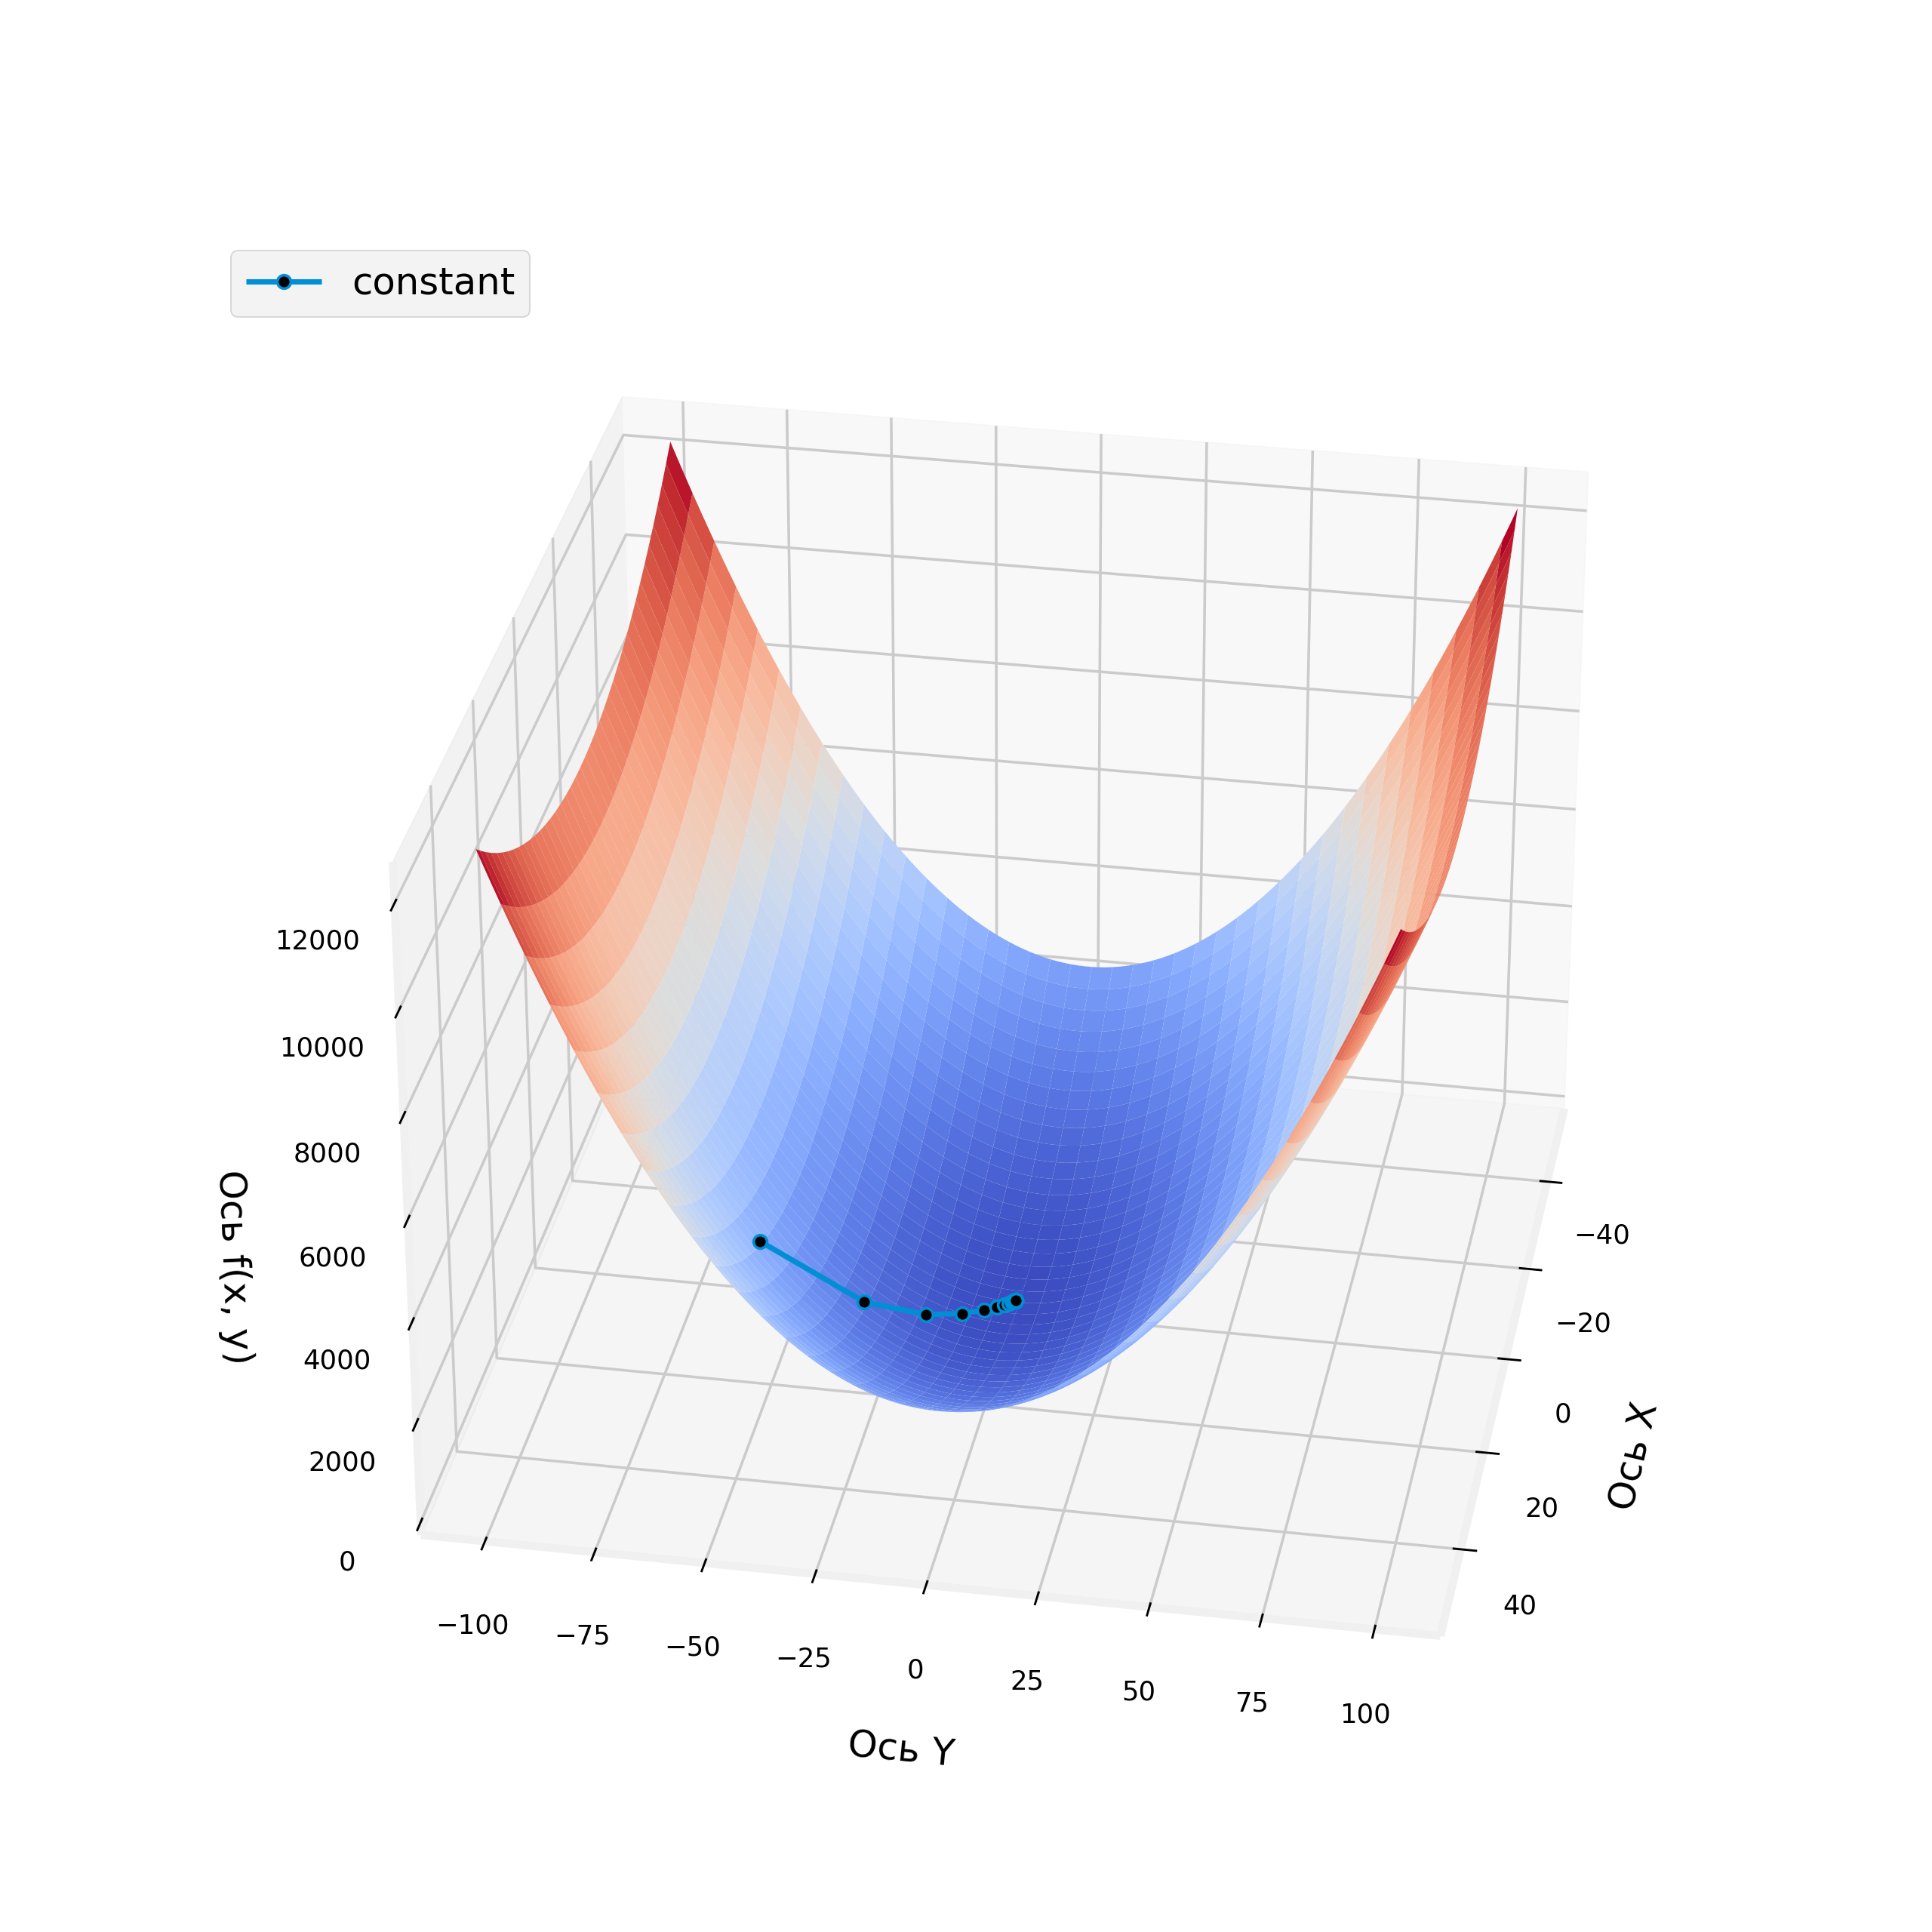
\includegraphics[scale=0.68]{Image/T1_F1.png}
		\caption*{\texttt{T1\_F1}}
	\end{figure}
	В качестве начальной точки, то есть $\text{INIT}$, установим точку $\langle 25, ~ -50 \rangle$ и понаблюдаем. Замечаем очевидный факт: оно ни к чему не стремится и явно этого не хочет, ведь мы задали ему длинный шаг и уж так получилось, что в связи с градиентом функции в $2x + 2y$, мы получаем следующие первые шаги нашего алгоритма:
	\begin{table}[H]
		\centering
		\begin{tabular}{|c|c|c|}
			\centering
			\bfseries X & \bfseries Y & \bfseries F(X, Y)
			\csvreader[head to column names]{Data/T1_F1.csv}{}
			{\\\hline\X & \Y & \F}
		\end{tabular}
		\caption*{\texttt{T1\_F1}}
	\end{table}
	Подытожим результат. При выборе функции и, особенно важно, для него шага всегда следует посмотреть на хотя бы первые значения прохода алгоритма. Вполне вероятно, Вам может понадобится другой $learning~rate$ или же, на крайний случай, другая функция.
	\subsection*{Пример 2: <<Длин-н-н-н-ый путь вниз>>}
	А теперь для эксперимента возьмем не сходящуюся функцию и посмотрим на вывод в виде шагов алгоритма. Пусть $f(x, y) = -0.84233647 \cdot x^{2} + -0.28077882 \cdot y^{2}$, здесь мы зададим ему шаг в $0.1$ и начальные координаты $\langle 0.00000014, ~ 0.1 \rangle$~-- максимум функции. Посмотрим на полученный результат:
	\begin{figure}[H]
		\centering
		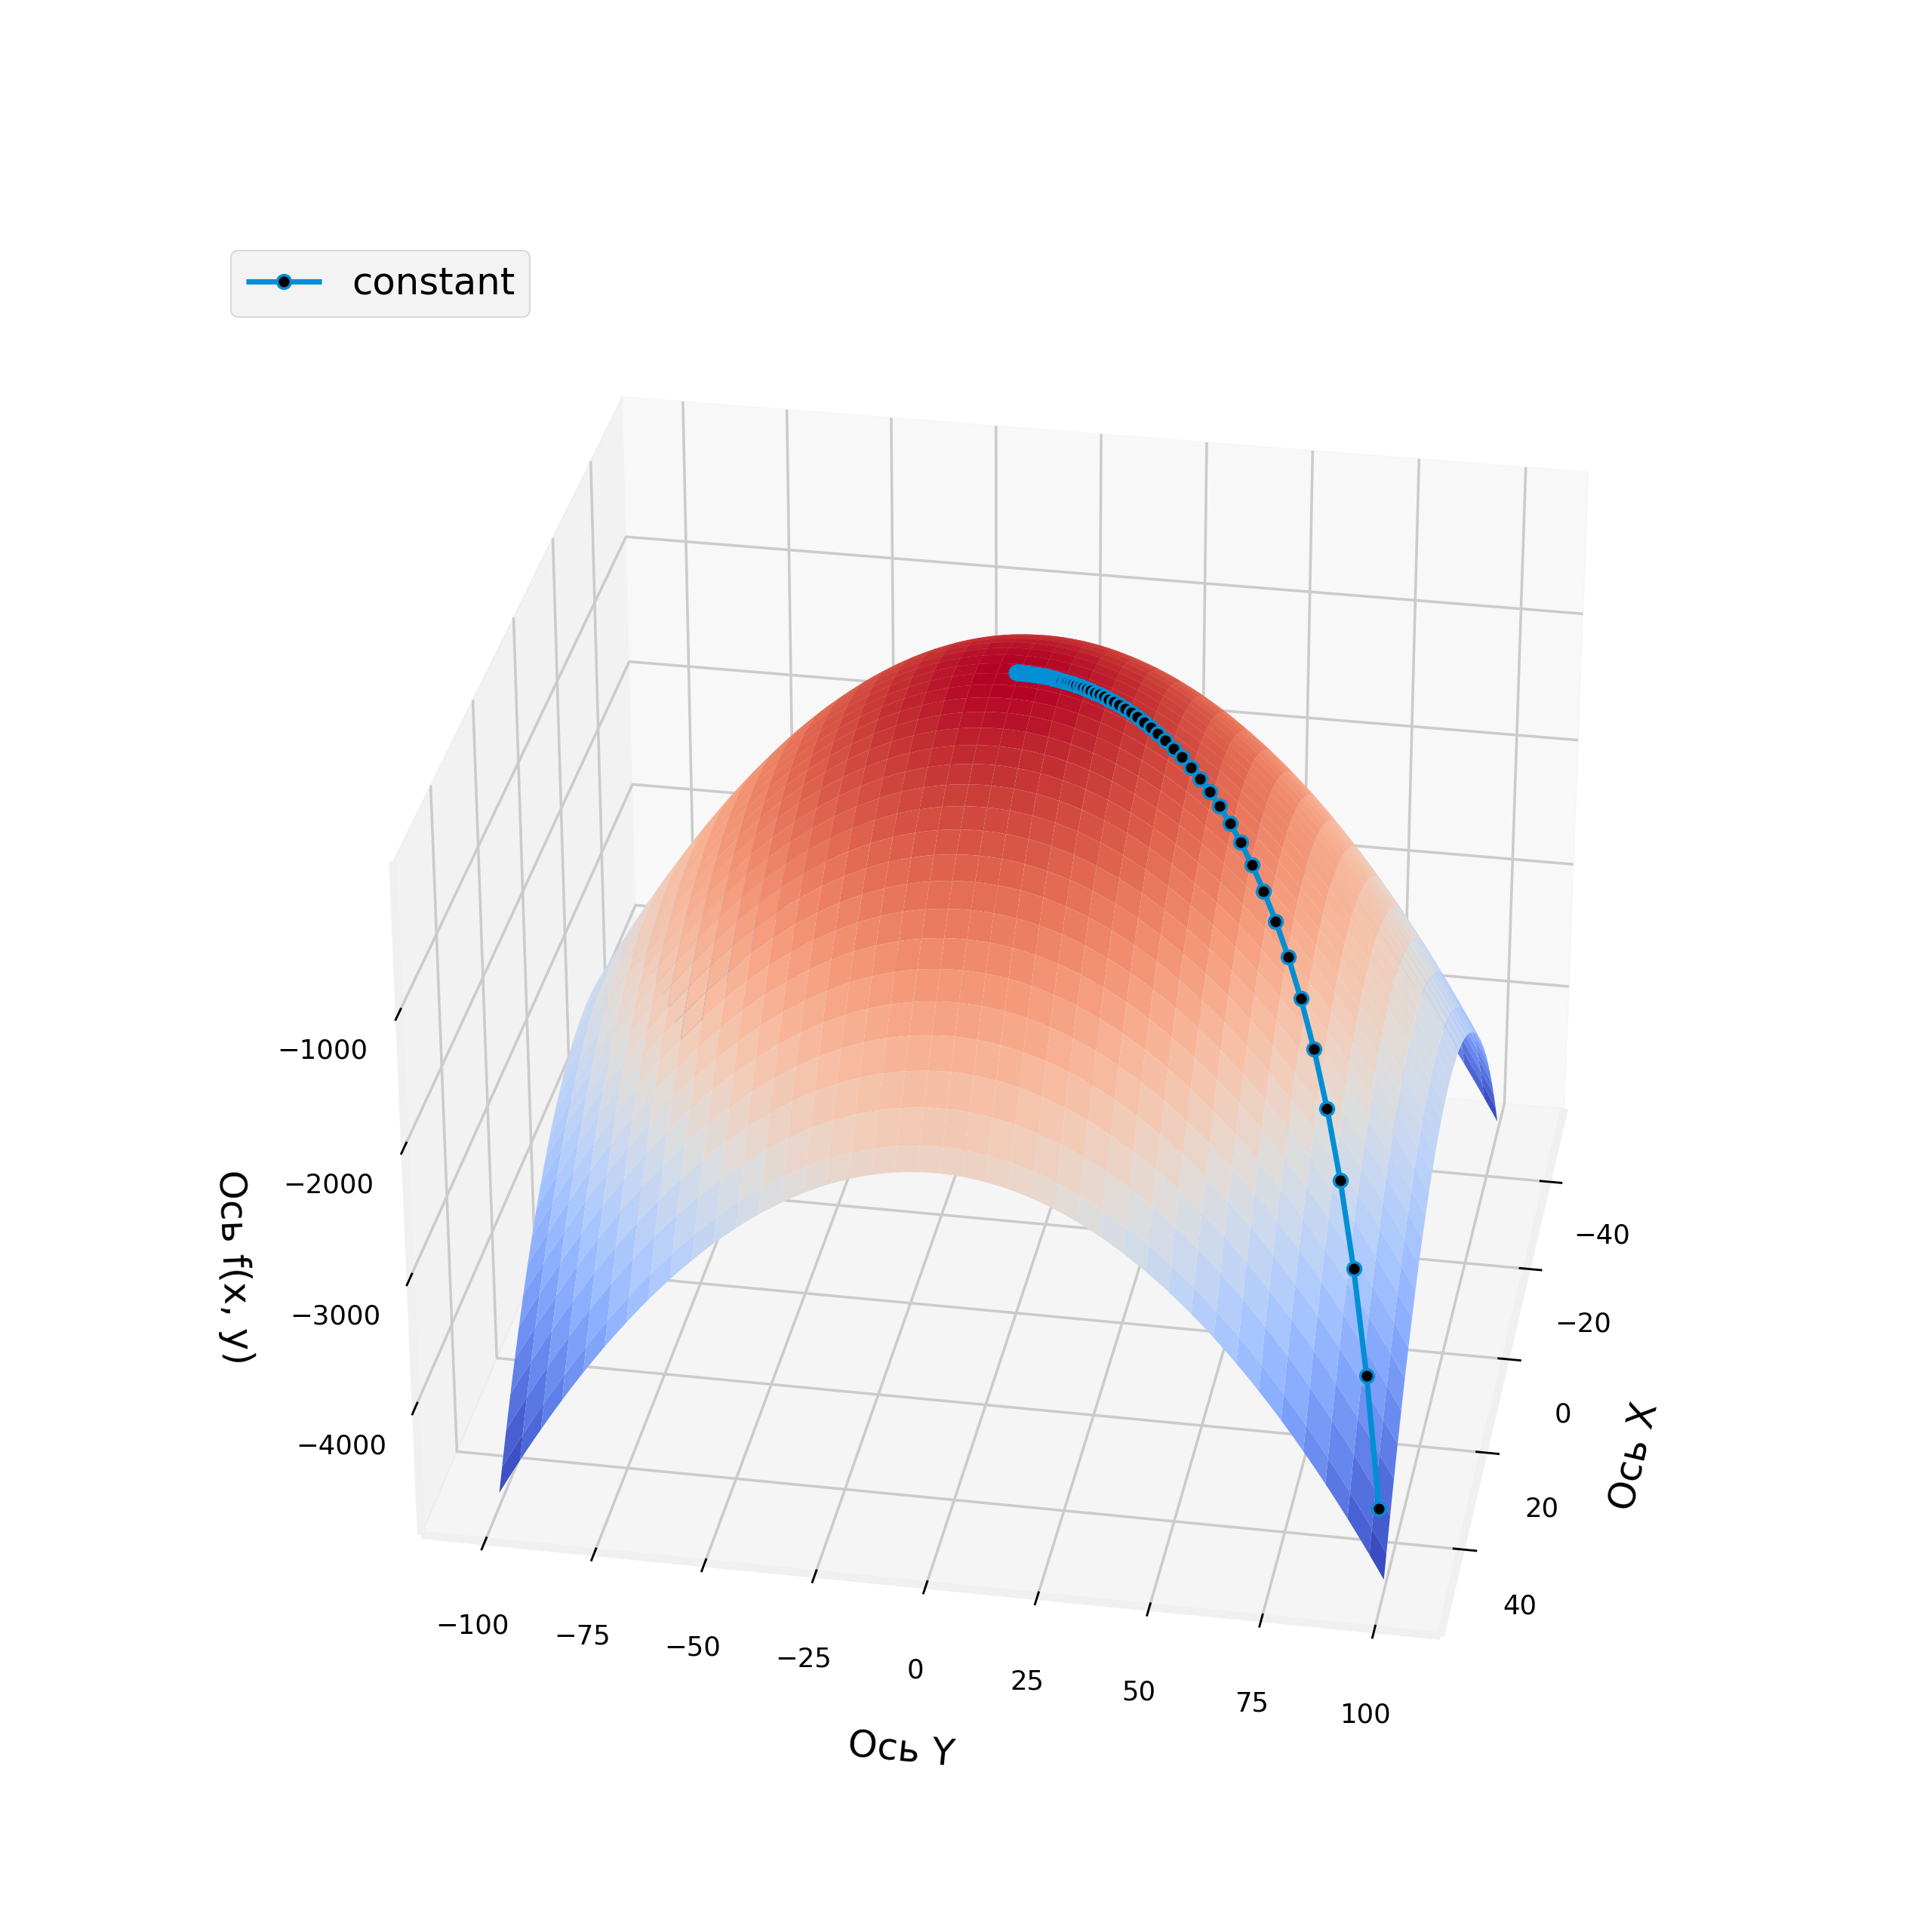
\includegraphics[scale=0.68]{Image/T1_F2.png}
		\caption*{\texttt{T1\_F2}}
	\end{figure}
	Понятное дело, как и было сказано, градиентный путь идет вниз бесконечно к лепесточкам, достигая до предельной точки заданной плоскости. И посмотрим на наши первые и последние чудесные бесконечные шаги:
	\begin{table}[H]
		\centering
		\begin{tabular}{|c|c|c|}
			\textbf{X} & \textbf{Y} & \textbf{F(X, Y)} \\ \hline
			1.4e-07&0.1&-0.00280779 \\ \hline
			1.63679e-07&0.105616&-0.00313199 \\ \hline
			1.91304e-07&0.111546&-0.00349362 \\ \hline
			2.23614e-07&0.11781&-0.00389702 \\ \hline
			2.61344e-07&0.124426&-0.00434698 \\ \hline
			3.05493e-07&0.131413&-0.00484891 \\ \hline
			3.57014e-07&0.138793&-0.00540879 \\ \hline
			4.17296e-07&0.146587&-0.00603331 \\ \hline
			4.87725e-07&0.154819&-0.00672995 \\ \hline
			5.69951e-07&0.163513&-0.00750703 \\ \hline
			6.66055e-07&0.172695&-0.00837382 \\ \hline
			7.78292e-07&0.182393&-0.00934071 \\ \hline
			9.0961e-07&0.192635&-0.0104192 \\ \hline
			1.06296e-06&0.203453&-0.0116223 \\ \hline
			1.24216e-06&0.214878&-0.0129643 \\ \hline
			1.45136e-06&0.226944&-0.0144612 \\ \hline
			1.69596e-06&0.239689&-0.0161309 \\ \hline
			1.9815e-06&0.253149&-0.0179935 \\ \hline
			...& ...& ... \\ \hline
			15.6295&66.6236&-1452.06 \\ \hline
			18.2625&70.3649&-1671.13 \\ \hline
			21.3392&74.3163&-1934.28 \\ \hline
			24.9341&78.4896&-2253.46 \\ \hline
			29.1347&82.8972&-2644.5 \\ \hline
			34.043&87.5524&-3128.49 \\ \hline
			39.778&92.469&-3733.63 \\ \hline
			46.4793&97.6617&-4497.73
		\end{tabular}
	\end{table}
	Совершенно очевидно по первым и последним шагам алгоритма, что наш спуск, как и верно направлению антиградиента действительно быстрее и быстрее по вектору наибыстрейшему направлению, что, в каком-то плане, также доказывает правильность нашего алгоритма в плане работоспособности.
	\subsection*{Пример 3, или анонс к \textit{задаче 3}}
	Наконец, последний, функцией, которая, возможно, является некоторым анонсом к задаче 3, где мы будем рассматривать странные функции, вроде этой. Итак, пусть $f(x, y) = (x^{2} - y^{2} - 9) \cdot \cos(2 \cdot x + 1 - e^{y})$. Зададим в качестве множества $\text{INIT} = \{-0.1, ~ 0.4\}$ и $learning~rate = 0.07$. Тогда, наша функция представляет две видимые нам горы, которые выглядят примерно вот так:
	\begin{figure}[H]
		\centering
		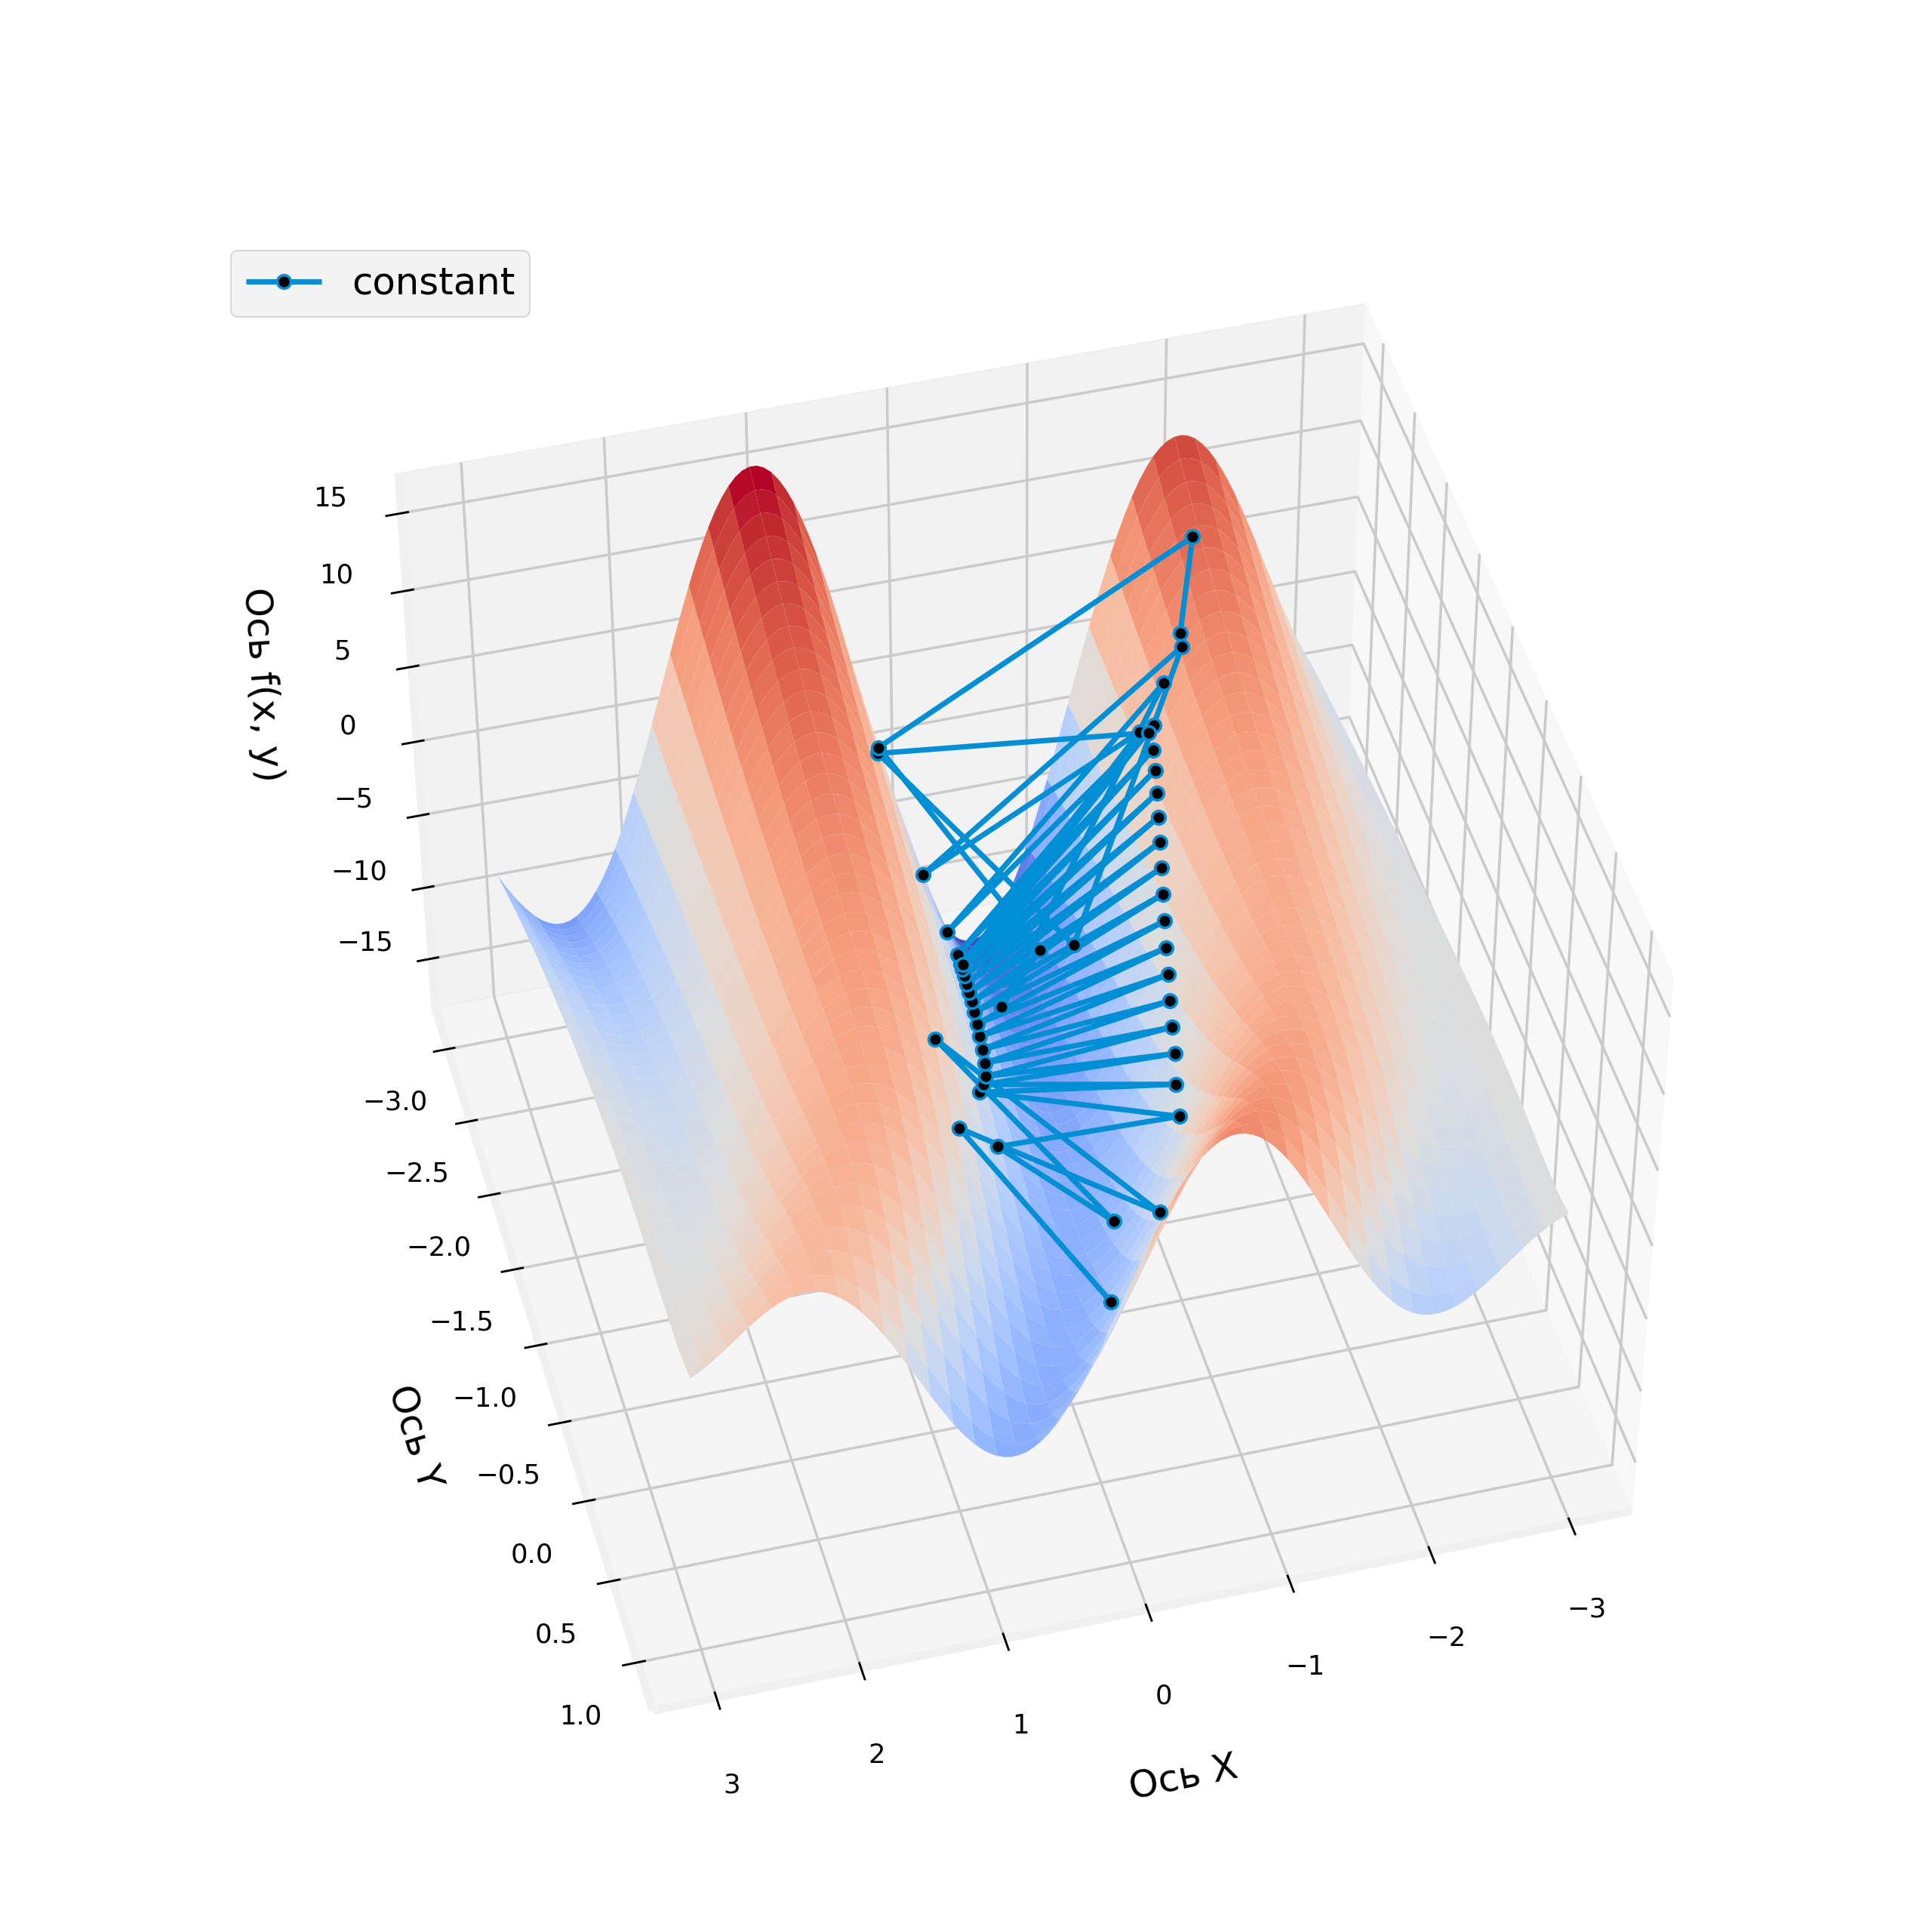
\includegraphics[scale=0.68]{Image/T1_F3.png}
		\caption*{\texttt{T1\_F3}}
	\end{figure}
	Заметим, что ситуация почти аналогична первому примеру, где алгоритм скакал меж двумя огнями, пытаясь найти минимум с слишком большим шагом. При этом, если ранее функция была симметрична относительно значений $f(x, y)$ по оси X, то здесь такого, очевидно не наблюдается, из-за чего подобное недоразумение вообще возникает. Тут даже без каких-либо данных о шагах алгоритма в виде промежуточной таблицы видно, что что-то не так или с функцией, или с методом\ldots

	В качестве промежуточного итога к именно пункту следует пояснить, что, она самом деле, по мнению автора и анализа его столь прекрасного пункта, градиентный спуск с постоянным шагом довольно-таки быстро деградирует по своей полезности, когда дело доходить либо до плохосходящихся функций (у которых все еще есть минимум, но их много на одной прямой плоскости, например) или же при похождению алгоритма найдется несколько локальных минимумов (например, это какие-то горы). В следующем задании мы узнаем, почему это так.
	\newpage
	\section*{Задача 2}
	\subsection*{Постановка задачи}
	Реализуйте метод одномерного поиска (метод дихотомии, метод Фибоначчи, метод золотого сечения) и градиентный спуск на его основе.
	\subsection*{Решение}
	Представим себе задачу: мы хотим на непрерывной функции, которая обязательно сходится к некоторому минимуму $M$, найти на некотором интервале её корень. Решая эту задачу простым способом, мы бы могли уйти в долгий, бесконечный или даже бесполезный процесс нахождения приближенного корня заданной функции $f(x)$, ведь на момент поиска мы не знаем: с какой точностью брать значение (то есть, шаг нашего поиска), в какой окрестности лежит корень на интервале (то есть, к чему нам следует сходится, чтобы успешно найти то, что мы ищем).

	Простое решение мы могли бы с легкостью заменить на тот же градиентный спуск с постоянным шагом. Однако, даже с ним мы иногда можем проиграть не только по точности приближенного минимума (если мы ищем минимум за определенное $k$ число шагов), но и вовсе уйти в бесконечный цикл (если мы ищем минимум, пока не будет выполнен критерий $|x_{i} - x_{i - 1}| \leqslant \varepsilon$, где $x_{i} = \{x^0_{i}, ~ x^1_{i}, ~ \ldots, ~ x^{n - 1}_i\}$~-- некоторая координата в $n$-мерном пространстве). По жизни чаще всего случается и другая не менее важная задача: мы хотим найти минимум как можно быстрее и скорее, причем, с точностью до предельно малого $\varepsilon$, в отличие от честного ожидания градиентного спуска.

	Для решения такой столь непосильной задачи мы воспользуемся \textit{методом дихотомии}, или же, как его еще называют, \textit{методом деления отрезка на две части}.

	Но для начала мы посмотрим на работу в одномерном пространстве. В общем случае, этот метод описывается так~-- посмотрим на текущий (может быть начальный, может быть измененный на некотором шаге) интервал $[l, r]$, выберем середину данного отрезка $x$ и сравним со знаком функции в одном из концов: при совпадении, мы перемещаем один конец интервала на точку $x$, в ином случае~-- другой. Отличие начинаются там, где мы решаем подзадачи вида поиска \textit{экстремума функции многих переменных}:
	\[
		\eth = \operatorname*{argmin}_{\eth \in [l, r]}{f(x)}
	\]
	В этом случае на последнем шаге мы смотрим не на знак, а на значение функции $f(x \pm \varepsilon)$ и также здесь смотрим на то, что мы хотим найти: если минимум, то перебрасываем правый конец в рассмотренную точку $x$, в ином случае~-- левый.

	Обозначим за $\varepsilon$~-- как некоторая окрестность минимума, $l, r \in \mathbb{R}$, задана $f(x) : \mathbb{R} \to \mathbb{R}$. Тогда, в качестве промежуточного итога предоставим псевдо-алгоритм для решения этой задачи:
	\begin{lstlisting}
	function $f(x)$:
		/*$implementation~defined$*/

	function $dichotomy2d(l, ~ r, ~ \varepsilon)$:
		$x \gets l$
		$\forall~\infty$:
			$m \gets \dfrac{x + r}{2}$
			$f_{1} \gets f(m + \varepsilon)$
			$f_{2} \gets f(m - \varepsilon)$

			if $|f_{1} - f_{2}| < \varepsilon$ then
				$r \gets m$
			else
				$x \gets m$
	\end{lstlisting}
	Теперь рассмотрим иной, более общий случай, $n$-мерный. Порассуждаем, в чем была проблема градиентного спуска: в описанном выше алгоритме цикл хода по направлению антиградиента (то есть, наискорейшего спуска) ничего не мог сделать в тех случаях, когда до приближенного минимума остается сделать не один гигантский шаг в $learning~rate$ величину, а поменьше, в точности до некоторого малого $\varepsilon$.

	Для исправления столь шальной ситуации, когда алгоритм, который работает не на количество шагов, а~-- на критерий, то есть когда время ожидания отклика программы потребует века, мы будем либо уменьшать шаг в только тех случаях, когда на заданном шаге есть пренеприятный шпион в виде локального минимум на это отрезке, либо не изменять, то есть когда локального минимума нет, а значит нам незачем как-то останавливаться на достигнутом и куда-то сворачивать. Для этого введем специальную функцию $g : [0, 1]$, которая будет возвращать $scale$ нашего шага, причем, так как мы ищем лишь окрестность желаемой точки, то возвращаемое значение будет также учитывать поданный нам $\varepsilon$. Обозначим за $x_{i} = \{x^0_{i}, ~ x^1_{i}, ~ \ldots, ~ x^{n - 1}_i\}$~-- координата точки в $n$-мерном пространстве, $f(x)$~-- заданная функция, $\nabla{f(x)}$~-- градиент функции. Идея~-- изначально мы посчитаем $f(x_{i - 1})$ и $\nabla{f(x_{i - 1})}$, передадим их в функцию для подсчета $scale$, а дальше что есть сил мы будем делать это много раз:
	\begin{enumerate}[(1)]
		\item Положим $m \gets \dfrac{l + r}{2}$ и $\alpha \gets m \pm \varepsilon$.
		\item В качестве $a$ и $b$ разность поданного сверху $f(x_{i - 1})$ и произведения $\nabla{f(x_{i - 1})}$ и $\alpha$.
		\item Рассмотрим два случая: в том случае, если $a < b$, то это значит, что приближенный минимум находится чуть подальше, но может находиться раньше границы шага, однако в ином же случае~-- точка находится много раньше, чем актуальная длина шага. Таким образом, в первом~-- мы смещаем левую границу, а в втором~-- правую.
	\end{enumerate}
	В качестве промежуточного итога предоставим псевдо-алгоритм для решения этой задачи:
	\begin{lstlisting}
	function $f(x)$:
		/*$implementation~defined$*/

	function $\nabla{f(x)}$:
		return $\left[f(x)\dfrac{\partial}{\partial{x^{0}}}, ~ f(x)\dfrac{\partial}{\partial{x^{1}}}, ~ \ldots, ~ f(x)\dfrac{\partial}{\partial{x^{n - 1}}}\right]$

	function $scale(p_1, ~ p_2)$:
		$l, r \gets 0, 1$
		$\forall~\infty$:
			$m \gets \dfrac{l + r}{2}$
			$\alpha \gets \lambda \cdot (m \pm \varepsilon)$
			$a, b \gets p_1 - p_2 \cdot \alpha$

			if $a < b$ then
				$l \gets m$
			else
				$r \gets m$

			if $|l - r| \leqslant \varepsilon$ then
				break

	function $gradient\_dichotomy$:
		$x_{0} \gets \text{INIT}$
		$\lambda \gets \texttt{const}$
		$\forall~i \in [1, k]$:
			$x_{i} \gets x_{i - 1} - \lambda \cdot \texttt{scale}(f(x_{i - 1}), \nabla{f(x_{i - 1})})$
	\end{lstlisting}
	\subsection*{Пример 1: <<\texttt{scipy.optimize.rosen}>>}
	Посмотрим на функцию Розенброка, которая, как мы знаем, выглядит вот так: $f(x, y) = (1 - x)^{2} + 100 \cdot (y - x^2)^2$ в трехмерном пространстве (мы, как мы помним, договорились об этом раньше). Она имеет глобальный минимум в точке $\langle 1, ~ 1 \rangle$, где $f(x, y) = 0$. Положим $\text{INIT} = \{0.4, ~ -0.9\}$, а шагом алгоритма установим $learning~rate = 0.005$ для градиентного спуска. Запустим же нашего зверя на добычу и посмотрим на результат.
	\begin{figure}[H]
		\centering
		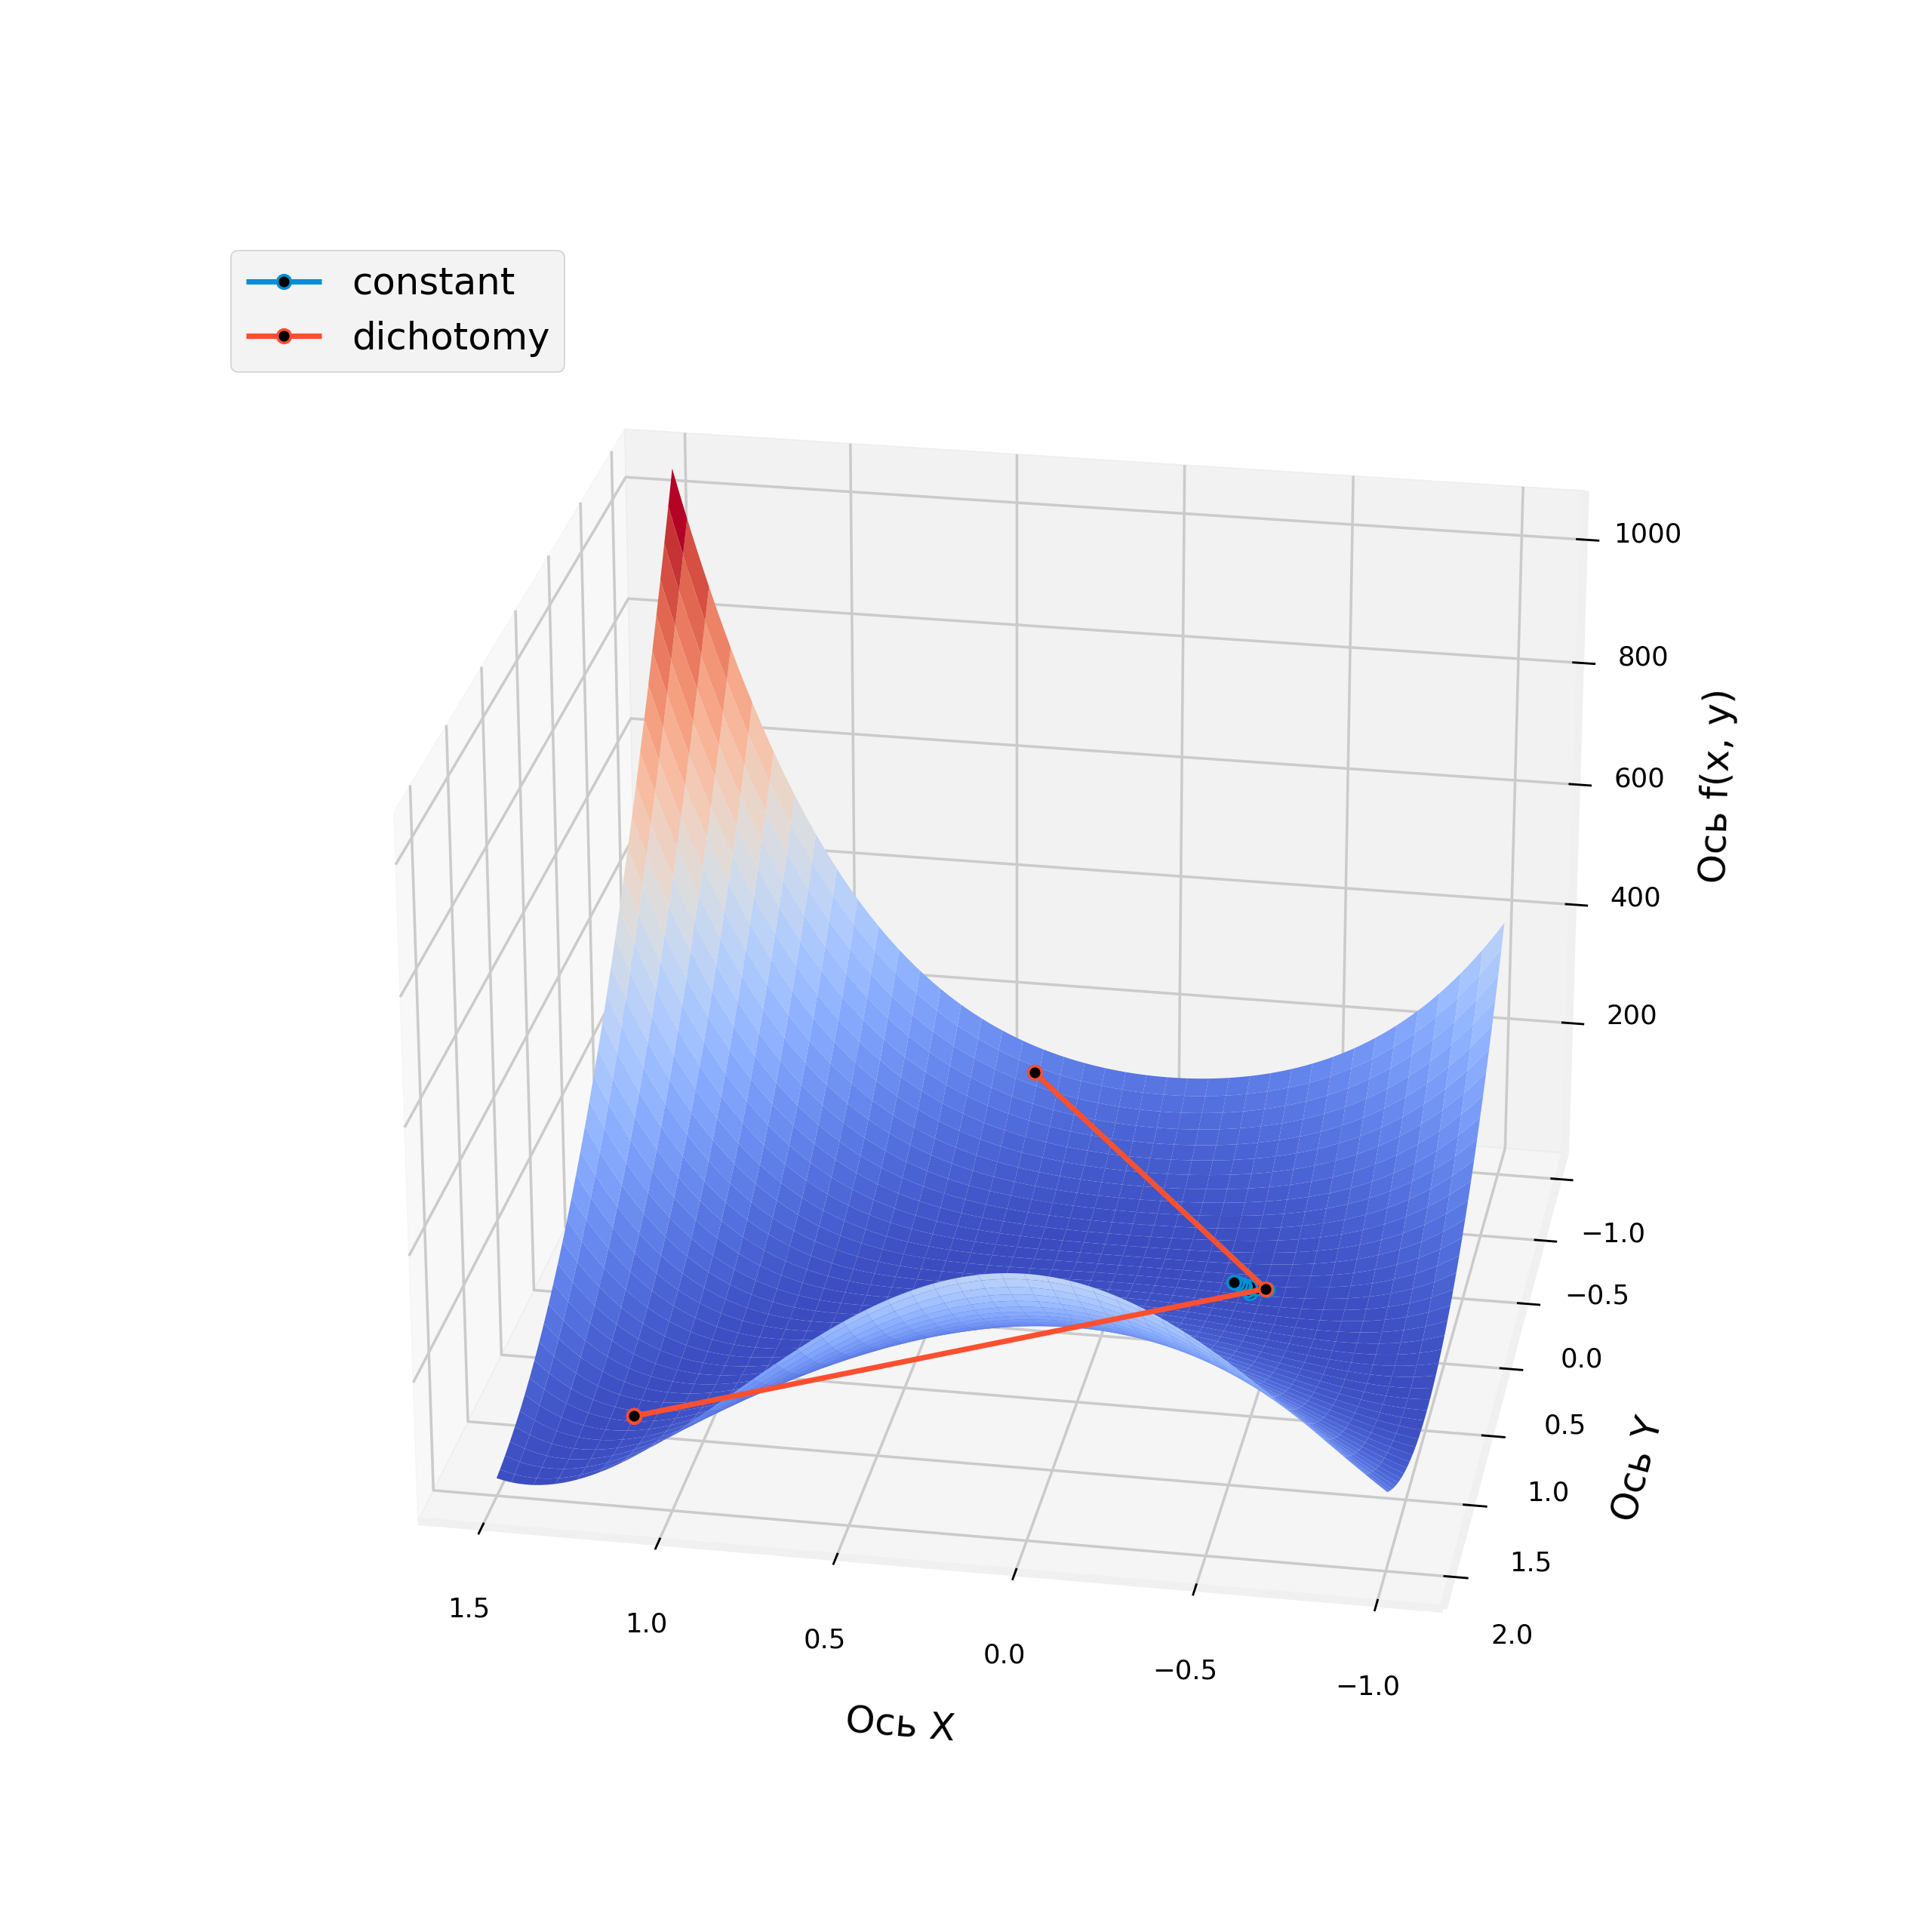
\includegraphics[scale=0.68]{Image/T2_F1.png}
		\caption*{\texttt{T2\_F1}}
	\end{figure}
	Выходные данные для обоих этих методов выглядит примерно так:
	\begin{align*}
		\texttt{gradient\_descent}~&:~\langle -0.340864, ~ 0.122798\rangle \to 1.802286 \\
		\texttt{with\_dichotomy}~&:~\langle 1.206564, ~ 1.457076\rangle \to 0.042832
	\end{align*}
	Что мы здесь видим? Внезапно, но метод дихотомии, за счет возможности изменения шага, таки добирается до почти минимума поданной функции, градиентный же спуск застревает в локальном минимуме и спокойно там спит, ему там теплее. Теперь посмотрим на вывод шагов двух методов и сравним их:
	\begin{table}[H]
		\centering
		\begin{tabular}{|c|c|c|c|c|c|}
			$X_{\texttt{grad}}$ & $Y_{\texttt{grad}}$ & $Z_{\texttt{grad}}$ & $X_{\texttt{dich}}$ & $Y_{\texttt{dich}}$ & $Z_{\texttt{dich}}$ \\ \hline
			0.4&-0.9&112.72&0.4&-0.9&112.72 \\
			-0.442&0.16&2.20442&-0.43696&0.153656&2.20383 \\
			-0.396318&0.195364&2.09636&1.20755&1.45946&0.0432416 \\
			-0.41271&0.157068&2.01333&1.20775&1.45922&0.0431904 \\
			-0.387637&0.170329&1.9658&1.2073&1.45886&0.0431392 \\
			-0.389318&0.150262&1.93037&1.2075&1.45862&0.043088 \\
			-0.374408&0.151568&1.90196&1.20706&1.45827&0.0430368 \\
			-0.369191&0.140181&1.87619&1.20725&1.45802&0.0429856 \\
			-0.358363&0.136302&1.85136&1.20681&1.45767&0.0429344 \\
			-0.350426&0.128424&1.82681&1.20701&1.45743&0.0428833 \\
			-0.340864&0.122798&1.80229&1.20656&1.45708&0.0428322
		\end{tabular}
	\end{table}
	Дихотомия, как и по красивой картинке, практически сразу же добралась до минимума и никак (на самом деле, по некоторому предельно малому значению $\varepsilon$) почти не менялась. Градиентный спуск обычный же сделал несколько бодрых правильных шагов, но затем погряз в коррупции и оказался почти на дне, никуда не уходя и не развиваясь, опять же по последним шагам.
	\subsection*{Пример 2: Функция Гольдшейна-Прайса}
	Еще одним примером станет ситуация, когда и тот, и другой метод верно приходят к одну минимуму, но при этом, из-за ограниченности шагов, метод дихотомии успел добраться до приближенного по модулю $\varepsilon$ значению, а градиентный спуск~-- нет.. Зададим функцию Гольдшейна-Прайса,
	\begin{align*}
		f(x, y) &= (1 + (x + y + 1)^2 \cdot (19 - 14 \cdot x + 3 \cdot x^2-14 \cdot y + 6 \cdot x \cdot y + 3 \cdot y^2)) \\
		&\cdot ((30 + (2 \cdot x - 3 \cdot y)^2 \cdot (18 - 32 \cdot x + 12 \cdot x^2 + 48 \cdot y - 36 \cdot x \cdot y+27 \cdot y^2))
	\end{align*}
	В качестве начальных координат мы положим $\langle -0.9, ~ 0.7\rangle$, а шаг градиентного спуска положим $0.000005$, для дихотомии~-- $0.8$. Почему именно такие значения, потому-что функция плохообсусловена и при выборе большим шагом градиентный спуск убегает за пределы даже рассматриваемой плоскости, именно поэтому выбираем такие значения. Запустим алгоритм и посмотрим на результат.
	\begin{figure}[H]
		\centering
		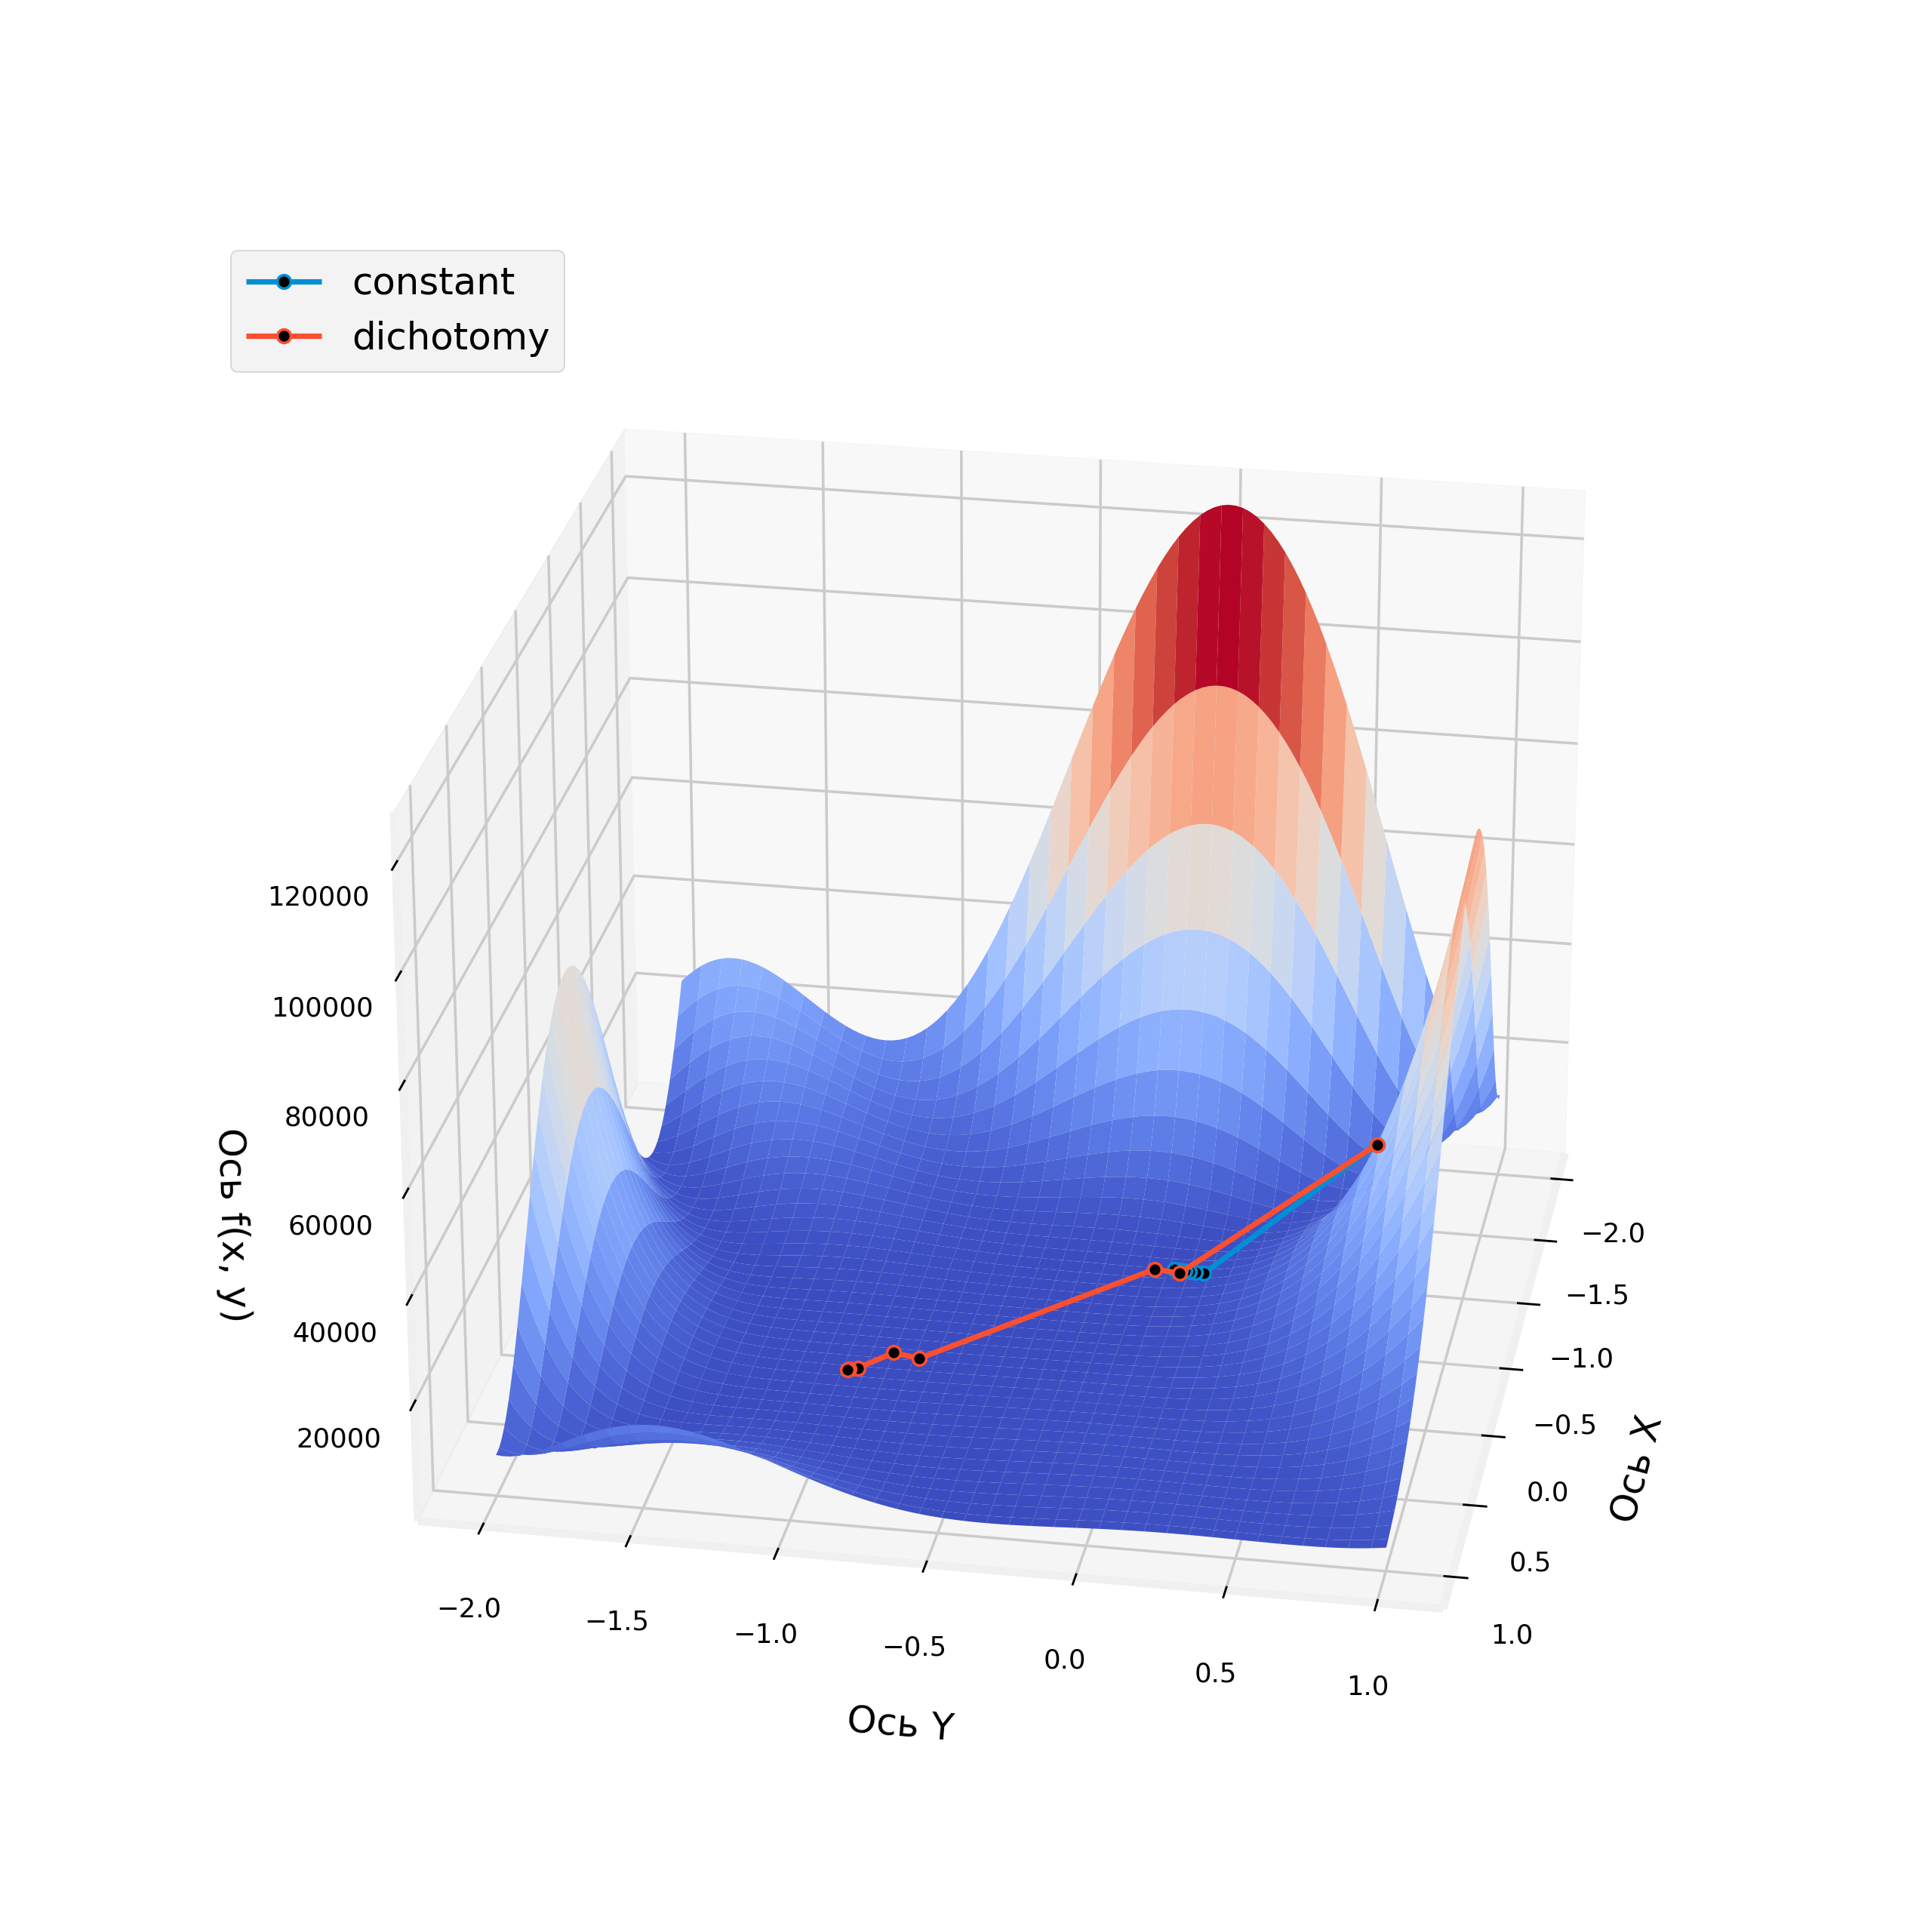
\includegraphics[scale=0.68]{Image/T2_F2.png}
		\caption*{\texttt{T2\_F2}}
	\end{figure}
	За первый шаг алгоритмов и градиентный спуск, и с методом дихотомии шагнули в одном направлении и попали в неподалеку расположенные точки. Затем оба начинают двигаться в направлении минимума. Но, как мы видим, дальше, за счет нехватки количества доступных шагов алгоритма, градиентный спуск не поспевает за дихотомией и как бы <<застревает в локальном>>, но, на самом деле, если увеличить количество шагов до какого-то большого значения, то спуск начинает двигаться медленно и верно.
	\newpage
	\section*{Задача 3}
	\subsection*{Постановка задачи}
	Проанализируйте траекторию градиентного спуска на примере квадратичных функций. Для этого придумайте две-три квадратичные функции от двух переменных, на которых работа методов будет отличаться.
	\subsection*{Решение}
	В жизни любого человека приходит момент, когда ему наверняка захочется сравнить две изученные им темы и посмотреть, кто же из них более эффективный и правильный в плане выполнения изначально заданной задачи. Методы, используемые в этом задании, уже были подробно разобраны в первом и во втором задании. Кратко напомним псевдо-код алгоритма градиентного спуска:
	\begin{lstlisting}
	function $f(x)$:
		/*$implementation~defined$*/

	function $\nabla{f(x)}$:
		return $\left[f(x)\dfrac{\partial}{\partial{x^{0}}}, ~ f(x)\dfrac{\partial}{\partial{x^{1}}}, ~ \ldots, ~ f(x)\dfrac{\partial}{\partial{x^{n - 1}}}\right]$

	function $gradient(f(x))$:
		$x_{0} \gets \text{INIT}$
		$\lambda \gets \texttt{const}$
		$\forall i \in [1, k]$:
		    $x_{i} \gets x_{i - 1} - \lambda \cdot \nabla{f(x_{i - 1})}$
	\end{lstlisting}
	И для градиентного спуска на основе метода дихотомии:
	\begin{lstlisting}
	function $f(x)$:
		/*$implementation~defined$*/

	function $\nabla{f(x)}$:
		return $\left[f(x)\dfrac{\partial}{\partial{x^{0}}}, ~ f(x)\dfrac{\partial}{\partial{x^{1}}}, ~ \ldots, ~ f(x)\dfrac{\partial}{\partial{x^{n - 1}}}\right]$

	function $scale(p_1, ~ p_2)$:
		$l, r \gets 0, 1$
		$\forall~\infty$:
			$m \gets \dfrac{l + r}{2}$
			$\alpha \gets \lambda \cdot (m \pm \varepsilon)$
			$a, b \gets p_1 - p_2 \cdot \alpha$

			if $a < b$ then
				$l \gets m$
			else
				$r \gets m$

			if $|l - r| \leqslant \varepsilon$ then
				break

	function $gradient\_dichotomy$:
		$x_{0} \gets \text{INIT}$
		$\lambda \gets \texttt{const}$
		$\forall~i \in [1, k]$:
			$x_{i} \gets x_{i - 1} - \lambda \cdot \texttt{scale}(f(x_{i - 1}), \nabla{f(x_{i - 1})})$
	\end{lstlisting}
	Как уже было сказано ранее, градиентный спуск проигрывает на неочевидных и не тривиальных функциях. Метод дихотомии же, по второму пункту, успешно справлялся с простыми случаям. Посмотрим на то, как будет справляться это метод на квадратичных функциях.
	\subsection*{Пример 1}
	В качестве первого примера мы возьмем уже знакомого нам друга~-- $f(x, y) = x^{2} + y^{2}$. Зададим вновь $learning~rate = 1$ для градиентного спуска, специально для того, чтобы шаг алгоритма был повторяющийся для демонстрации работы метода дихотомии на той же функции с тем же $learning~rate$. Также зададим начальной точкой точку $\langle 35, ~ 50 \rangle$ и максимальным количеством шагов в $60$. Запустим же алгоритмы и посмотрим на результат.
	\begin{figure}[H]
		\centering
		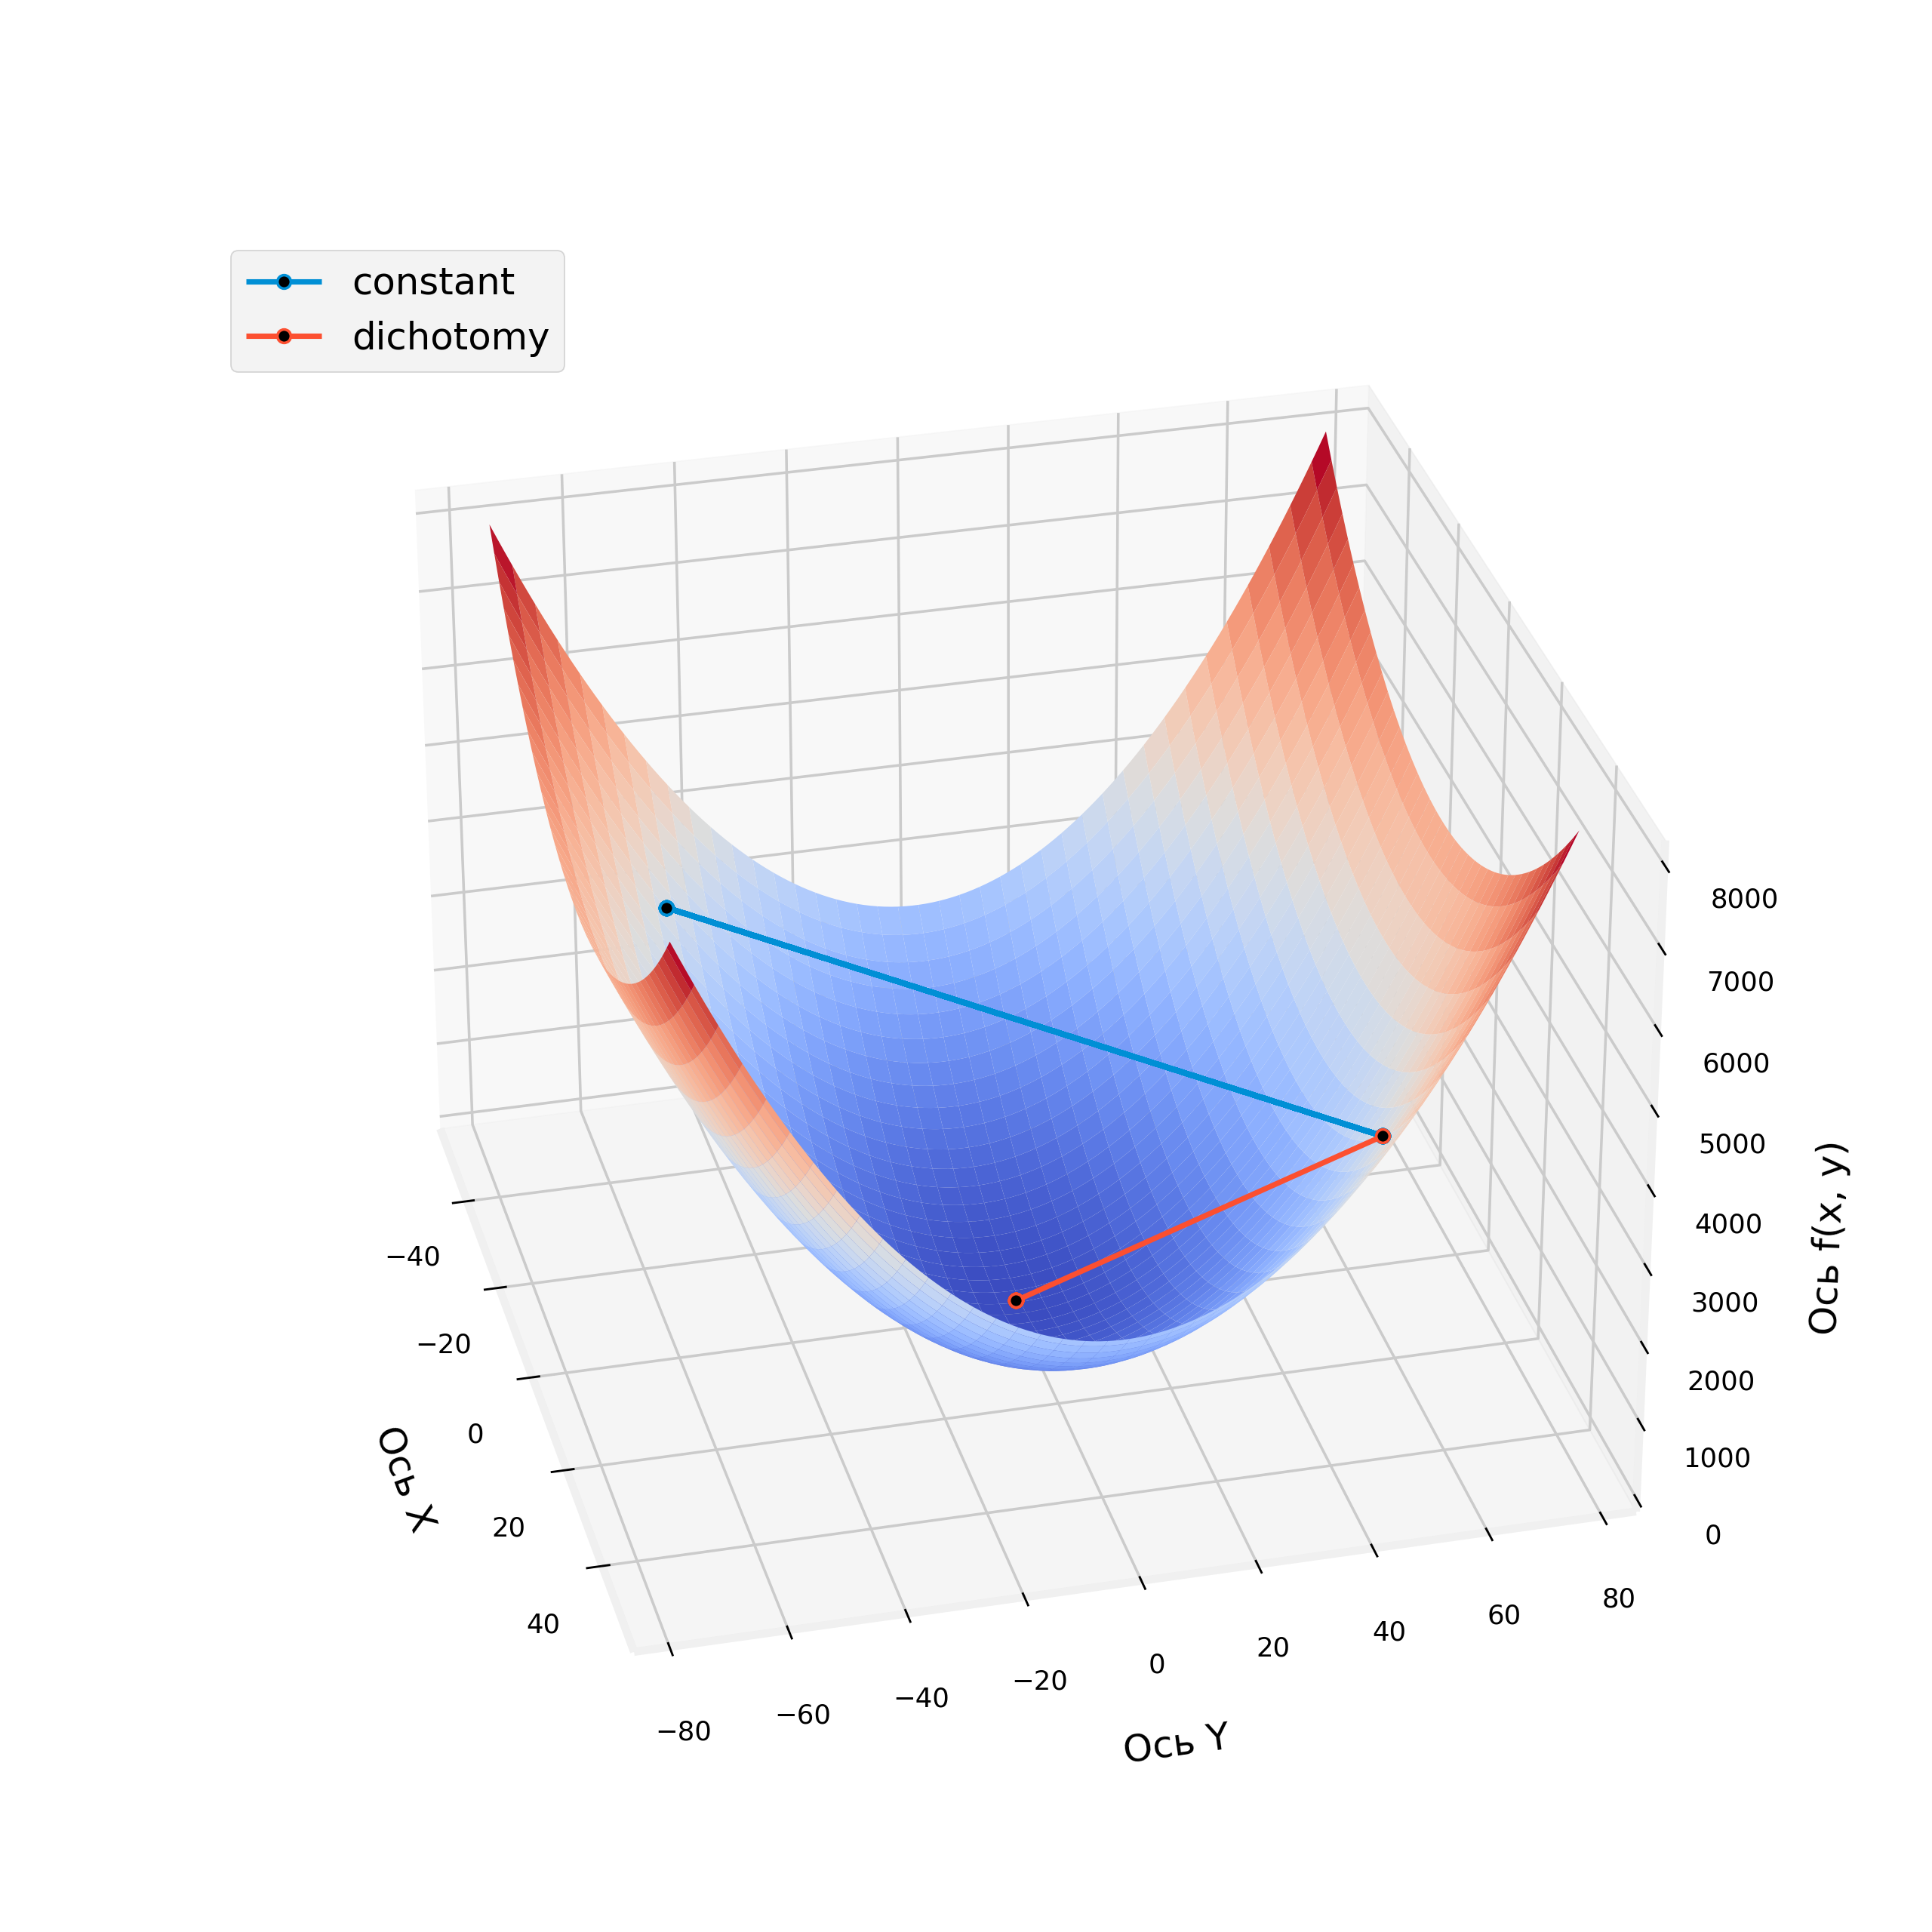
\includegraphics[scale=0.68]{Image/T3_F1.png}
		\caption*{\texttt{T3\_F1}}
	\end{figure}
	Как уже было замечено в первом задании лабораторной работы, градиентный спуск, в виду специфики симметричной функции, по проводимому алгоритму прыгает из одного места в другое. А что же с методом дихотомии? Первым шагом дихотомия с точки $\langle 35, ~ 50\rangle$ попадает в точку $\langle 4.263e-05, ~  -6.90283e-05\rangle$~-- второй шаг и последний шаг первого метода перед циклом. Далее, вторым шагом алгоритма, в отличие от обычного градиентного спуска, версия с методом дихотомии меняет размер свой шаг в зависимости от значения функции в точке и градиента в сторону уменьшения и, как показано, успешно выбирает такое значение $scale$, что следующий шаг переходит из $\langle 4.263e-05, ~  -6.90283e-05\rangle$ в $\langle -6.21967e-10, ~ -3.0251e-10\rangle$. Остальные итерации версии метода дихотомии представляют из себя коррекцию минимального значения функции.
	Далее представлена таблица первых нескольких и последних шагов алгоритма:
	\begin{table}[H]
		\centering
		\begin{tabular}{|c|c|c|c|c|c|}
			$X_{\texttt{grad}}$ & $Y_{\texttt{grad}}$ & $Z_{\texttt{grad}}$ & $X_{\texttt{dich}}$ & $Y_{\texttt{dich}}$ & $Z_{\texttt{dich}}$ \\ \hline
			35&50&3725&35&50&3725 \\
			-34.9997&-49.9999&3724.97&4.263e-05&-6.90283e-05&6.58221e-09 \\
			34.9995&49.9991&3724.88&-6.21967e-10&-3.0251e-10&4.78355e-19 \\
			-34.9997&-49.9989&3724.87&-5.85483e-10&-3.61586e-10&4.73534e-19 \\
			...&...&...&...&...&... \\
			34.9995&49.9991&3724.88&-5.85478e-10&-3.61593e-10&4.73534e-19 \\
			-34.9997&-49.9989&3724.87&-5.85478e-10&-3.61593e-10&4.73534e-19 \\
			34.9995&49.9991&3724.88&-5.85478e-10&-3.61593e-10&4.73534e-19	
		\end{tabular}
	\end{table}
	\subsection*{Пример 2}
	Посмотрим теперь на такую немного странную в плане коэффициентов функцию:
	\[
		f(x, y) = 0.7464451039232642 \cdot x^{2} + 0.637923954128351 \cdot x \cdot y + 0.5415655721418664 \cdot y^{2}
	\]
	В отличие от предыдущей, здесь и градиентный спуск, и метод дихотомии сходятся к одной точке и не вызывают никаких дополнительных вопросов по работоспособности методов в целом. Для нее мы зададим начальные точки $\langle 50, ~ -75\rangle$ и $learning~rate = 0.2$ для обычного спуска. Посмотрим на результат работы:
	\begin{figure}[H]
		\centering
		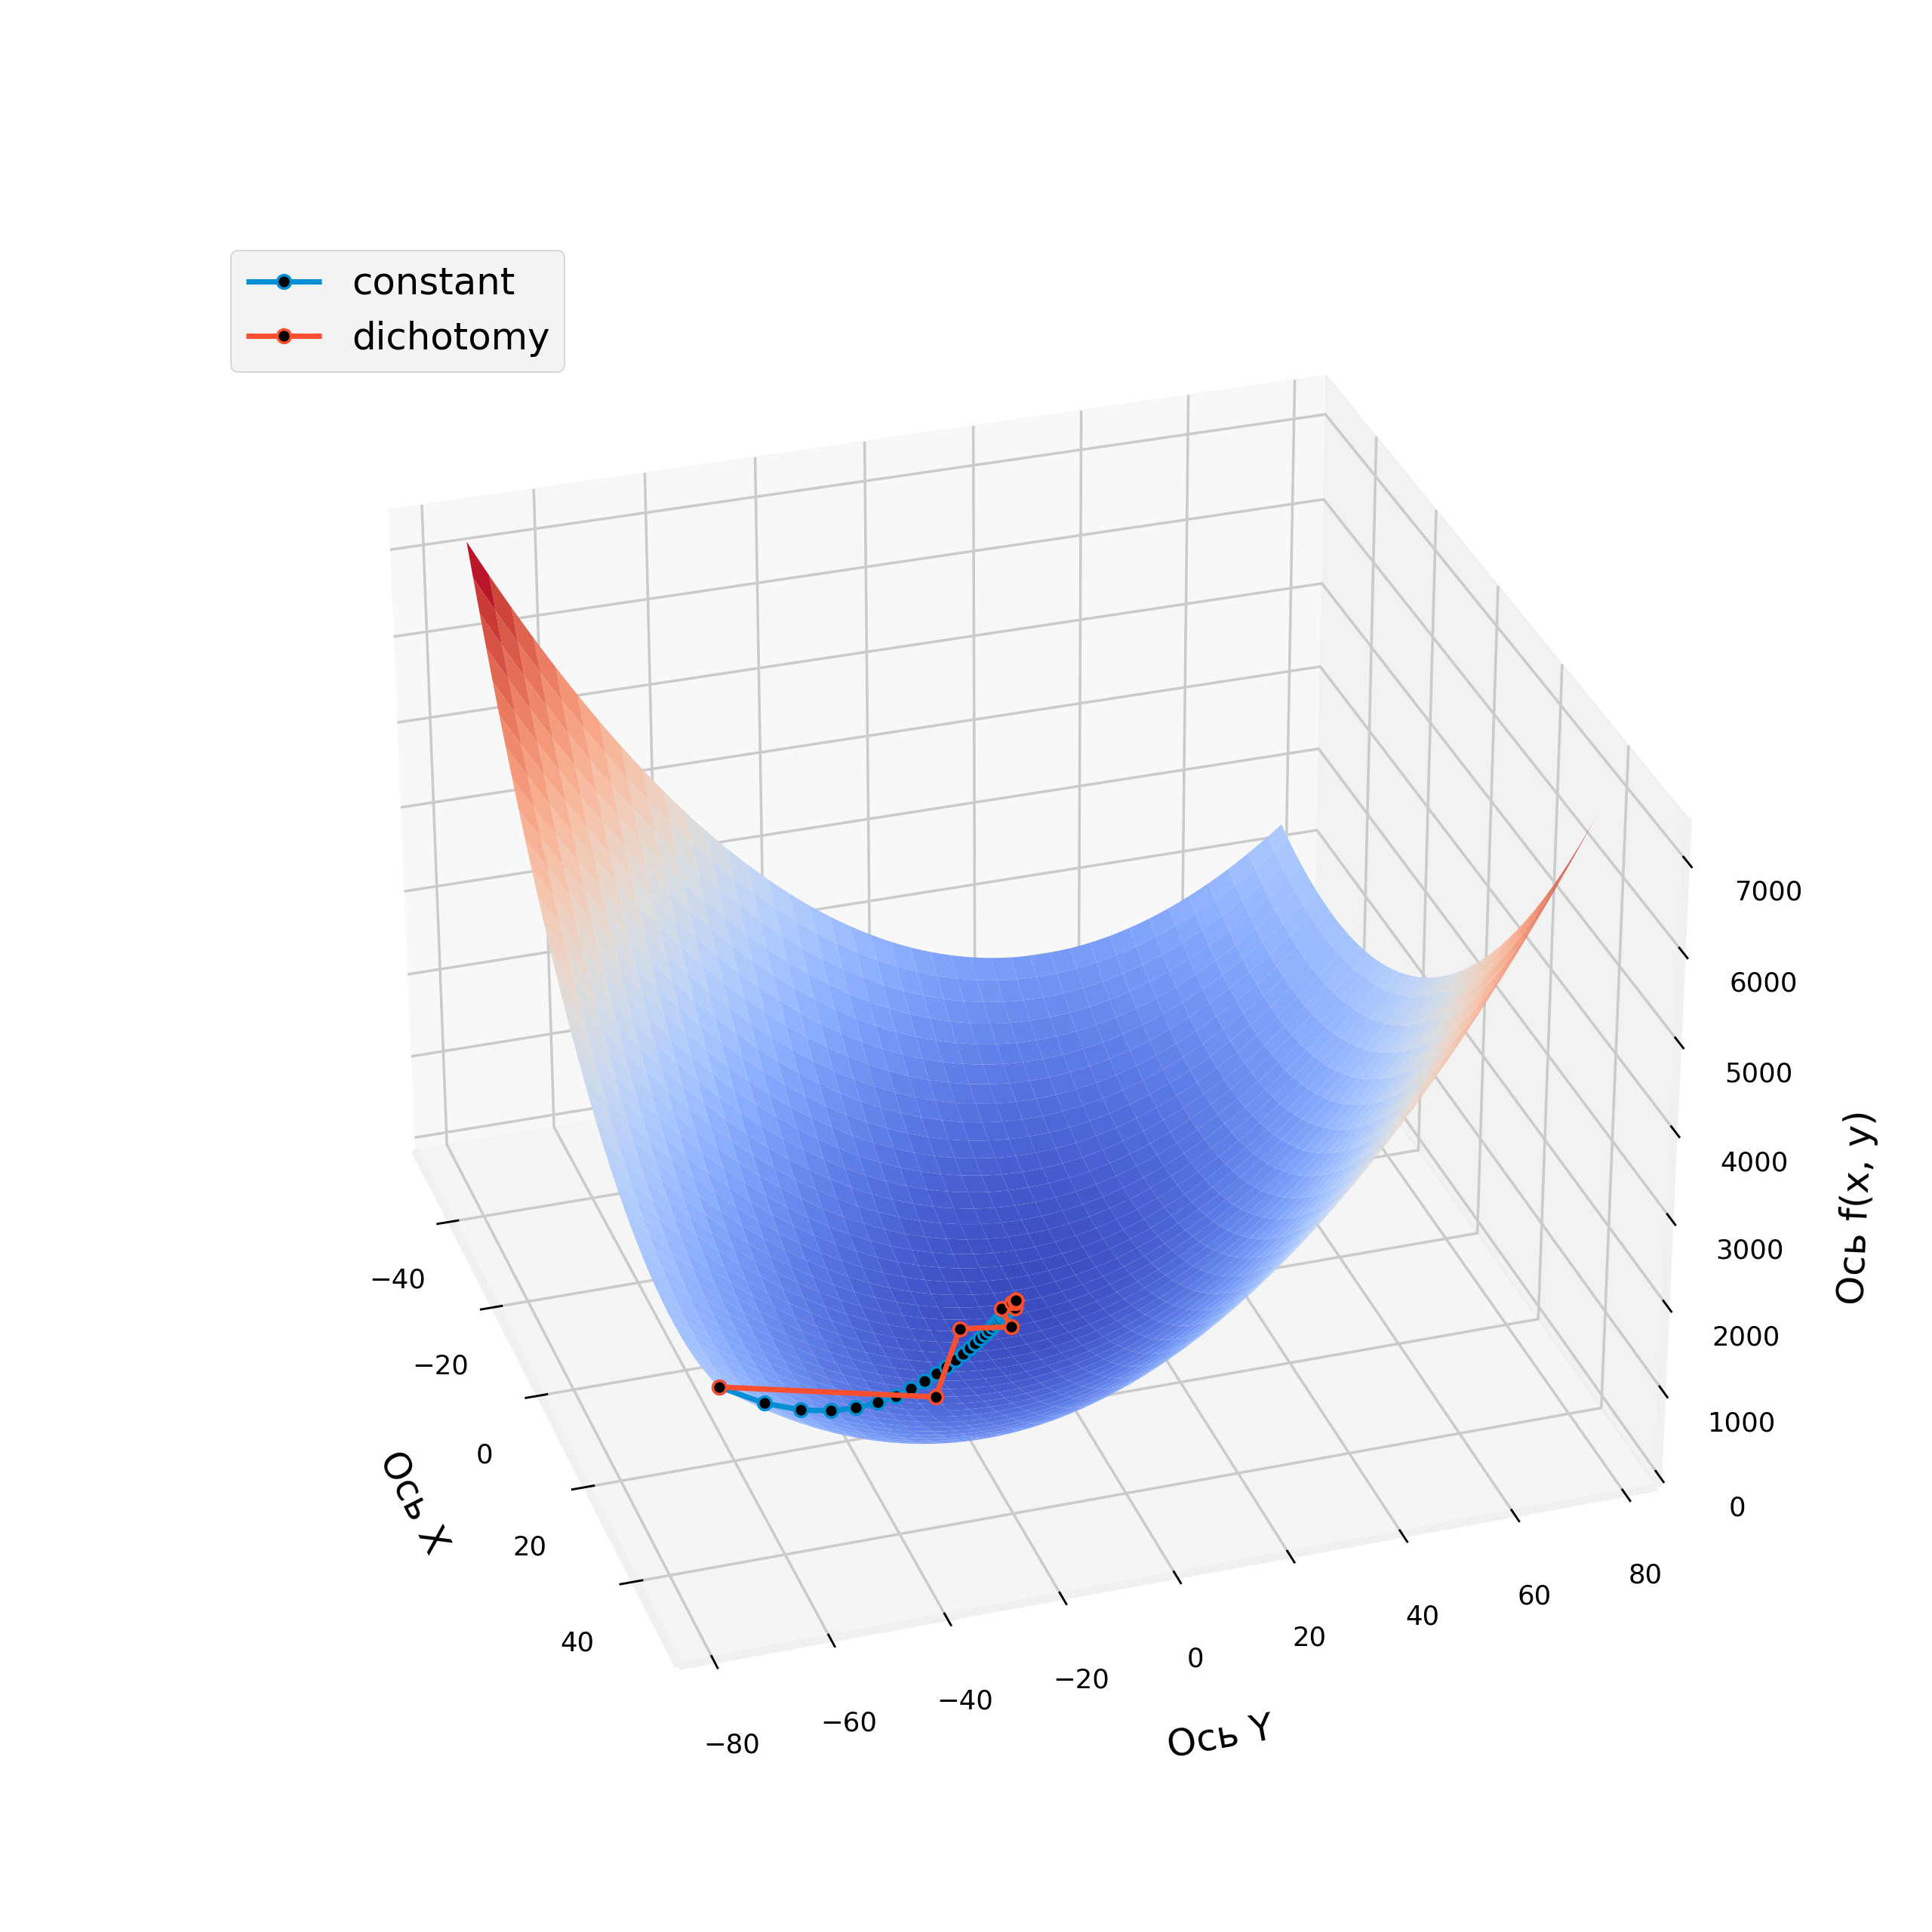
\includegraphics[scale=0.68]{Image/T3_F2.png}
		\caption*{\texttt{T3\_F2}}
	\end{figure}
	Оба метода успешно сходятся к одному и тому же минимуму, но при этом есть отличие уже в скорости: если обычный градиентный спуск добирается выданными маленькими шагами, в отличие от метода дихотомии, который быстро-быстро большими шагами доходит до некоторого точки $T$, а затем, понижая скорость, уменьшается $scale$ шага до с точности предельного малого $\varepsilon$. Последние точки, полученные при спуске, являются коррекционными при поиске минимума. В этом нам помогает убедиться таблица шагов алгоритма:
	\begin{table}[H]
		\centering
		\begin{tabular}{|c|c|c|c|c|c|}
			$X_{\texttt{grad}}$ & $Y_{\texttt{grad}}$ & $Z_{\texttt{grad}}$ & $X_{\texttt{dich}}$ & $Y_{\texttt{dich}}$ & $Z_{\texttt{dich}}$ \\ \hline
			50 & -75 & 2520.2 & 50 & -75 & 2520.2 \\
			44.64 & -65.1323 & 1930.13 & 23.1999 & -25.661 & 378.605 \\
			39.6212 & -56.7183 & 1480.43 & 4.93507 & -12.6665 & 65.1919 \\
			35.0275 & -49.4868 & 1136.32 & 5.54393 & -3.63598 & 17.2428 \\
			30.8828 & -43.2357 & 872.501 & 1.30529 & -3.3502 & 4.56059 \\
			27.178 & -37.8099 & 670.045 & 1.46633 & -0.96169 & 1.20624 \\
			... & ... & ... & ... & ... & ... \\
			0.000146876 & -0.000201437 & 1.92039e-08 & -2.94978e-10 & -3.43334e-10 & 1.93394e-19 \\
			0.000128722 & -0.00017654 & 1.47501e-08 & -2.94978e-10 & -3.43334e-10 & 1.93394e-19 \\
			0.000112812 & -0.00015472 & 1.13293e-08 & -2.94978e-10 & -3.43334e-10 & 1.93395e-19 \\
			9.88685e-05 & -0.000135596 & 8.70178e-09 & -2.94978e-10 & -3.43334e-10 & 1.93395e-19
		\end{tabular}
	\end{table}
	Приведем некоторый итог к этим двум примерам. Мы увидели, что на квадратичных функциях градиентный спуск и тот же в основе метода дихотомии работают по разному не только в плане скорости получений приближенных результатов, но и выводимых значений в качестве шагов алгоритмов: мы убедились, что при неправильных $learning~rate$ и начальных данных, метод дихотомии \textit{наверняка} сможет найти искомый приближенный минимум.
	\newpage
	\section*{Задача 4}
	\subsection*{Постановка задачи}
	Для каждой функции:
	\begin{enumerate}[(a)]
		\item исследуйте сходимость градиентного спуска с постоянным шагом, сравните полученные результаты для выбранных функций;
		\item сравните эффективность градиентного спуска с использованием одномерного поиска с точки зрения количества вычислений минимизируемой функции и ее градиентов;
		\item исследуйте работу методов в зависимости от выбора начальной точки;
		\item исследуйте влияние нормализации (scaling) на сходимость на примере масштабирования осей плохо обусловленной функции;
		\item в каждом случае нарисуйте графики с линиями уровня и траекториями методов;
	\end{enumerate}
	\subsection*{Решение пункта (a)}
	\subsubsection*{Пример 1}
	Рассмотрим функцию $f(x, y) = x^{2} + y^{2}$~-- самую простую и сходящуюся функцию из третьего задания. Для исследования сходимости с постоянным шагом мы посмотрим на количество шагов от данного конкретного постоянного шага. Здесь и в следующем примере диапазон шагов зададим $[0, 1]$ с меняющимся шагом в $10^{-3}$. В качестве $\text{INIT}$ установим значение $\langle 35, ~ 50 \rangle$. В качестве критерия остановки и здесь, и в следующем шаге положим два критерия:
	\begin{enumerate}[(1)]
		\item предельное число шагов;
		\item проверка на окрестность заранее известного минимума.
	\end{enumerate}
	Запустим алгоритм и посмотрим на график.
	\begin{figure}[H]
		\centering
		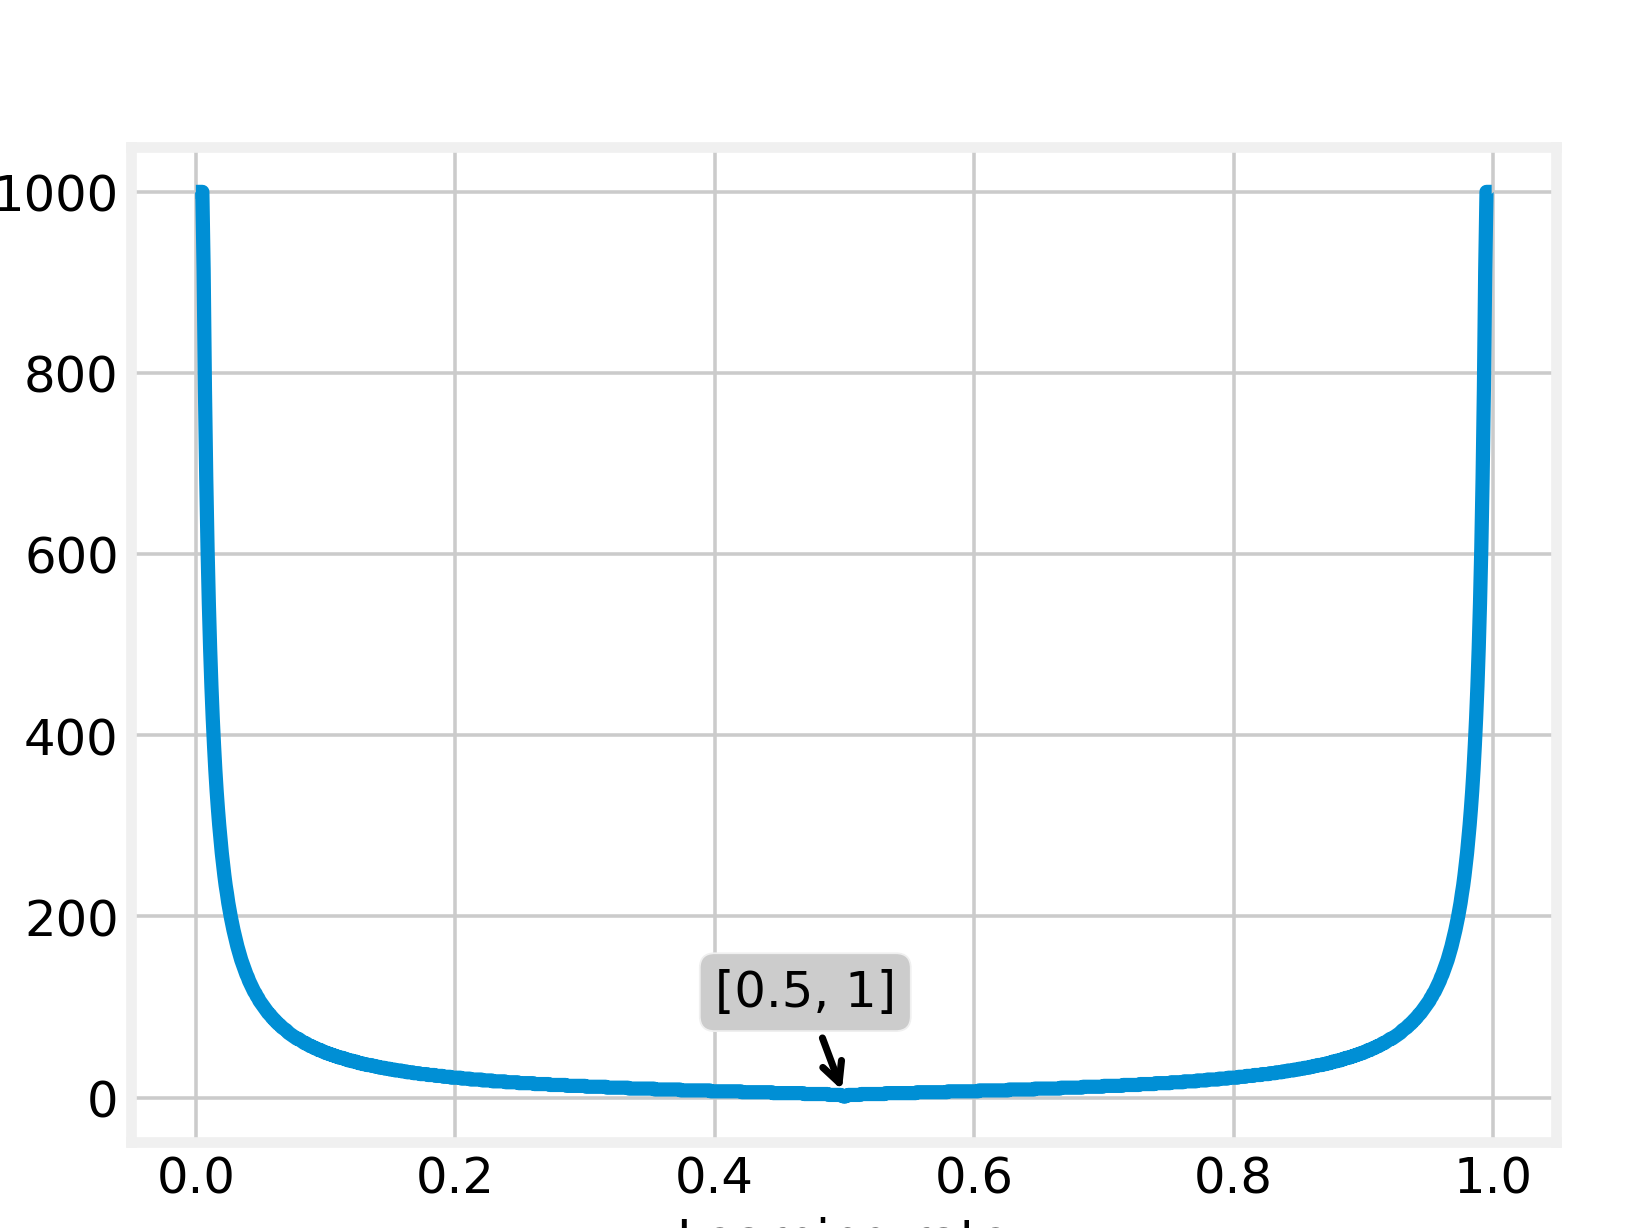
\includegraphics[scale=0.68]{Image/T4_A_F1_constant_research_lr.png}
		\caption*{\texttt{T4\_A\_F1\_constant\_research\_lr}}
	\end{figure}
	Полученный результат $\langle 0.5, ~ 1 \rangle$, где первый аргумент это~-- это оптимальный шаг, при котором сделано минимальное число шагов, второй же~-- это количество шагов. Подытожим, при выборе функции крайне важно выбирать длину шага, так как любое изменение может привести к долгим ожиданиям (например, в окрестности $learning~rate = 1$).
	\subsubsection*{Пример 2}
	А теперь на менее очевидную вторую функцию, которая, напомним, выглядит так:
	\[
		f(x, y) = 0.7464451039232642 \cdot x^{2} + 0.637923954128351 \cdot x \cdot y + 0.5415655721418664 \cdot y^{2}
	\]
	Установим здесь те же начальные значения, только начальной точкой мы зададим $\langle 50, ~ -75 \rangle$, а предельным числом шагов зададим в $1000$, ибо, по техническим причинам, слишком большие значения приводит к длительным вычислениям.
	\begin{figure}[H]
		\centering
		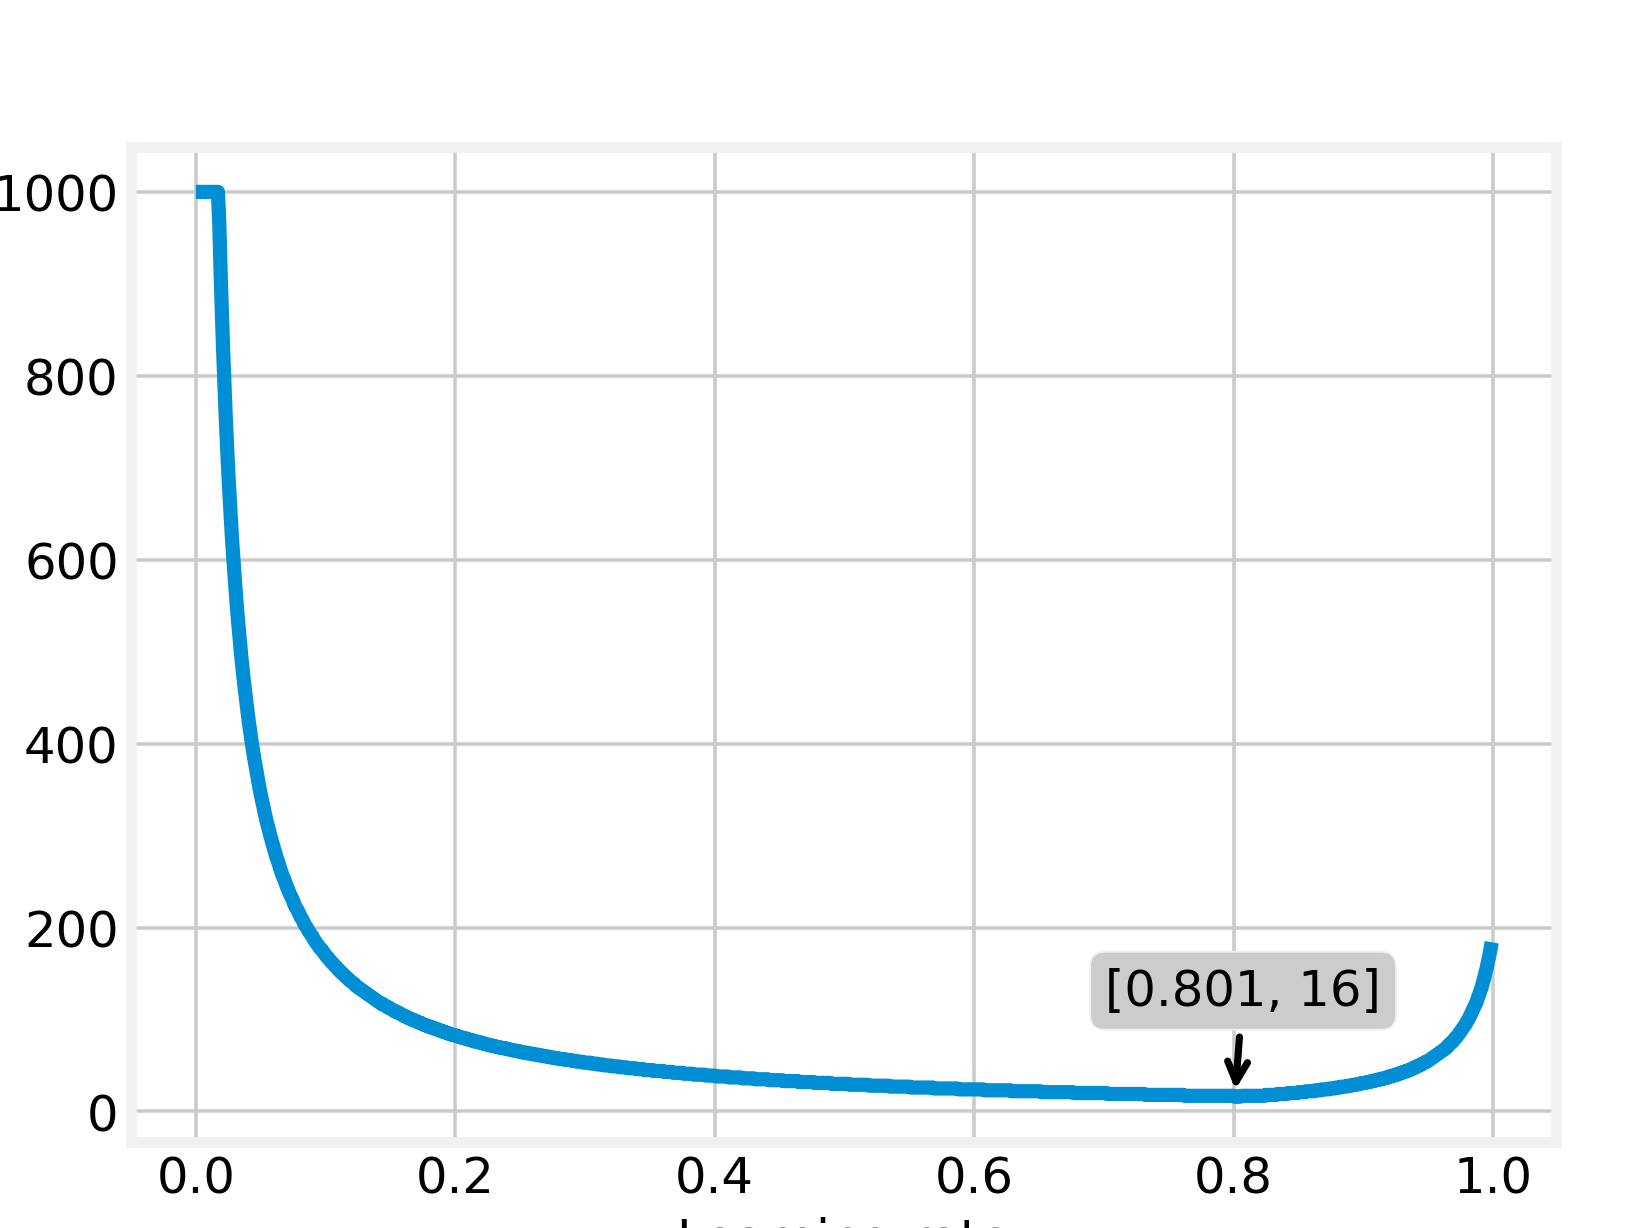
\includegraphics[scale=0.68]{Image/T4_A_F2_constant_research_lr.png}
		\caption*{\texttt{T4\_A\_F2\_constant\_research\_lr}}
	\end{figure}
	Здесь более интересные результаты. Мы получили почти параболу, у которой минимум находится в точке $0.801$, где было сделано алгоритмом минимальное число шагов.
	\subsection*{Решение пункта (b)}
	\subsubsection*{Пример 1}
	Теперь нам хотелось бы посмотреть на количество шагов, проводимыми обоими методами спуска к минимуму, то есть количество вызовов функции $f(x)$ для подсчета. Возьмем функцию $f(x, y) = x^{2} + y^{2}$ и взглянем на две величины~-- постоянный шаг, который имеет такой же диапазон и шаг изменения, и количество вызовов настоящей функции. Начальные точки такие же, как в прошлом.
	\begin{figure}[H]
		\centering
		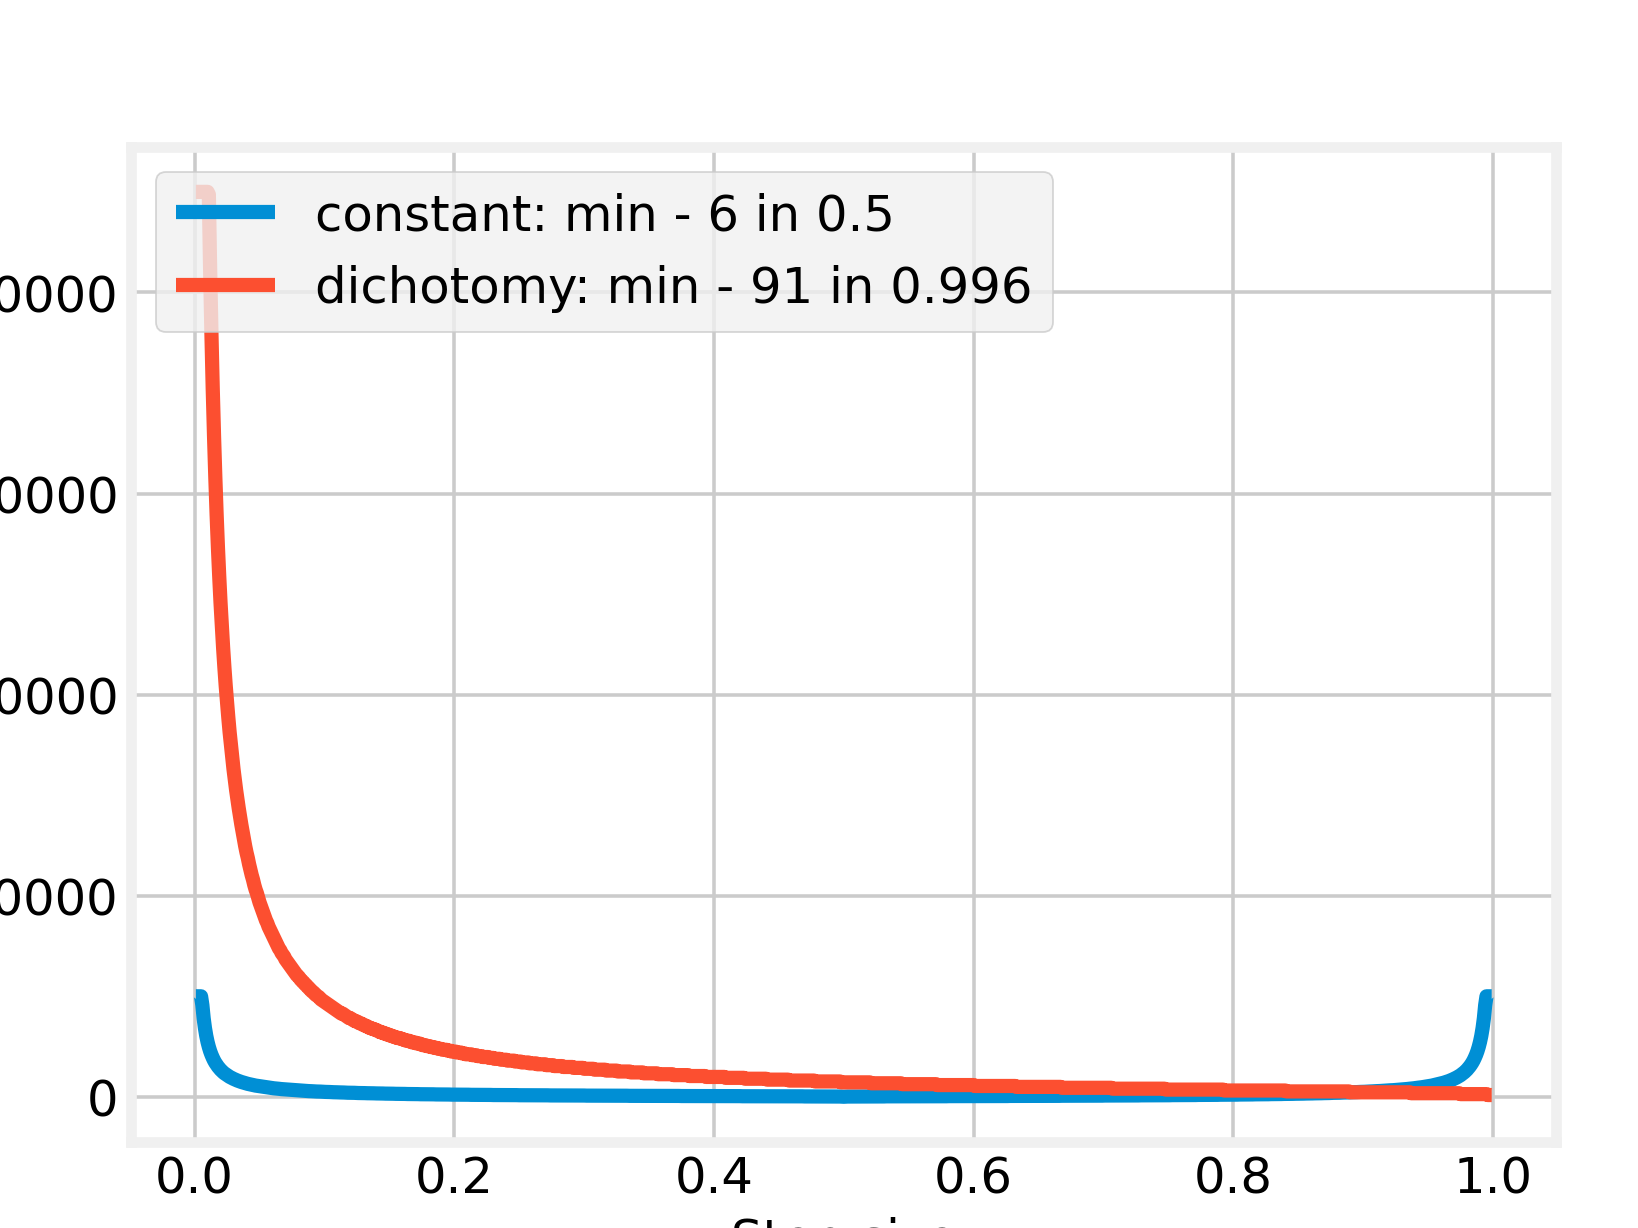
\includegraphics[scale=0.68]{Image/T4_B_F1_line_search_and_constant_research_step_size.png}
		\caption*{\texttt{T4\_B\_F1\_line\_search\_and\_constant\_research\_step\_size}}
	\end{figure}
	В среднем, дихотомия вызывает функцию большее количество раз, потому, как мы знаем, при выборе шага, смотрит на значение функции для выбора уменьшения шага.
	\subsubsection*{Пример 2}
	А теперь посмотрим на вторую функцию:
	\[
		f(x, y) = 0.7464451039232642 \cdot x^{2} + 0.637923954128351 \cdot x \cdot y + 0.5415655721418664 \cdot y^{2}
	\]
	Здесь мы устанавливаем такие же значения, что и в прошлом пункте. Посмотрим на полученный результат:
	\begin{figure}[H]
		\centering
		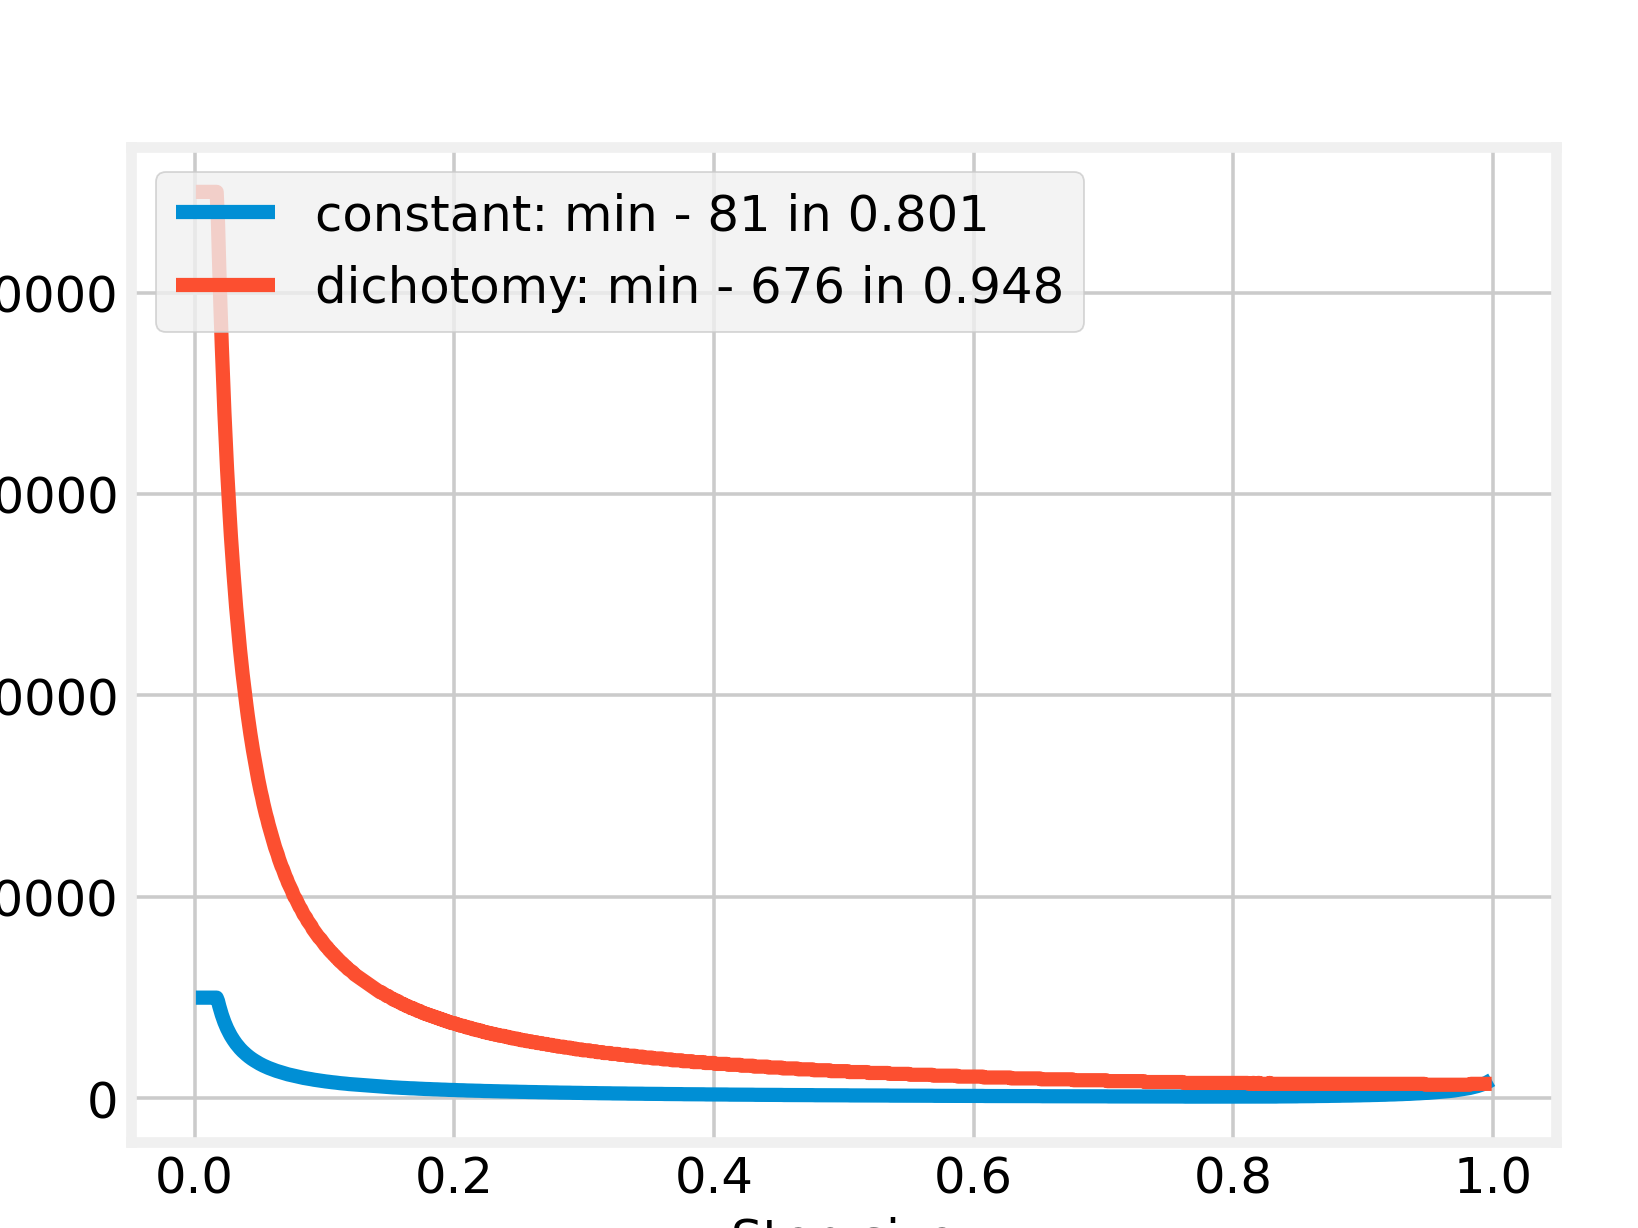
\includegraphics[scale=0.68]{Image/T4_B_F2_line_search_and_constant_research_step_size.png}
		\caption*{\texttt{T4\_B\_F2\_line\_search\_and\_constant\_research\_step\_size}}
	\end{figure}
	Как и в прошлом пункте мы получаем такое же поведение дихотомии: этот метод вызывает в среднем куда количество больше раз, чем стандартный, из-за метода выбора $scale$ для шага.
	\subsection*{Решение пункта (c)}
	\subsubsection*{Пример 1}
	Теперь хотим исследовать количество итераций алгоритма в зависимости от начальной точки. В качестве пространства мы выберем пространство $M \subset \mathbb{R}^{2}$ с максимальными и минимальными точками $80$ и $-80$ соответственно для каждой из осей. Сначала посмотрим на обычный градиентный спуск, установим $learning~rate$ для этого примера равным $0.05$ и максимальным количеством итераций в $1000$. Посмотрим на результат.
	\begin{figure}[H]
		\centering
		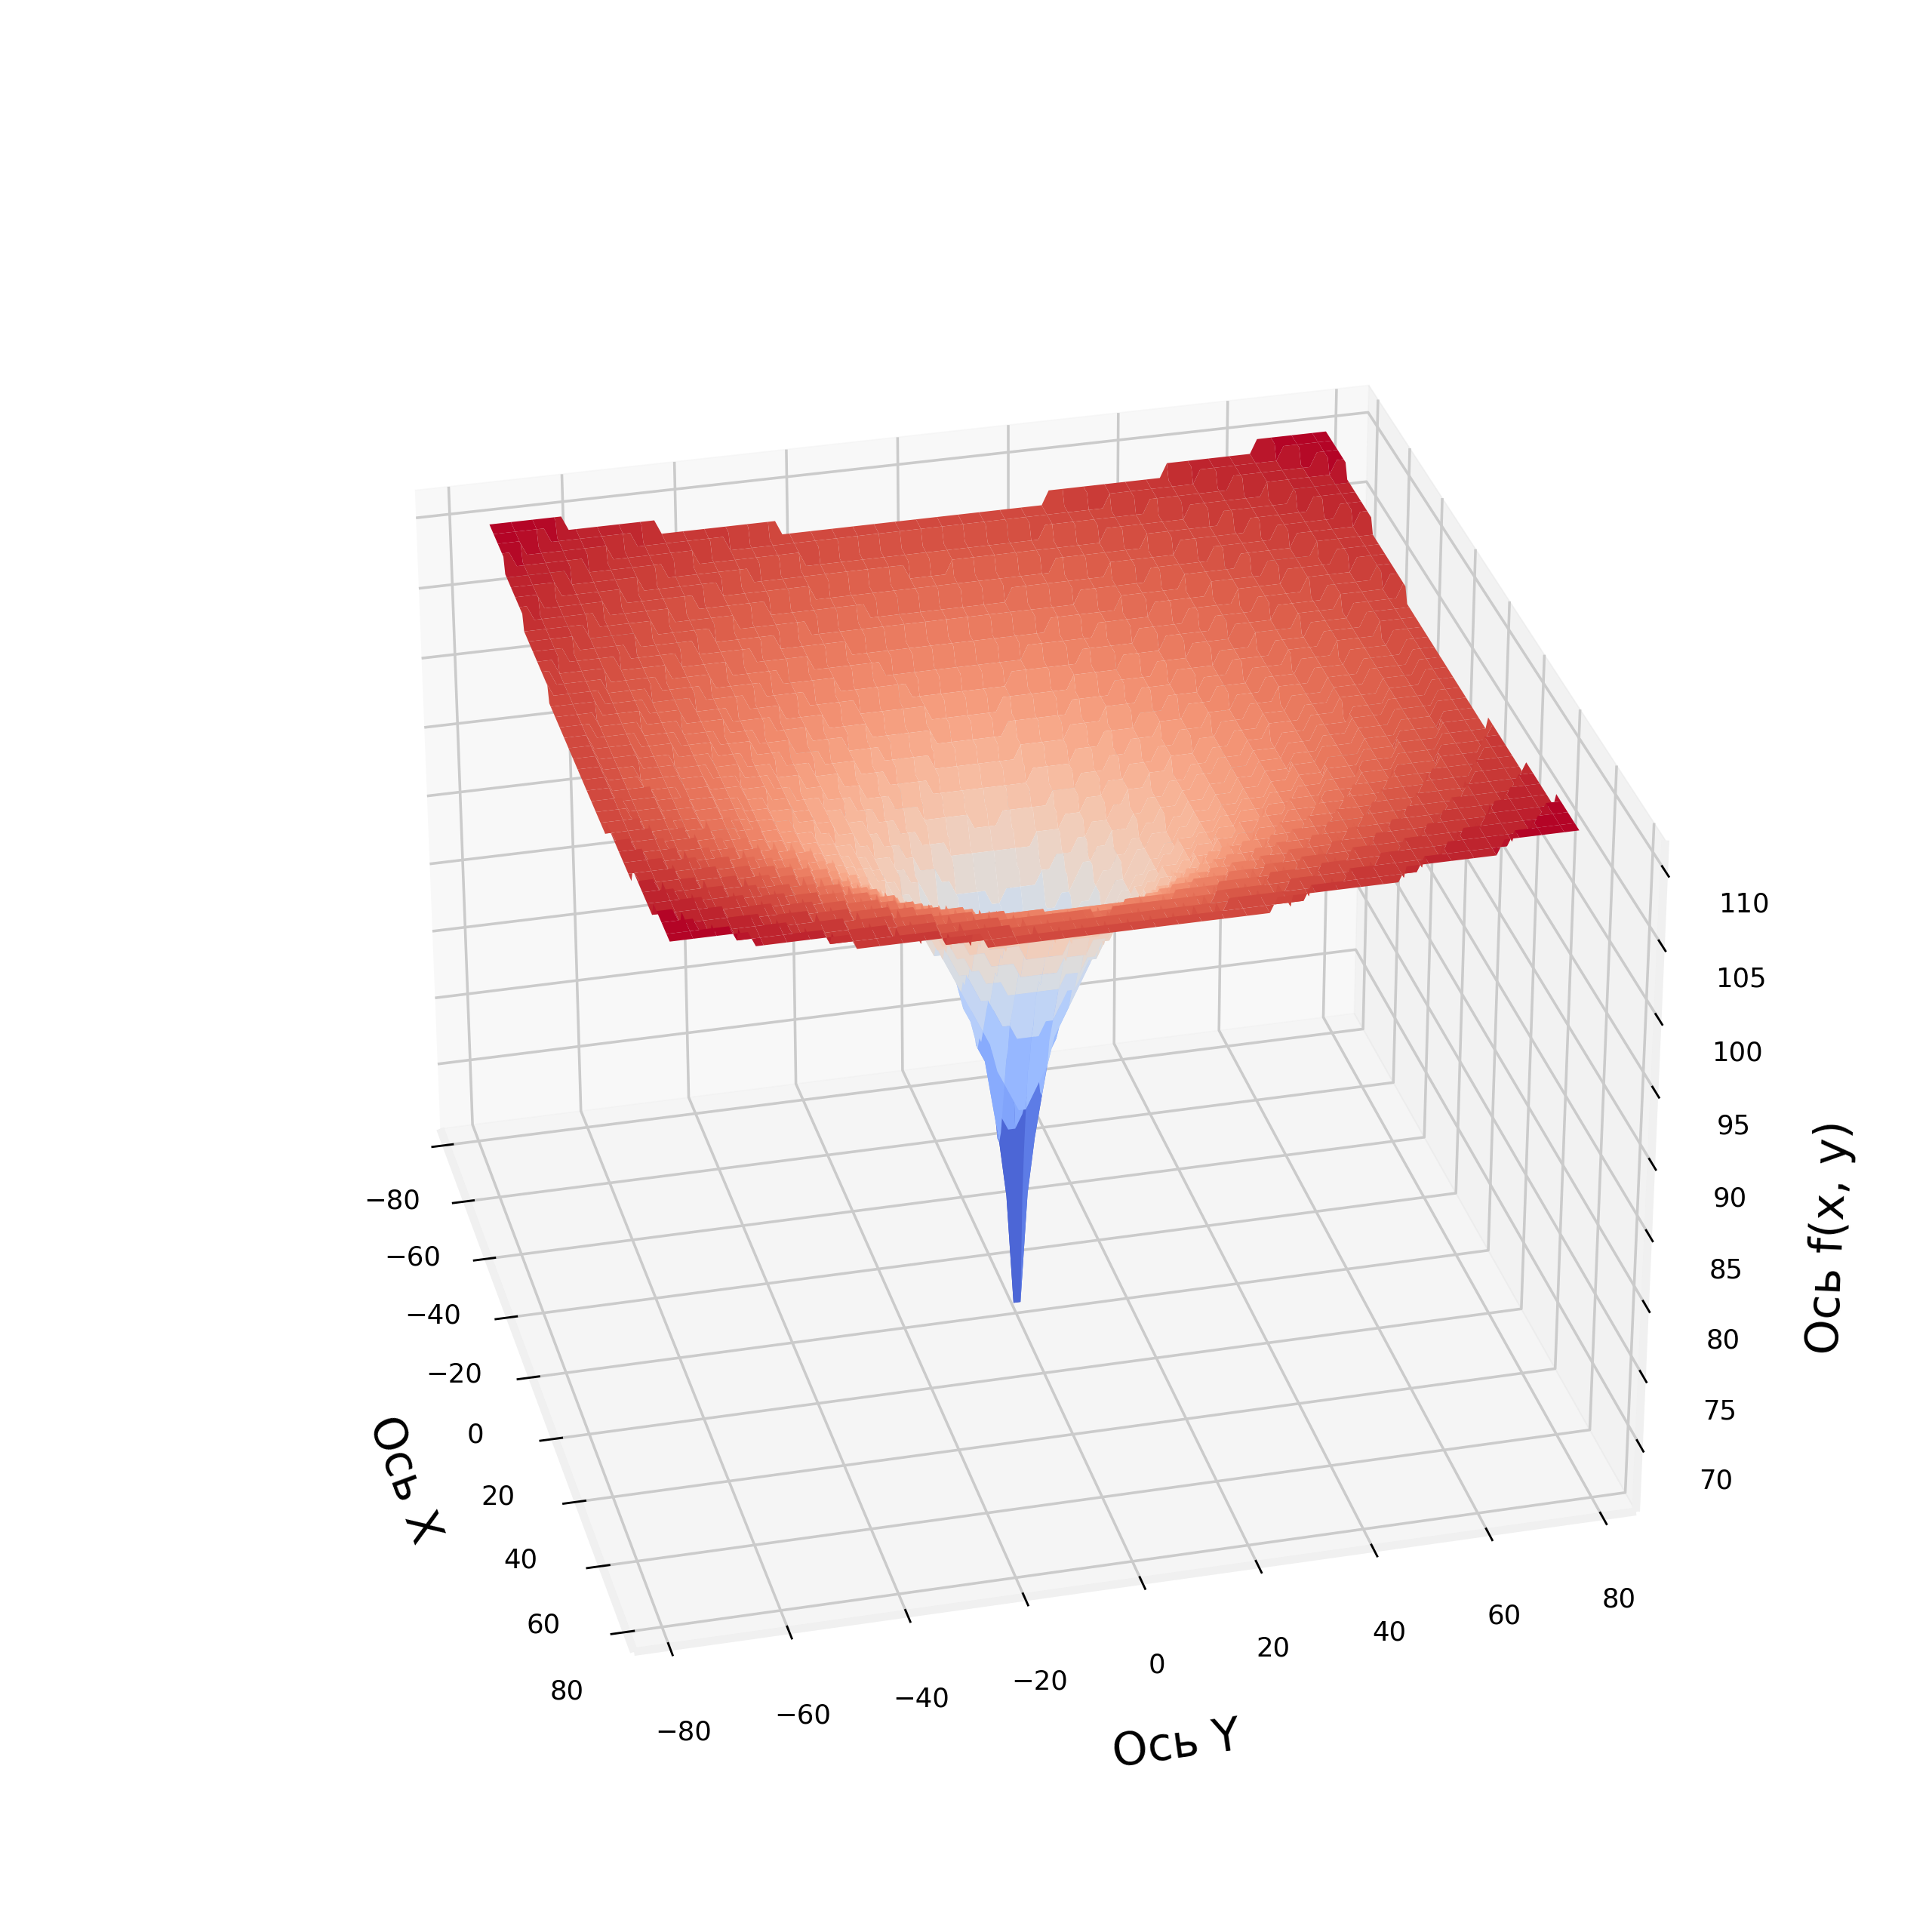
\includegraphics[scale=0.68]{Image/T4_C_F1_steps_dependens_on_start_point_constant.png}
		\caption*{\texttt{T4\_C\_F1\_steps\_dependens\_on\_start\_point\_constant}}
	\end{figure}
	У нас образовалась аккуратная <<яма>>, которая впадает в почти середину всего заданного пространства. Объяснение гладкости можно привести такое: это значит, что при небольшом изменении $\langle x, ~ y\rangle \to \langle x + \delta, ~ y + \lambda \rangle$ количество итерация на обычным спуске изменяется понемногу. Затем, уже ближе к минимуму функции, функция становится более грубой, за счет градиента <<падения>> к минимуму функции. А теперь посмотрим на вариант с дихотомией, с шагом в $0.5$ и таким же количеством итераций максимально:
	\begin{figure}[H]
		\centering
		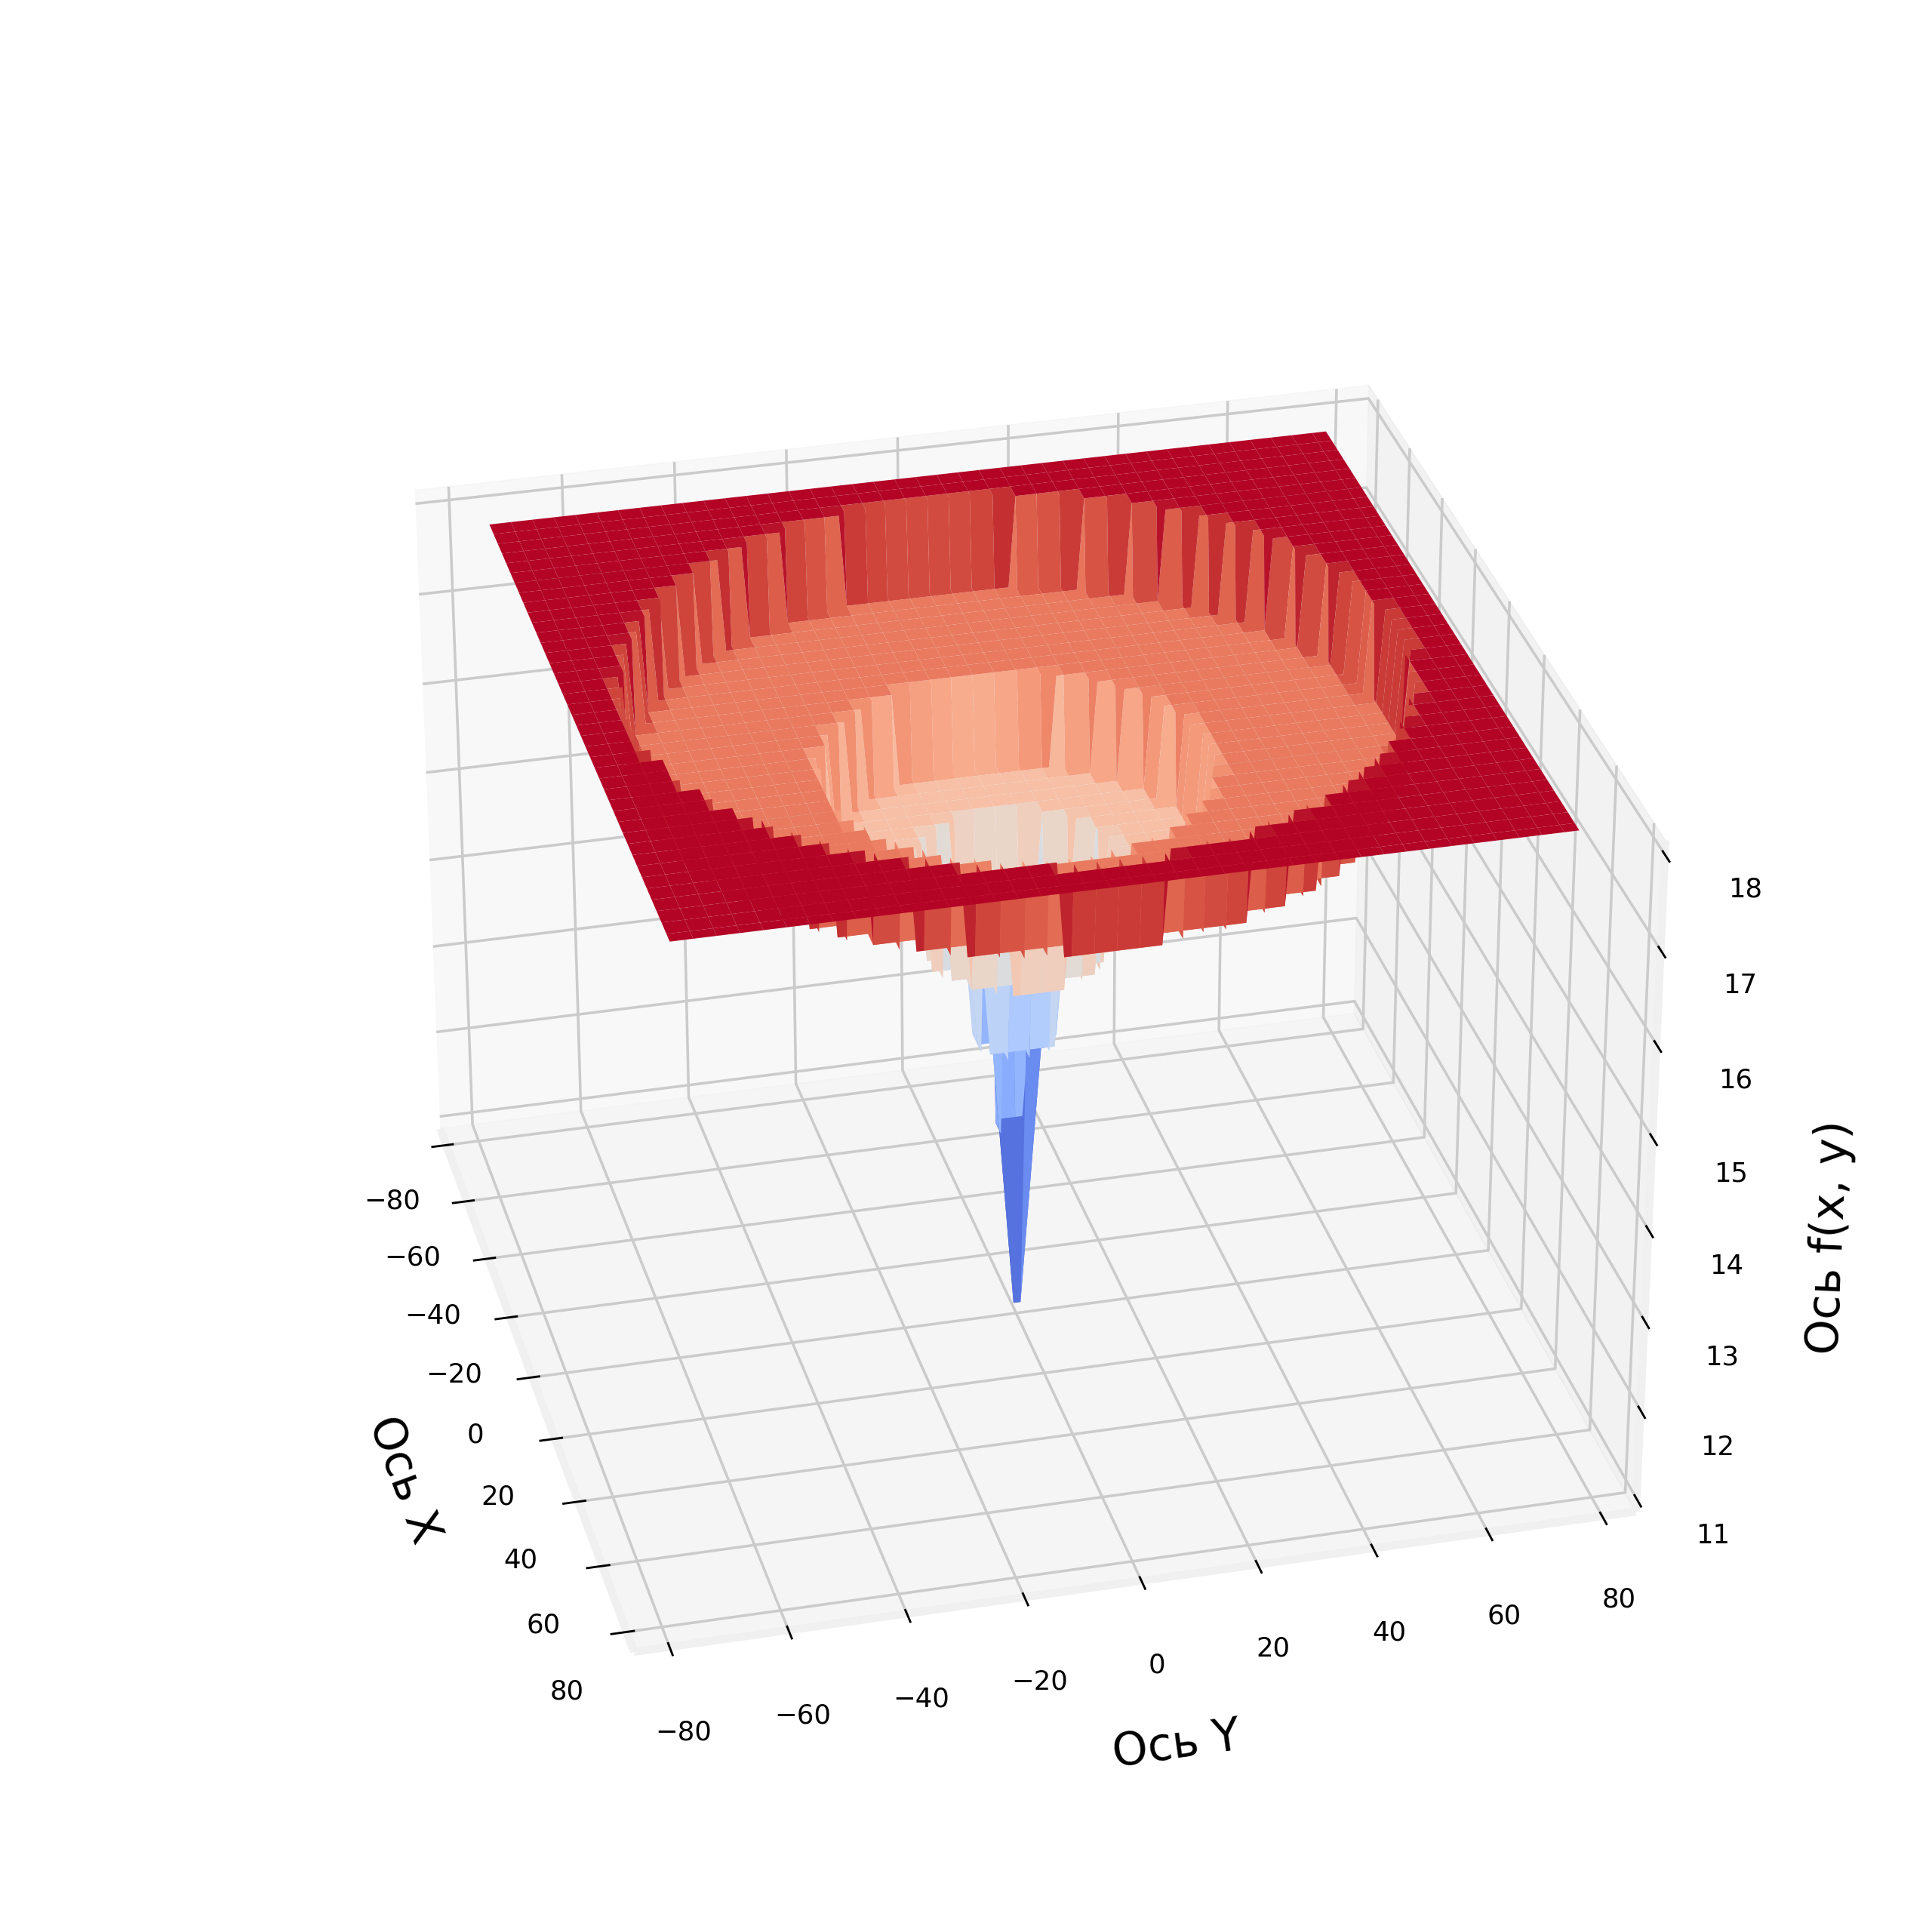
\includegraphics[scale=0.68]{Image/T4_C_F1_steps_dependens_on_start_point_dichotomy.png}
		\caption*{\texttt{T4\_C\_F1\_steps\_dependens\_on\_start\_point\_dichotomy}}
	\end{figure}
	Теперь <<яма>> более грубая и имеет резкие падения вниз в некоторых точках, при этом такая ситуация возникает как бы по слоям~-- такое происходит из-за выборности $scale$, как только спуск находит необходимый шаг - он тут же туда <<прыгает>>.
	\subsubsection*{Пример 2}
	А теперь проделаем те же действия, что и ранее, только с функцией $f(x, y)$, заданной следующим образом:
	\[
		f(x, y) = 0.7464451039232642 \cdot x^{2} + 0.637923954128351 \cdot x \cdot y + 0.5415655721418664 \cdot y^{2}
	\]
	Установим на алгоритмы те же параметры, что и прежде, то есть,
	\begin{itemize}
		\item градиентный спуск~-- длина шаг остается $0.05$, максимальное число итераций~-- $1000$;
		\item тот же с методом дихотомии~-- длина в $0.5$, максимальное число~-- всё также $1000$.
	\end{itemize}
	Посмотрим сначала на градиентный спуск.
	\begin{figure}[H]
		\centering
		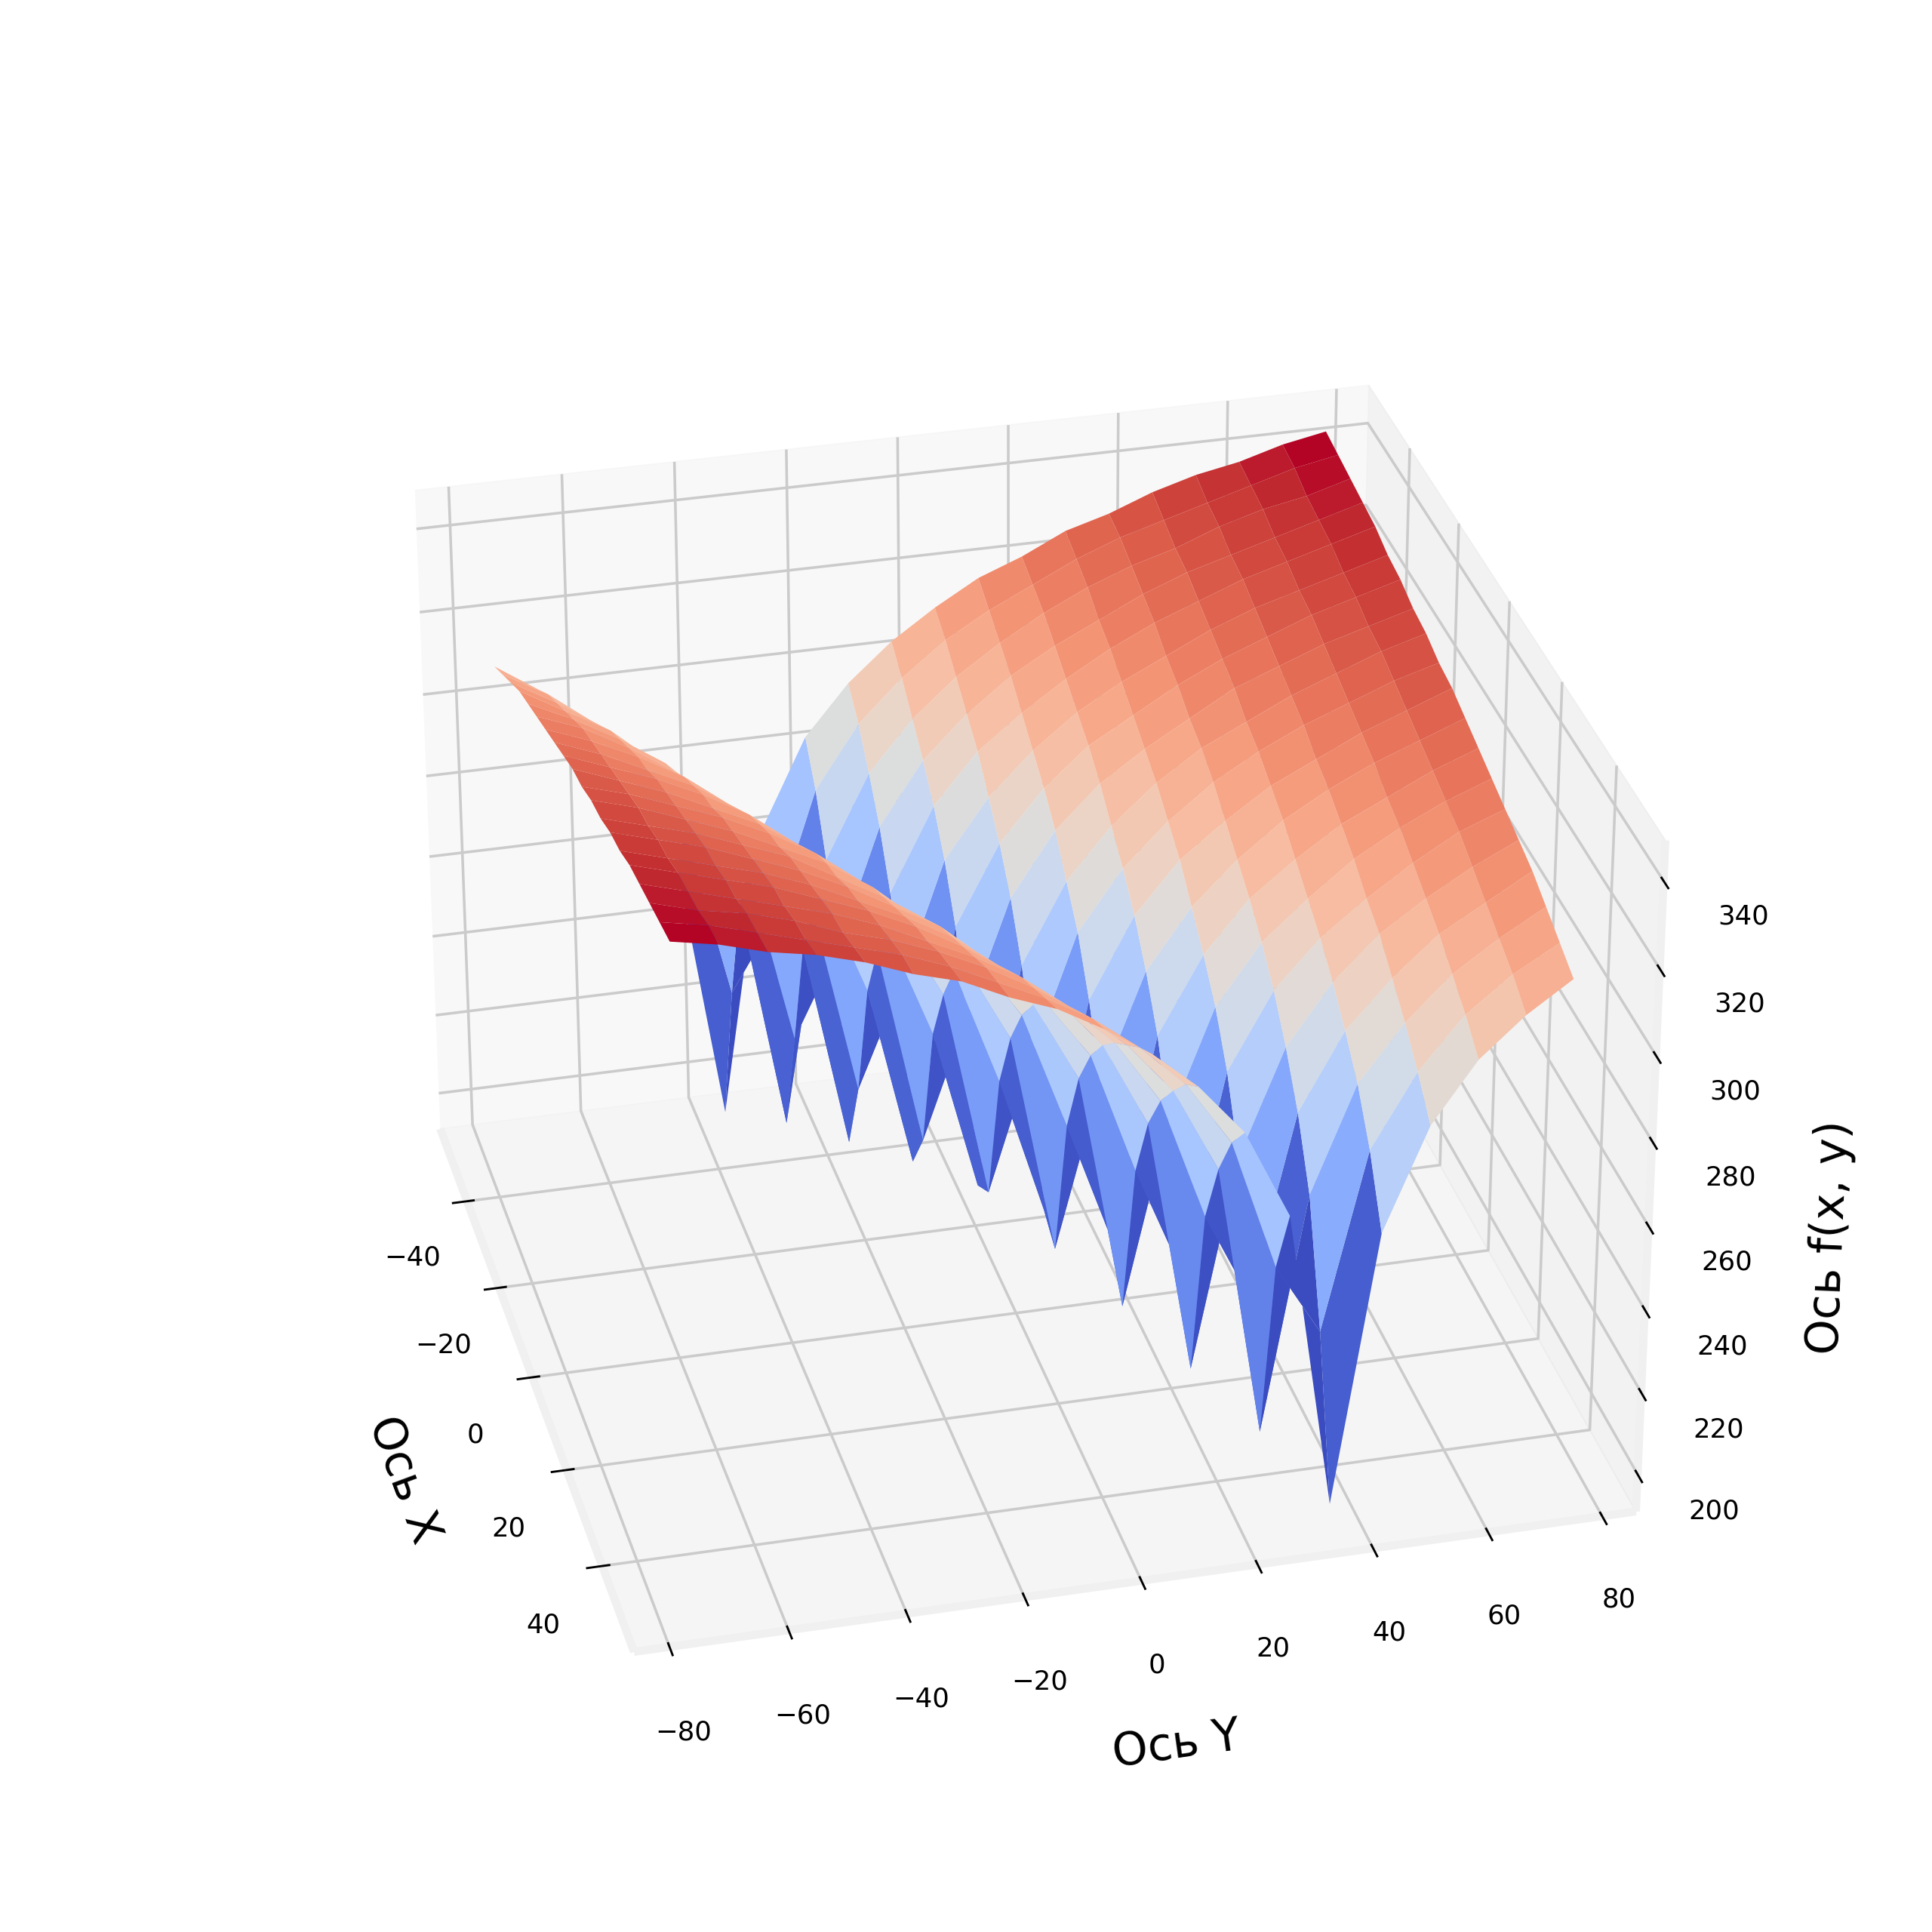
\includegraphics[scale=0.68]{Image/T4_C_F2_steps_dependens_on_start_point_constant.png}
		\caption*{\texttt{T4\_C\_F2\_steps\_dependens\_on\_start\_point\_constant}}
	\end{figure}
	Получаем ровно ту же ситуацию, что и с первым примером, что интересно: вновь гладкая <<горка>> в минимум. Объяснение здесь опять же ровно такое: мы меняем значения с постоянным шагом, а значит, а значит с близостью начальной точки к минимуму будет меняться с константой величиной. Теперь рассмотрим дихотомию:
	\begin{figure}[H]
		\centering
		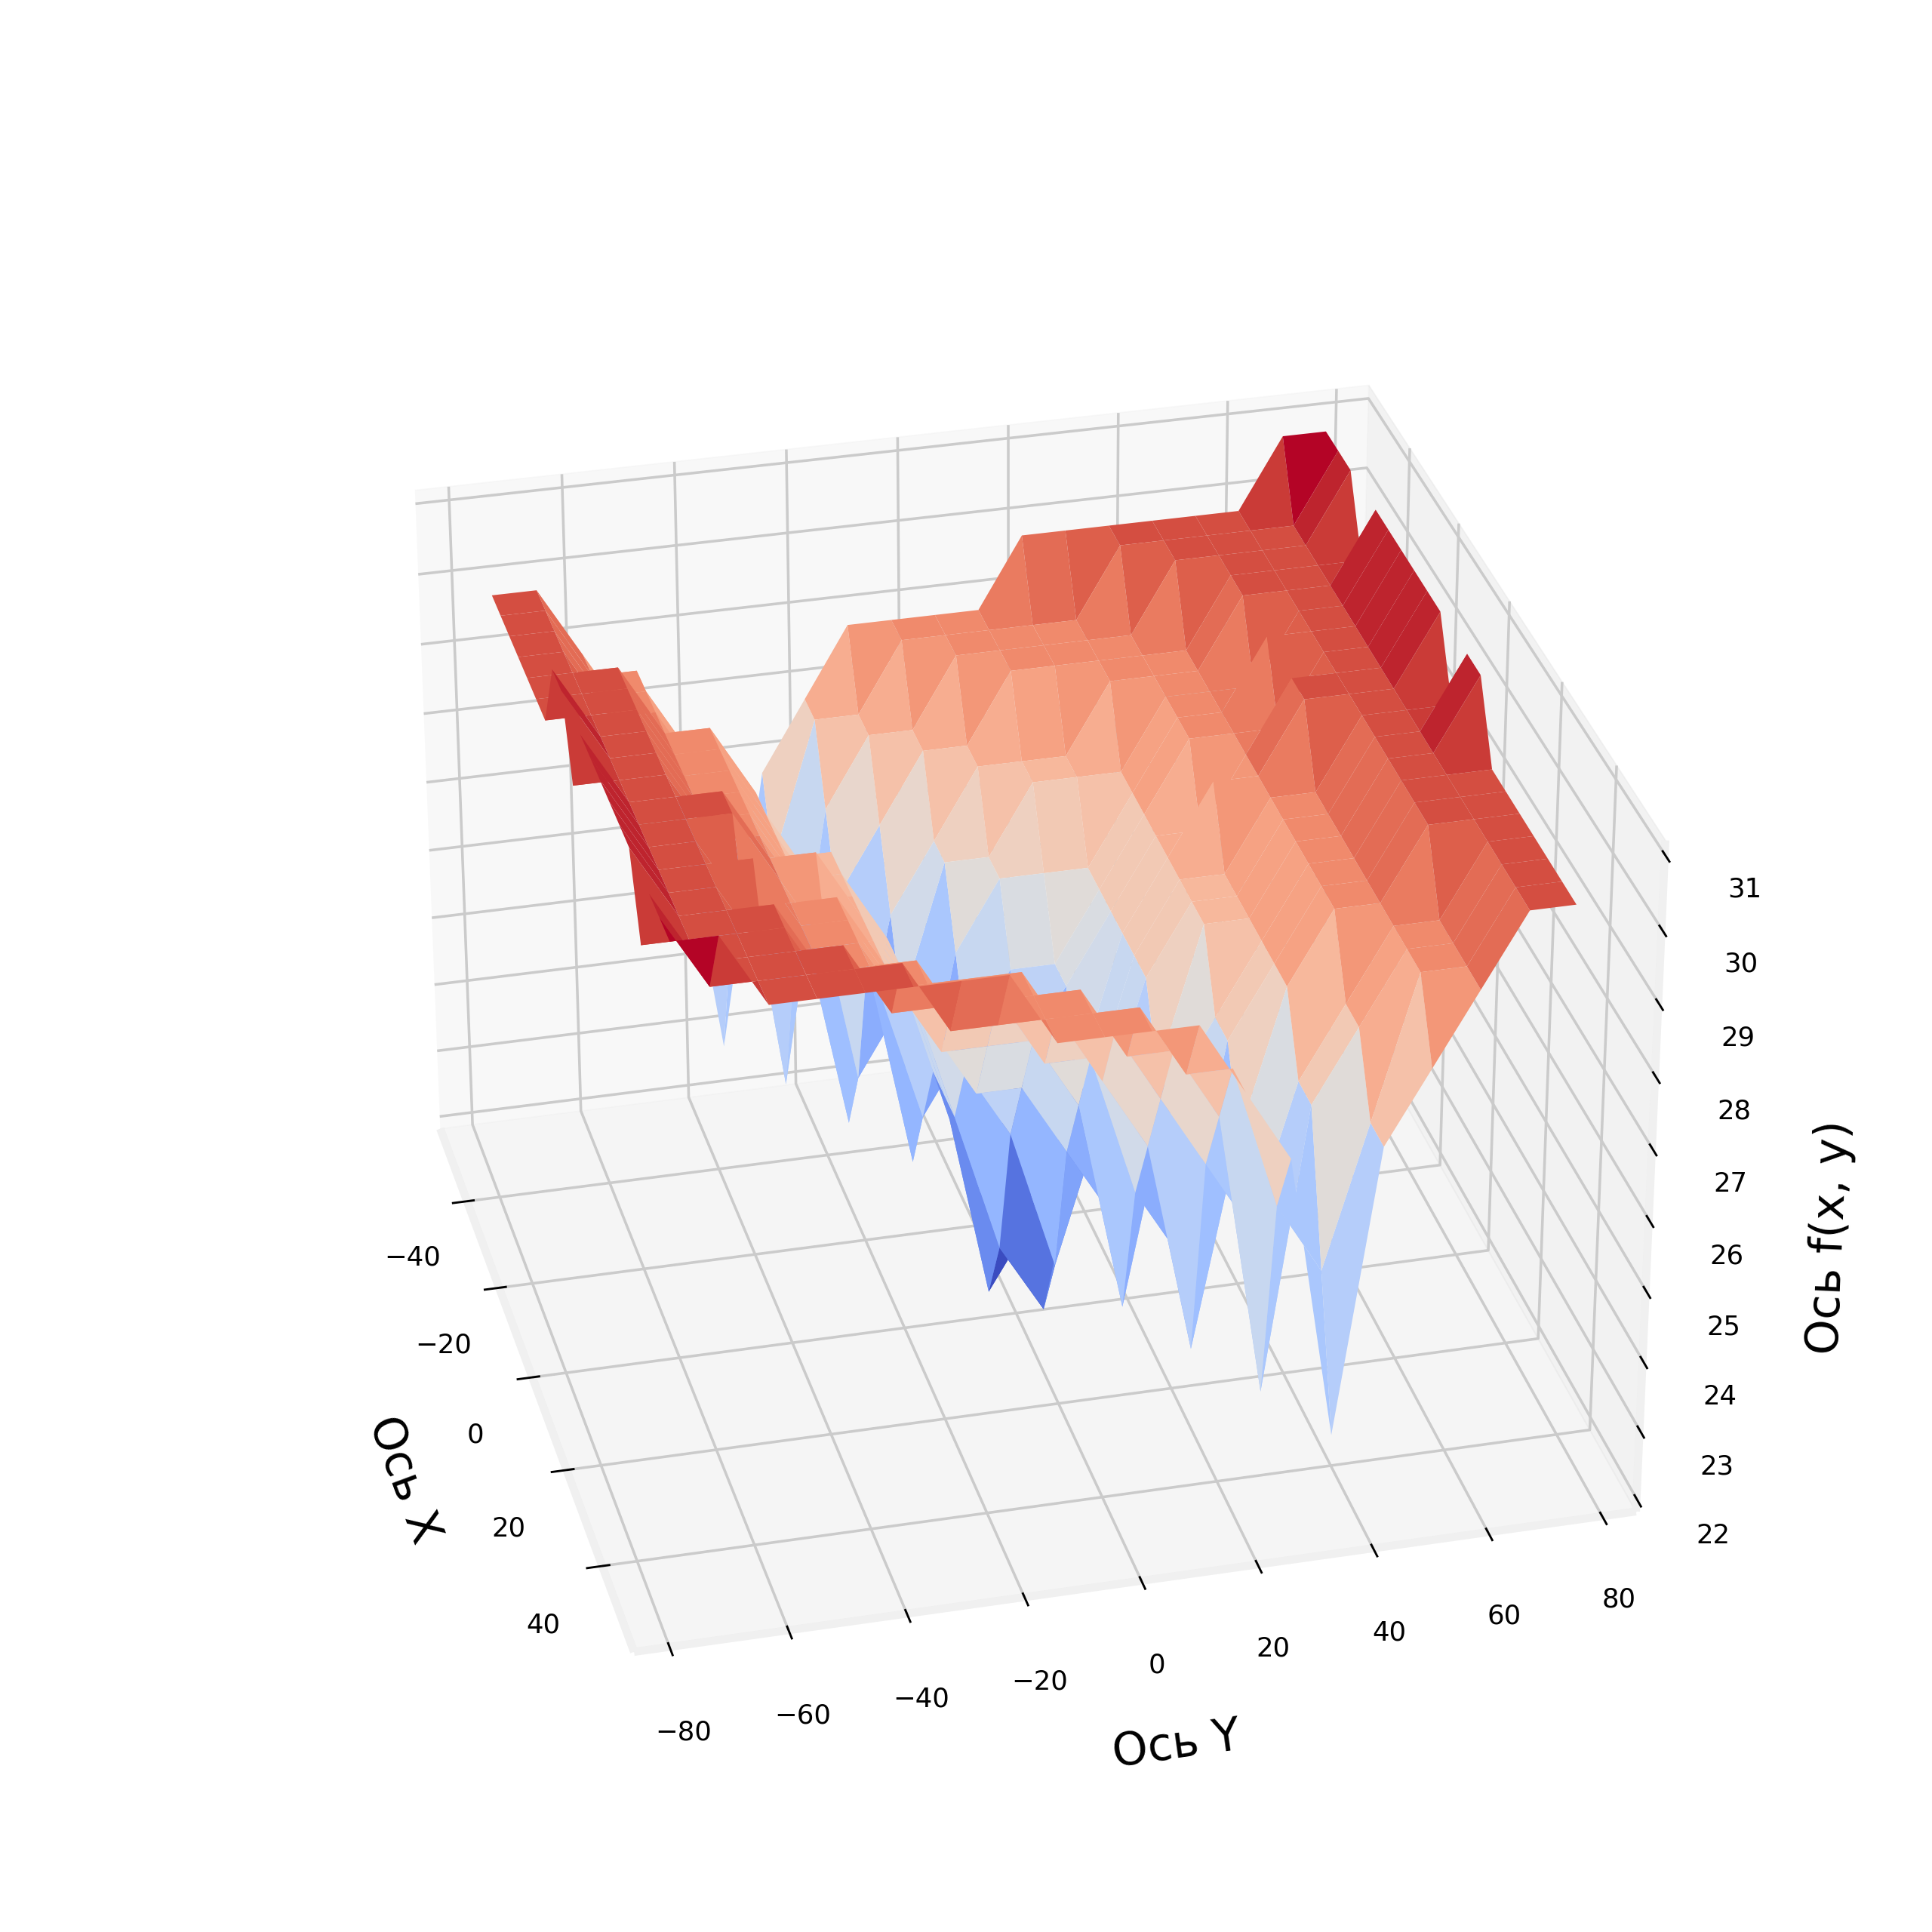
\includegraphics[scale=0.68]{Image/T4_C_F2_steps_dependens_on_start_point_dichotomy.png}
		\caption*{\texttt{T4\_C\_F2\_steps\_dependens\_on\_start\_point\_dichotomy}}
	\end{figure}
	Аналогичная ситуация с дихотомией и в прошлом пункте получаем более грубый график.
	\subsection*{Решение пункта (d)}
	Суть \textit{scaling}'а в том, что при изменении функции, её минимум остается прежним или же он меняется на некоторую константу. Мы рассматриваем квадратичные функции, а значит минимум будет один и тот же~-- $0$. В случае с градиентным спуском в случаи с растягиванием или сжатием функции количество шагов до приближенного минимума либо увеличится, либо уменьшится.

	Рассмотрим первую функцию $f(x, y) = x^2 + y^2$ и начнем проводить масштабирование в диапазоне $[0, 100]$ с шагом $0.1$ и ограничим число шагов алгоритма в $1000$. Тогда, посмотрим на результат:
	\begin{figure}[H]
		\centering
		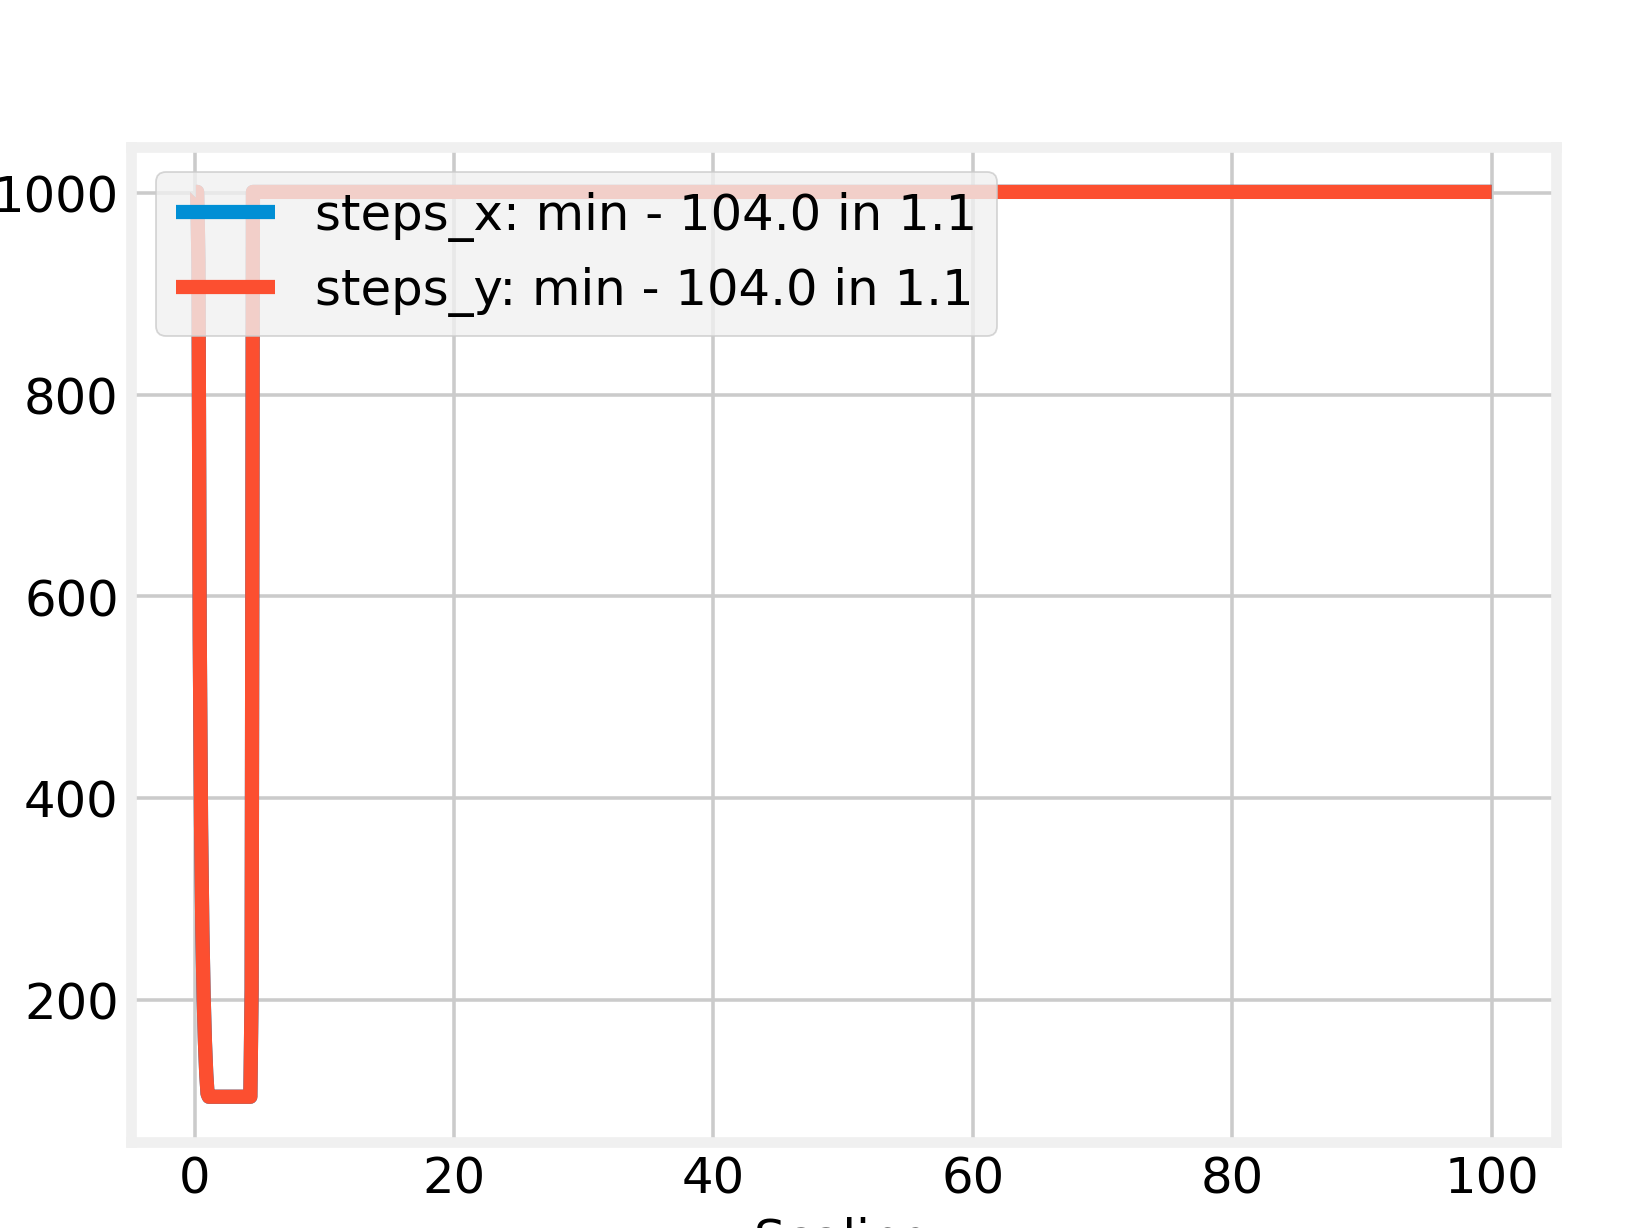
\includegraphics[scale=0.68]{Image/T4_D_F1_scaling_effect_constant.png}
		\caption*{\texttt{T4\_D\_F1\_scaling\_effect\_constant}}
	\end{figure}
	Очевидно, почему в районе $0$ мы получаем резкое возрастание числа шагов, потому что у нас остается одна ось, в которой точка никуда не движется и мы получаем длительный цикл для схождения второй оси к нулю, потому-что $learning~rate$ больше чем заданный $scaling$. Во всех остальных значениях, в пределах $(0, 5 \pm \varepsilon)$ мы получаем, наоборот, минимальное число шагов за счет более <<удачного>> масштабировании с одной и той же начальной точкой. Как промежуточный итог: масштабирование может увеличить эффективность работы алгоритма.

	Только что мы рассмотрели случай с обычный градиентным спуском. А теперь посмотрим на тот же метод, но на основе метода дихотомии.
	\begin{figure}[H]
		\centering
		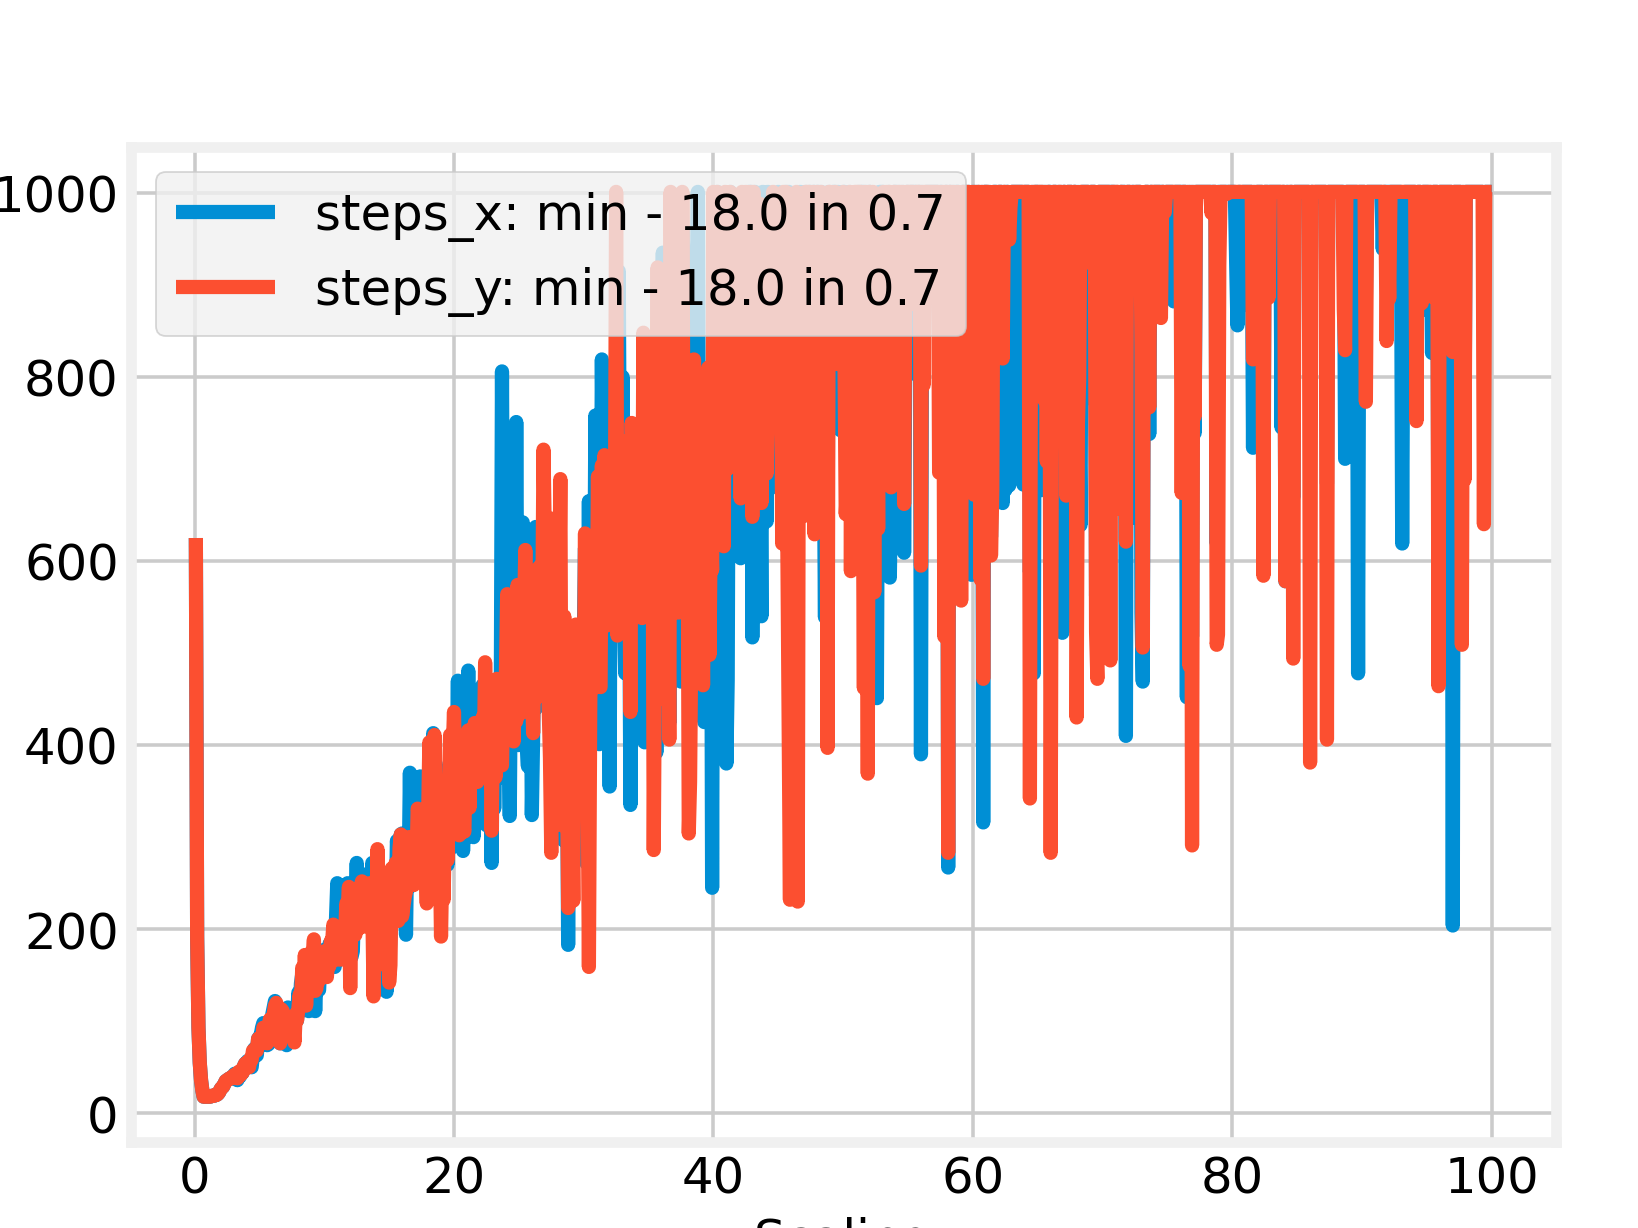
\includegraphics[scale=0.68]{Image/T4_D_F1_scaling_effect_dichotomy.png}
		\caption*{\texttt{T4\_D\_F1\_scaling\_effect\_dichotomy}}
	\end{figure}
	Здесь сильно ситуация отличается от константного случая. Заметим, что изменение, что у $x$, что $y$ дают разные результаты поведения эффективности алгоритма. В районе нуля мы получаем вновь резкое возрастание, так как слишком маленькие задан $step\_size$ для алгоритма, однако в окрестности уже единицы, а именно при $0.7$, мы получаем возрастание эффективности алгоритма во многу раз для одной и той же начальной точки. Не забываем, что метод дихотомии, в отличии от константного случая, может в самом конце уменьшить свой шаг к минимуму. Как промежуточный итог: в случае с дихотомией мы получаем почти линейную зависимость.

	Теперь рассмотрим вторую функцию $f(x, y)$, которая выглядит так:
	\[
		f(x, y) = 0.7464451039232642 \cdot x^{2} + 0.637923954128351 \cdot x \cdot y + 0.5415655721418664 \cdot y^{2}
	\]
	Также рассмотрим сначала константный случай.
	\begin{figure}[H]
		\centering
		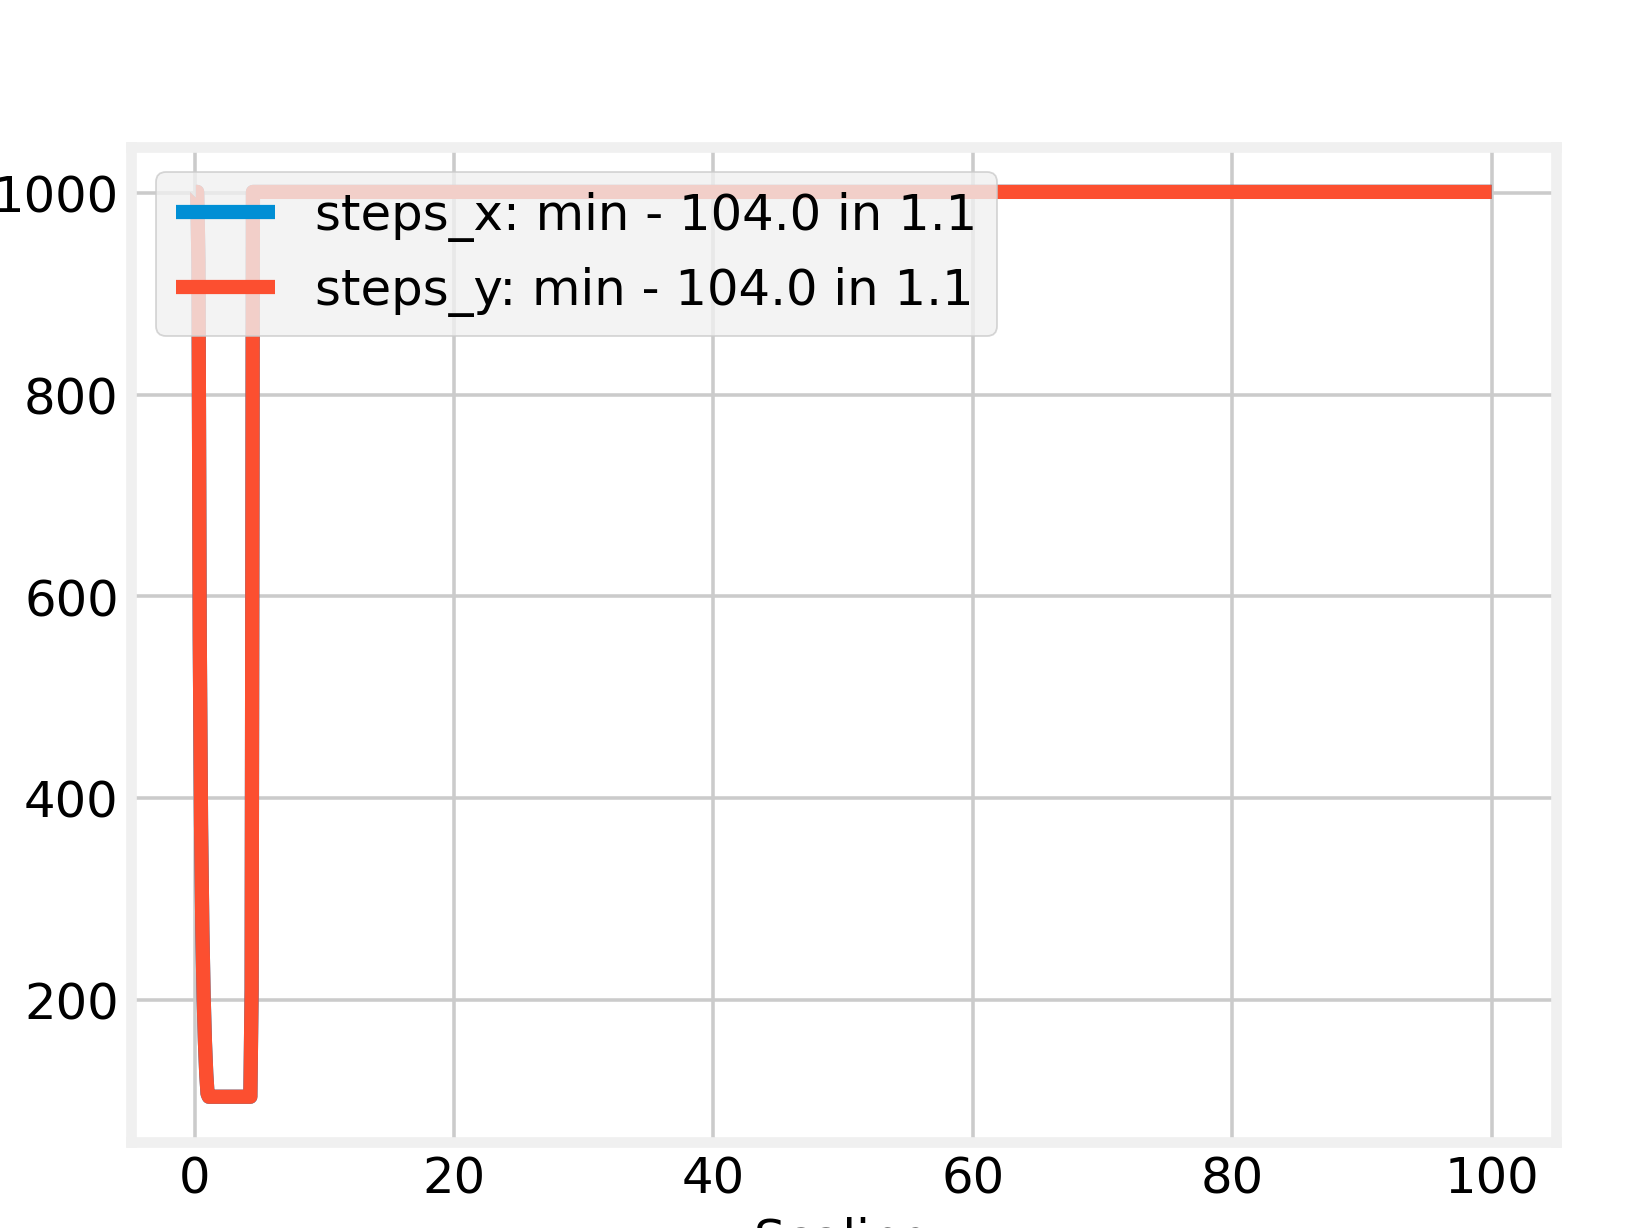
\includegraphics[scale=0.68]{Image/T4_D_F2_scaling_effect_constant.png}
		\caption*{\texttt{T4\_D\_F2\_scaling\_effect\_constant}}
	\end{figure}
	Неудивительно, что мы получили почти такой же график, что и для первой функции. Заметим, что количество шагов в районе нуля также сводится к большим значения, за счет большого $learning~rate$ и коэффициента при одной из осей.

	Рассмотрим теперь при методе дихотомии.
	\begin{figure}[H]
		\centering
		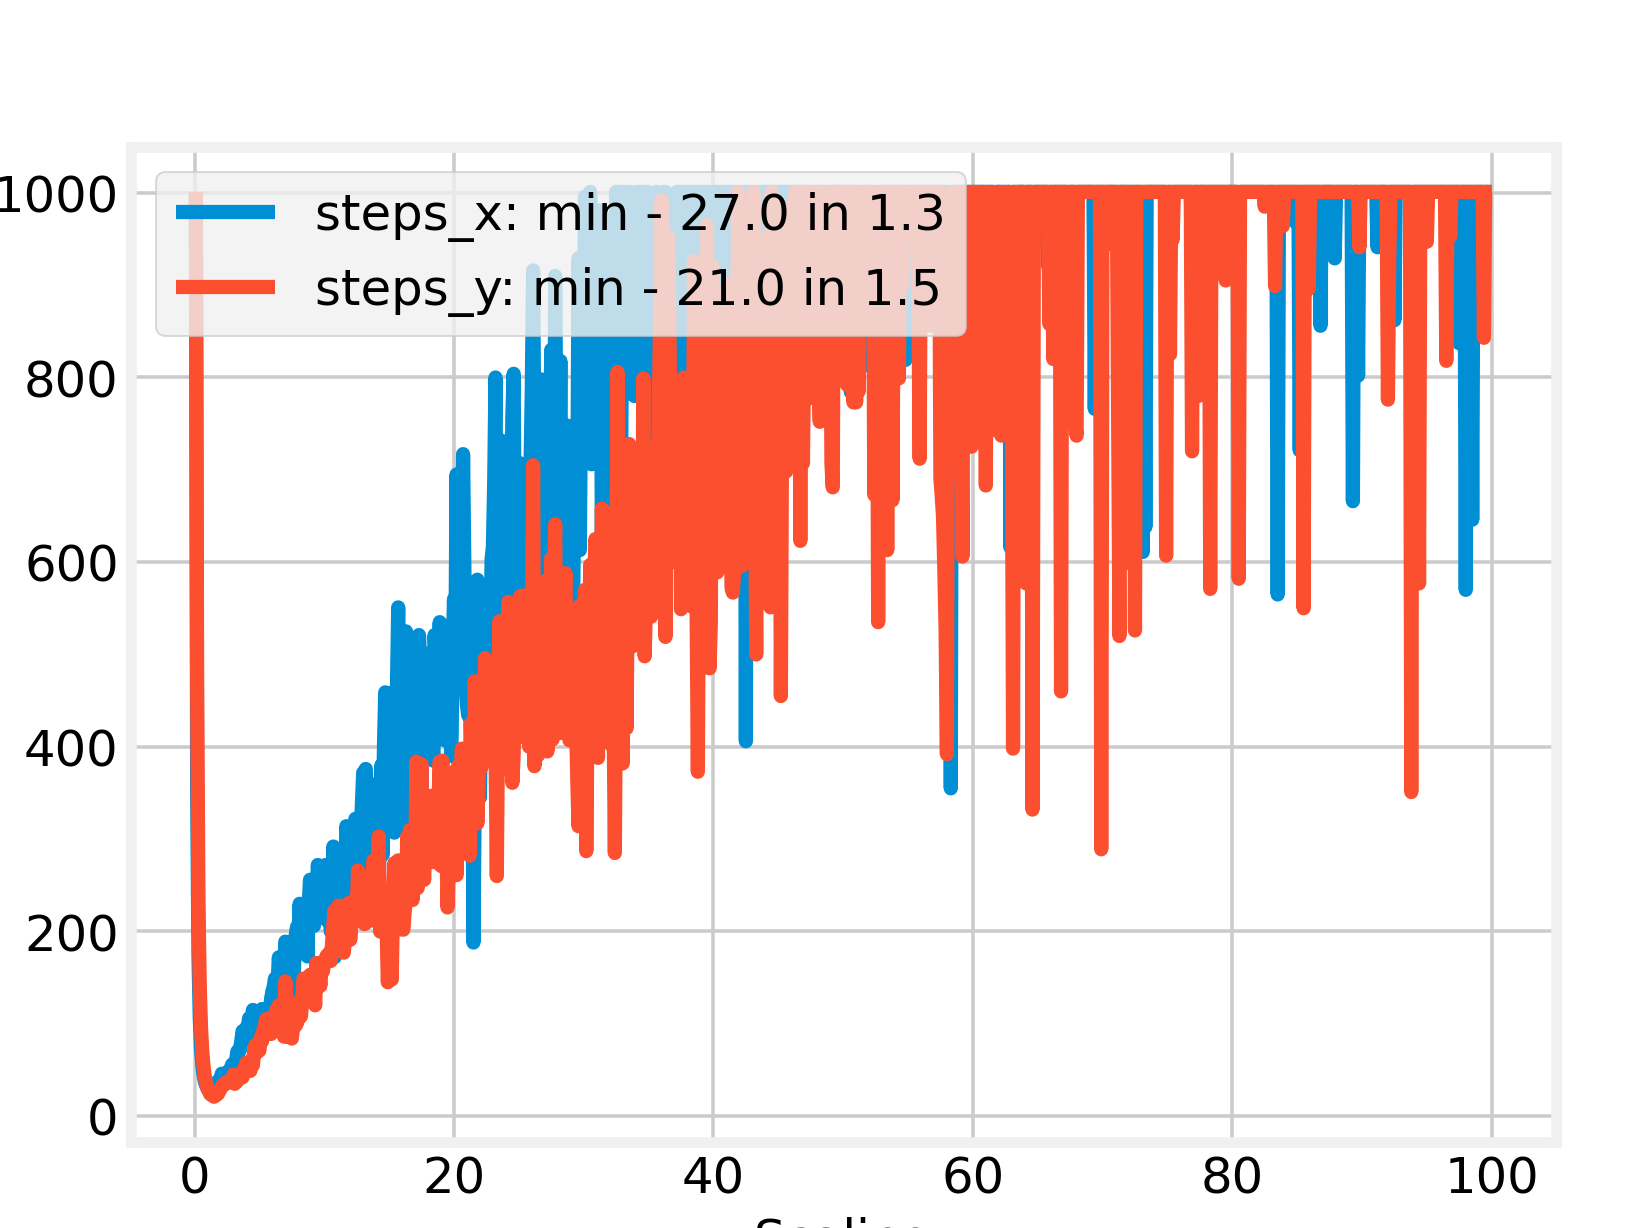
\includegraphics[scale=0.68]{Image/T4_D_F2_scaling_effect_dichotomy.png}
		\caption*{\texttt{T4\_D\_F2\_scaling\_effect\_dichotomy}}
	\end{figure}
	На графике мы видим, что при растягивании~-- мы получаем почти всю ту же линейную зависимость. Правда, на сей раз, коэффициент при $x^2$ уменьшает эффективность и количество шагов за счет большего коэффициента, чем у $y^2$, поэтому при одном и том же $scaling$ по оси $y$ число шагов еще не превышает максимально заданное, а по $x$~-- превышает.
	\subsection*{Решение пункта (e)}
	\begin{center}
		\begin{figure}[H]
			\centering
			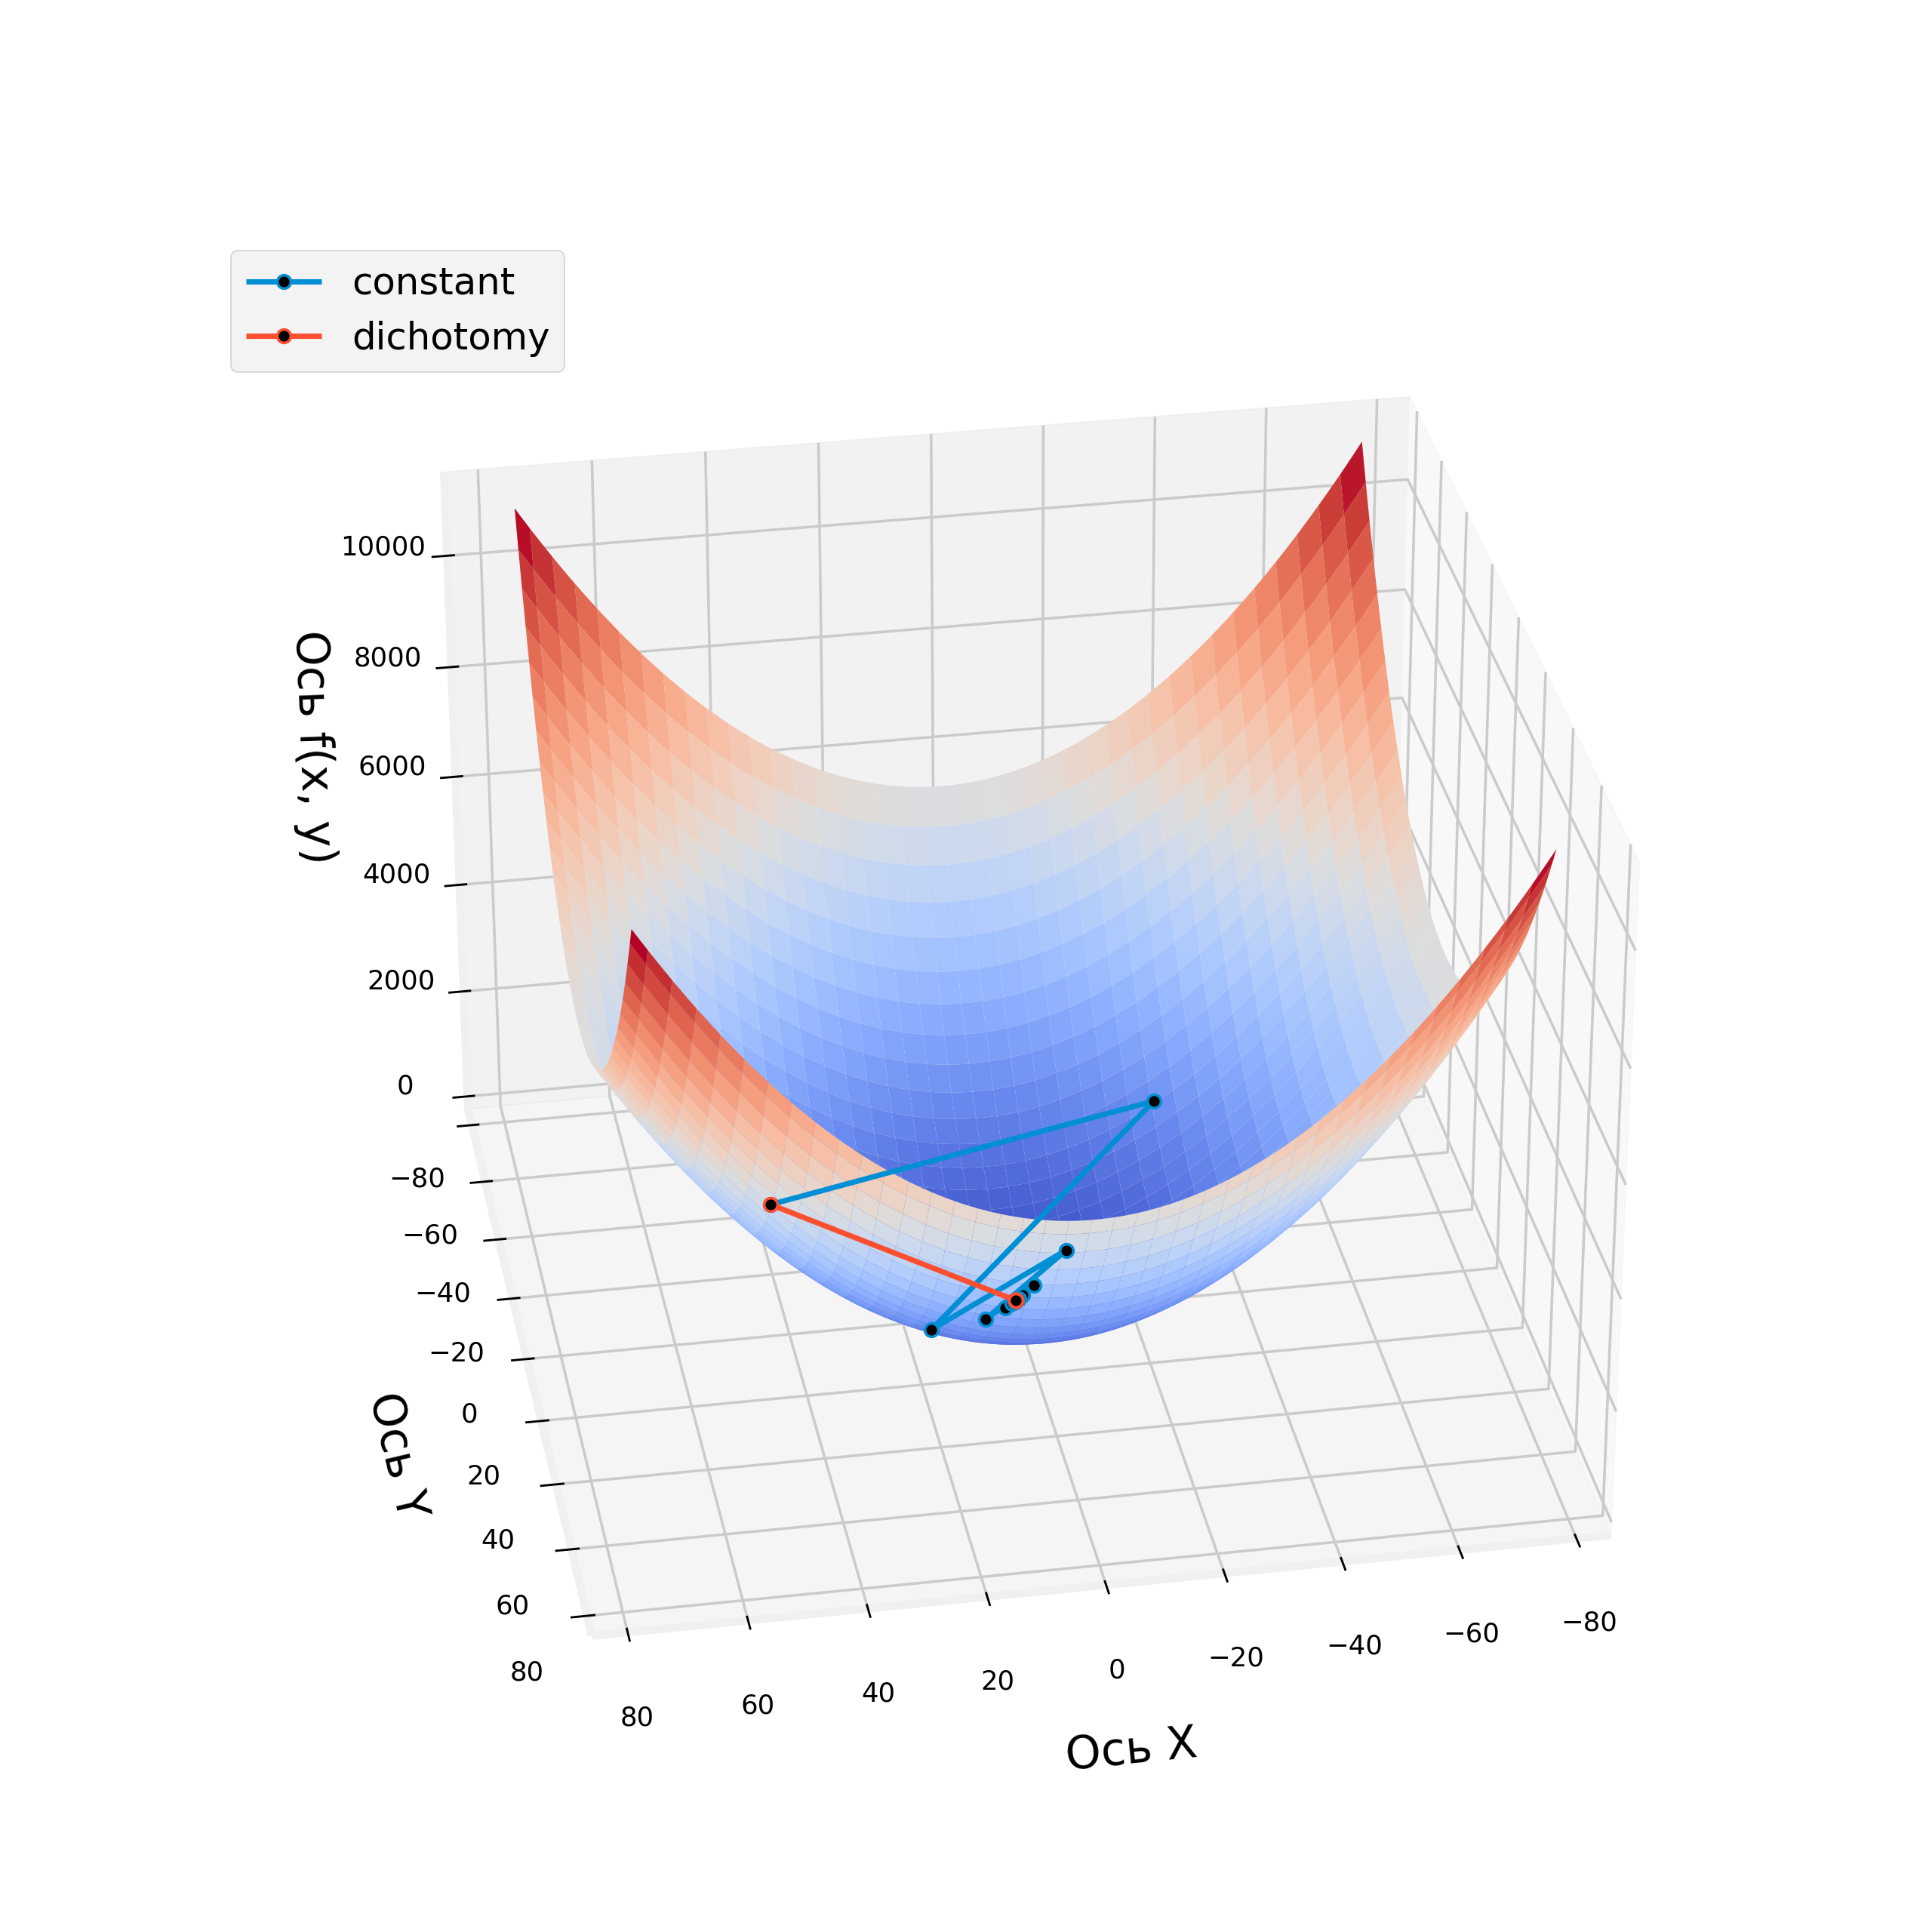
\includegraphics[scale=0.68]{Image/T4_E_F1_full_grad_constant_dichotomy.png}
			\caption*{\texttt{T4\_E\_F1\_full\_grad\_constant\_dichotomy}}
		\end{figure}
		\begin{figure}[H]
			\centering
			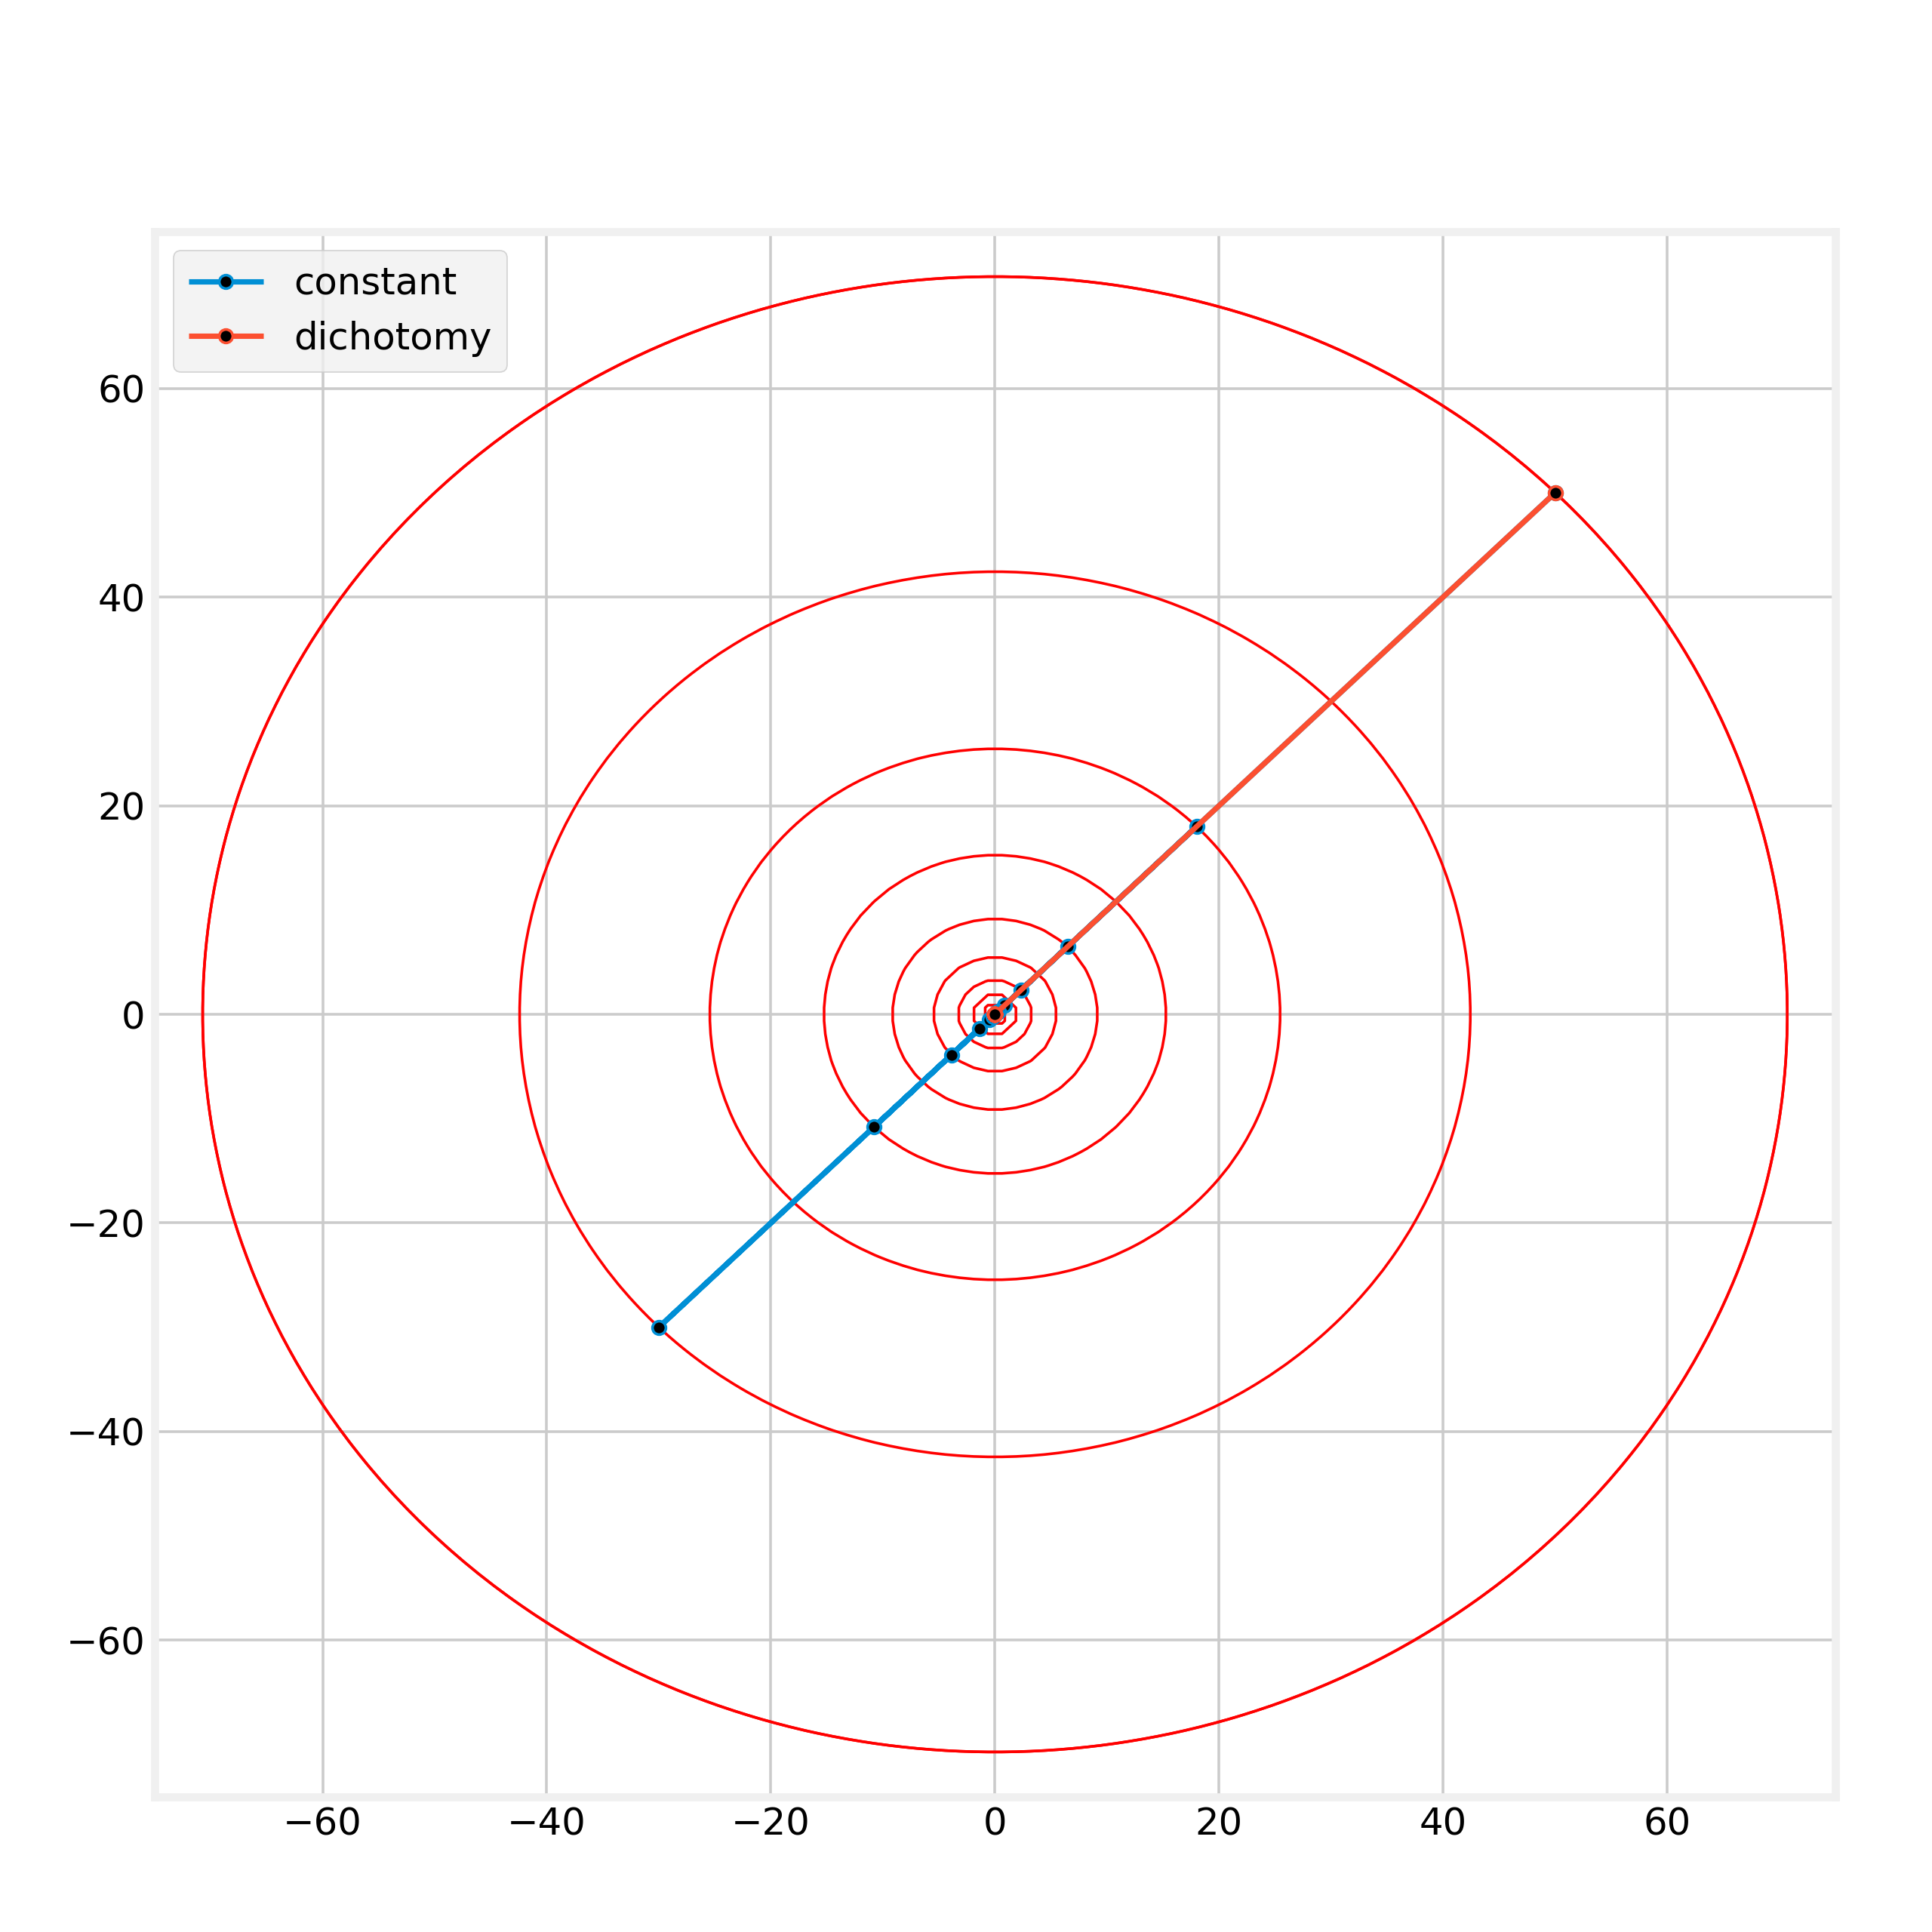
\includegraphics[scale=0.68]{Image/T4_E_F1_lines_grad_constant_dichotomy.png}
			\caption*{\texttt{T4\_E\_F1\_lines\_grad\_constant\_dichotomy}}
		\end{figure}
	\end{center}
	\begin{center}
		\begin{figure}[H]
			\centering
			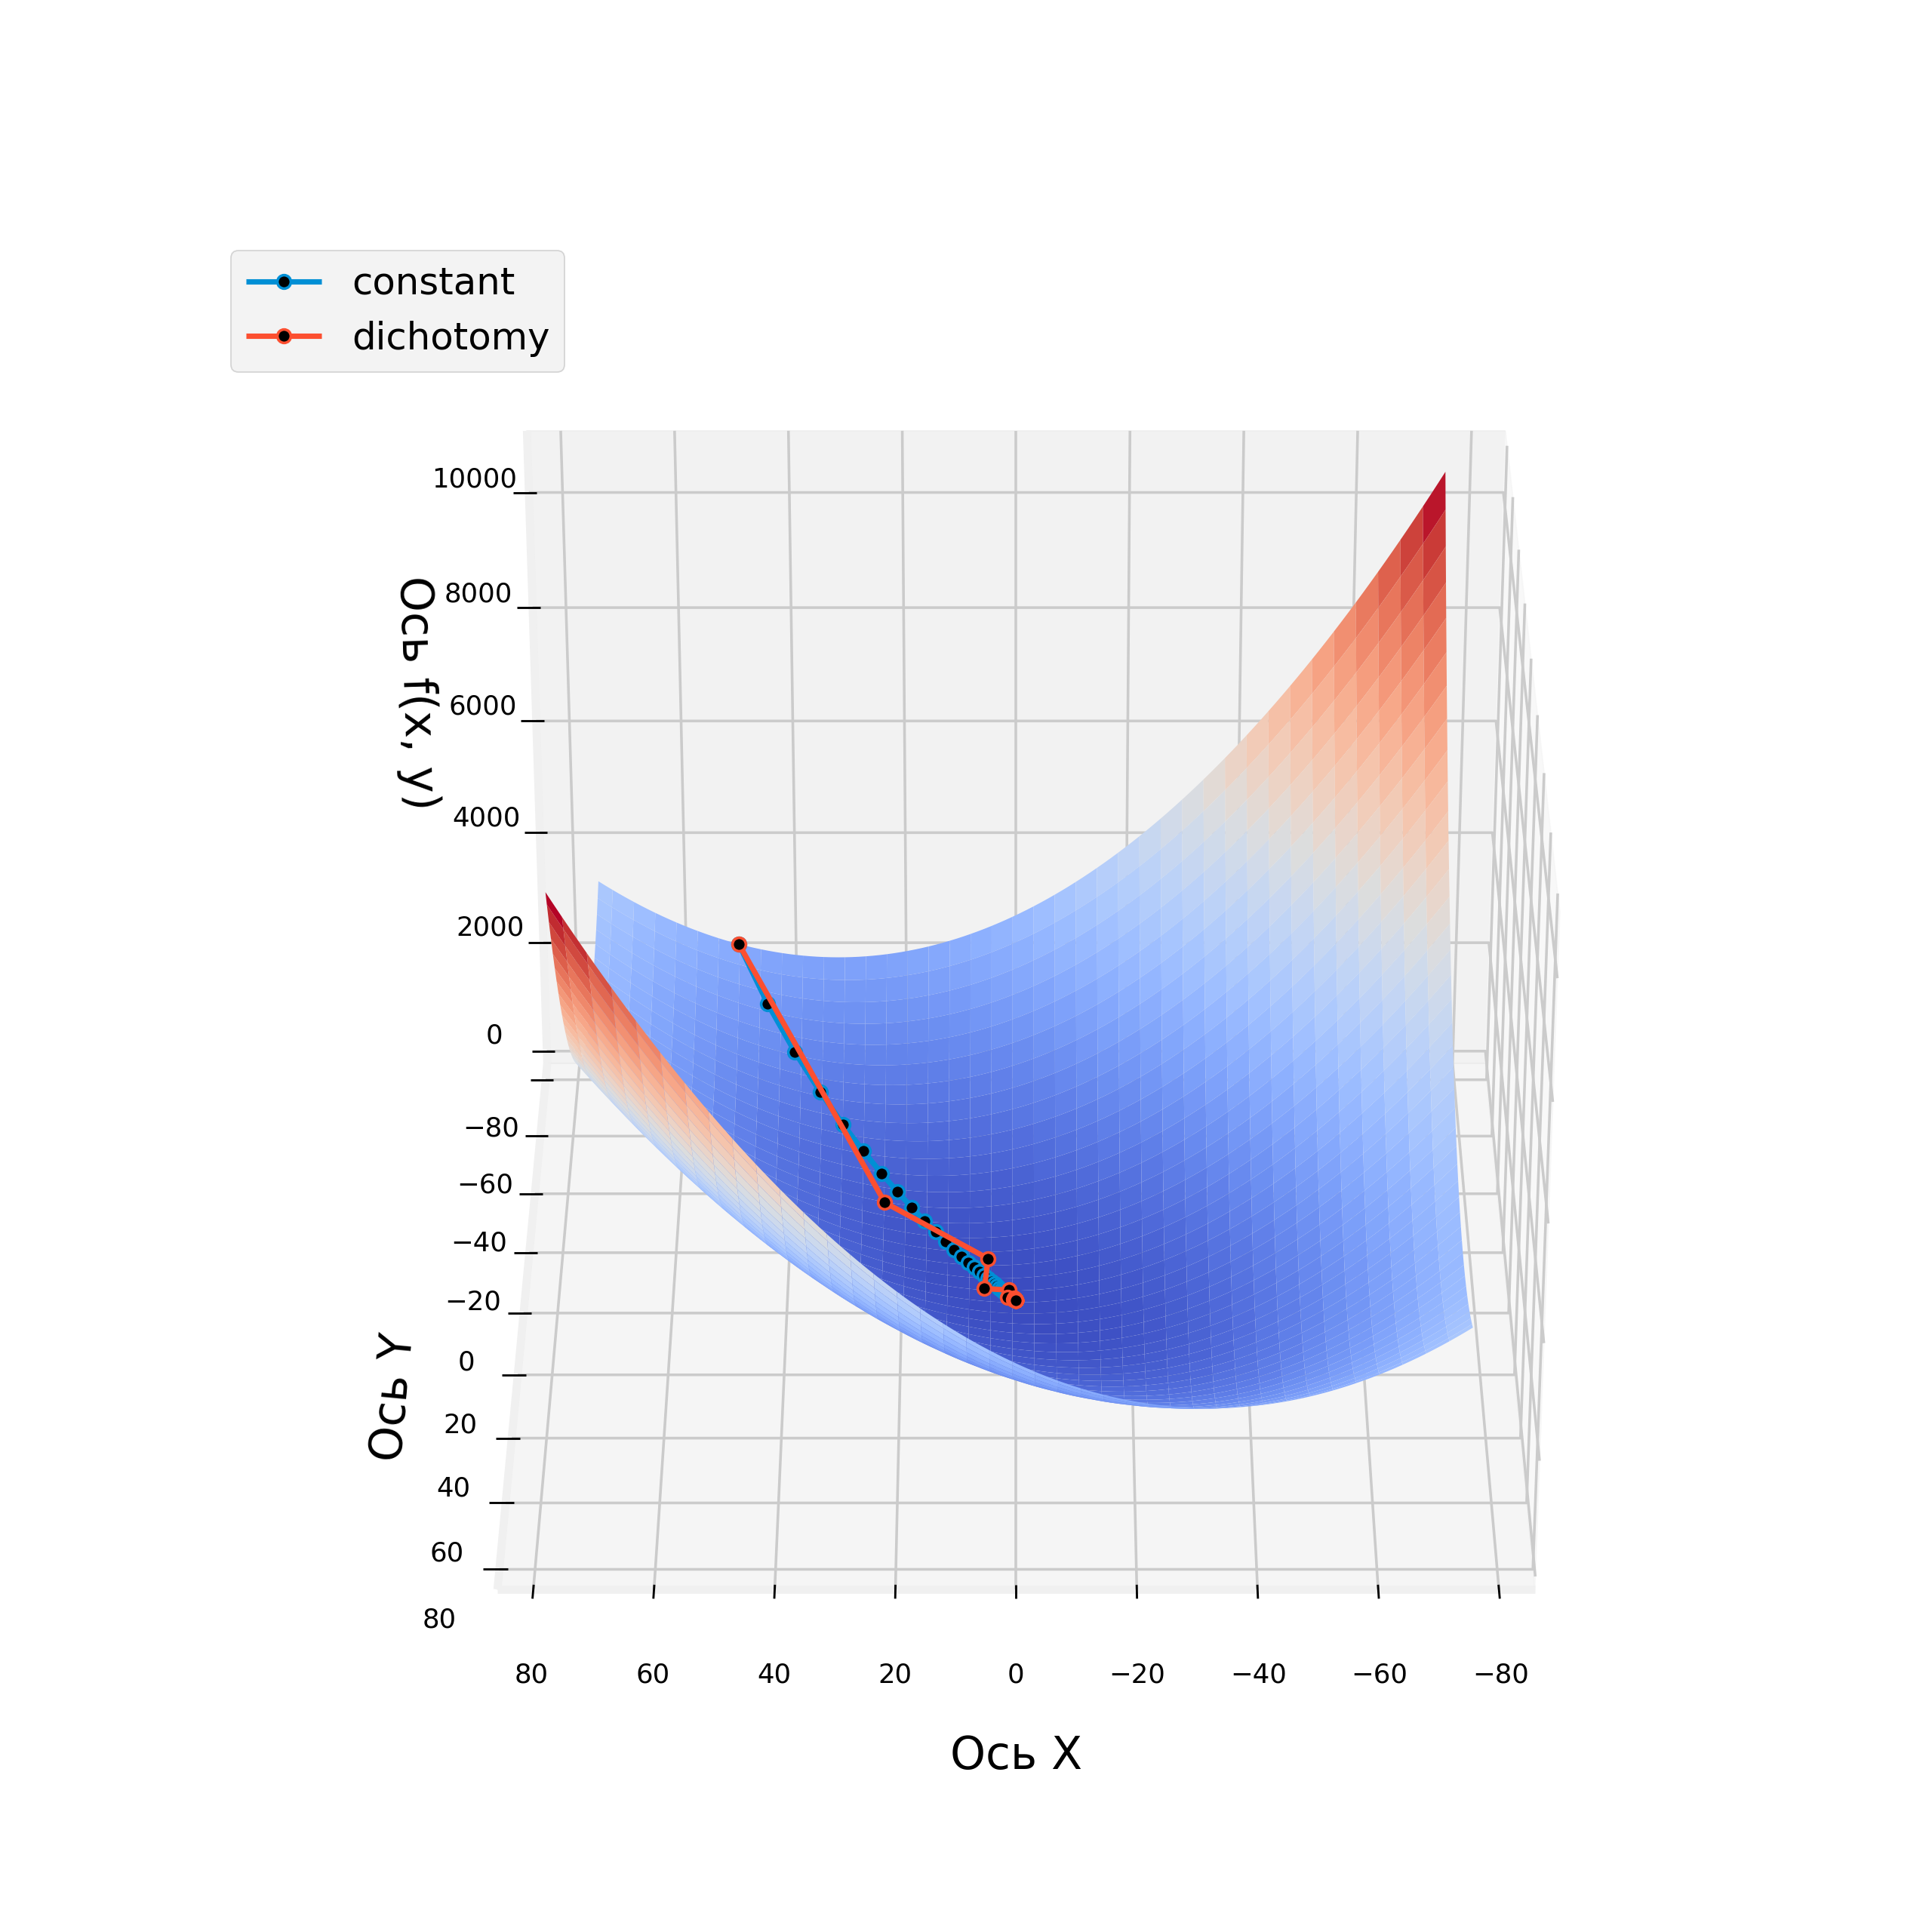
\includegraphics[scale=0.68]{Image/T4_E_F2_full_grad_constant_dichotomy.png}
			\caption*{\texttt{T4\_E\_F2\_full\_grad\_constant\_dichotomy}}
		\end{figure}
		\begin{figure}[H]
			\centering
			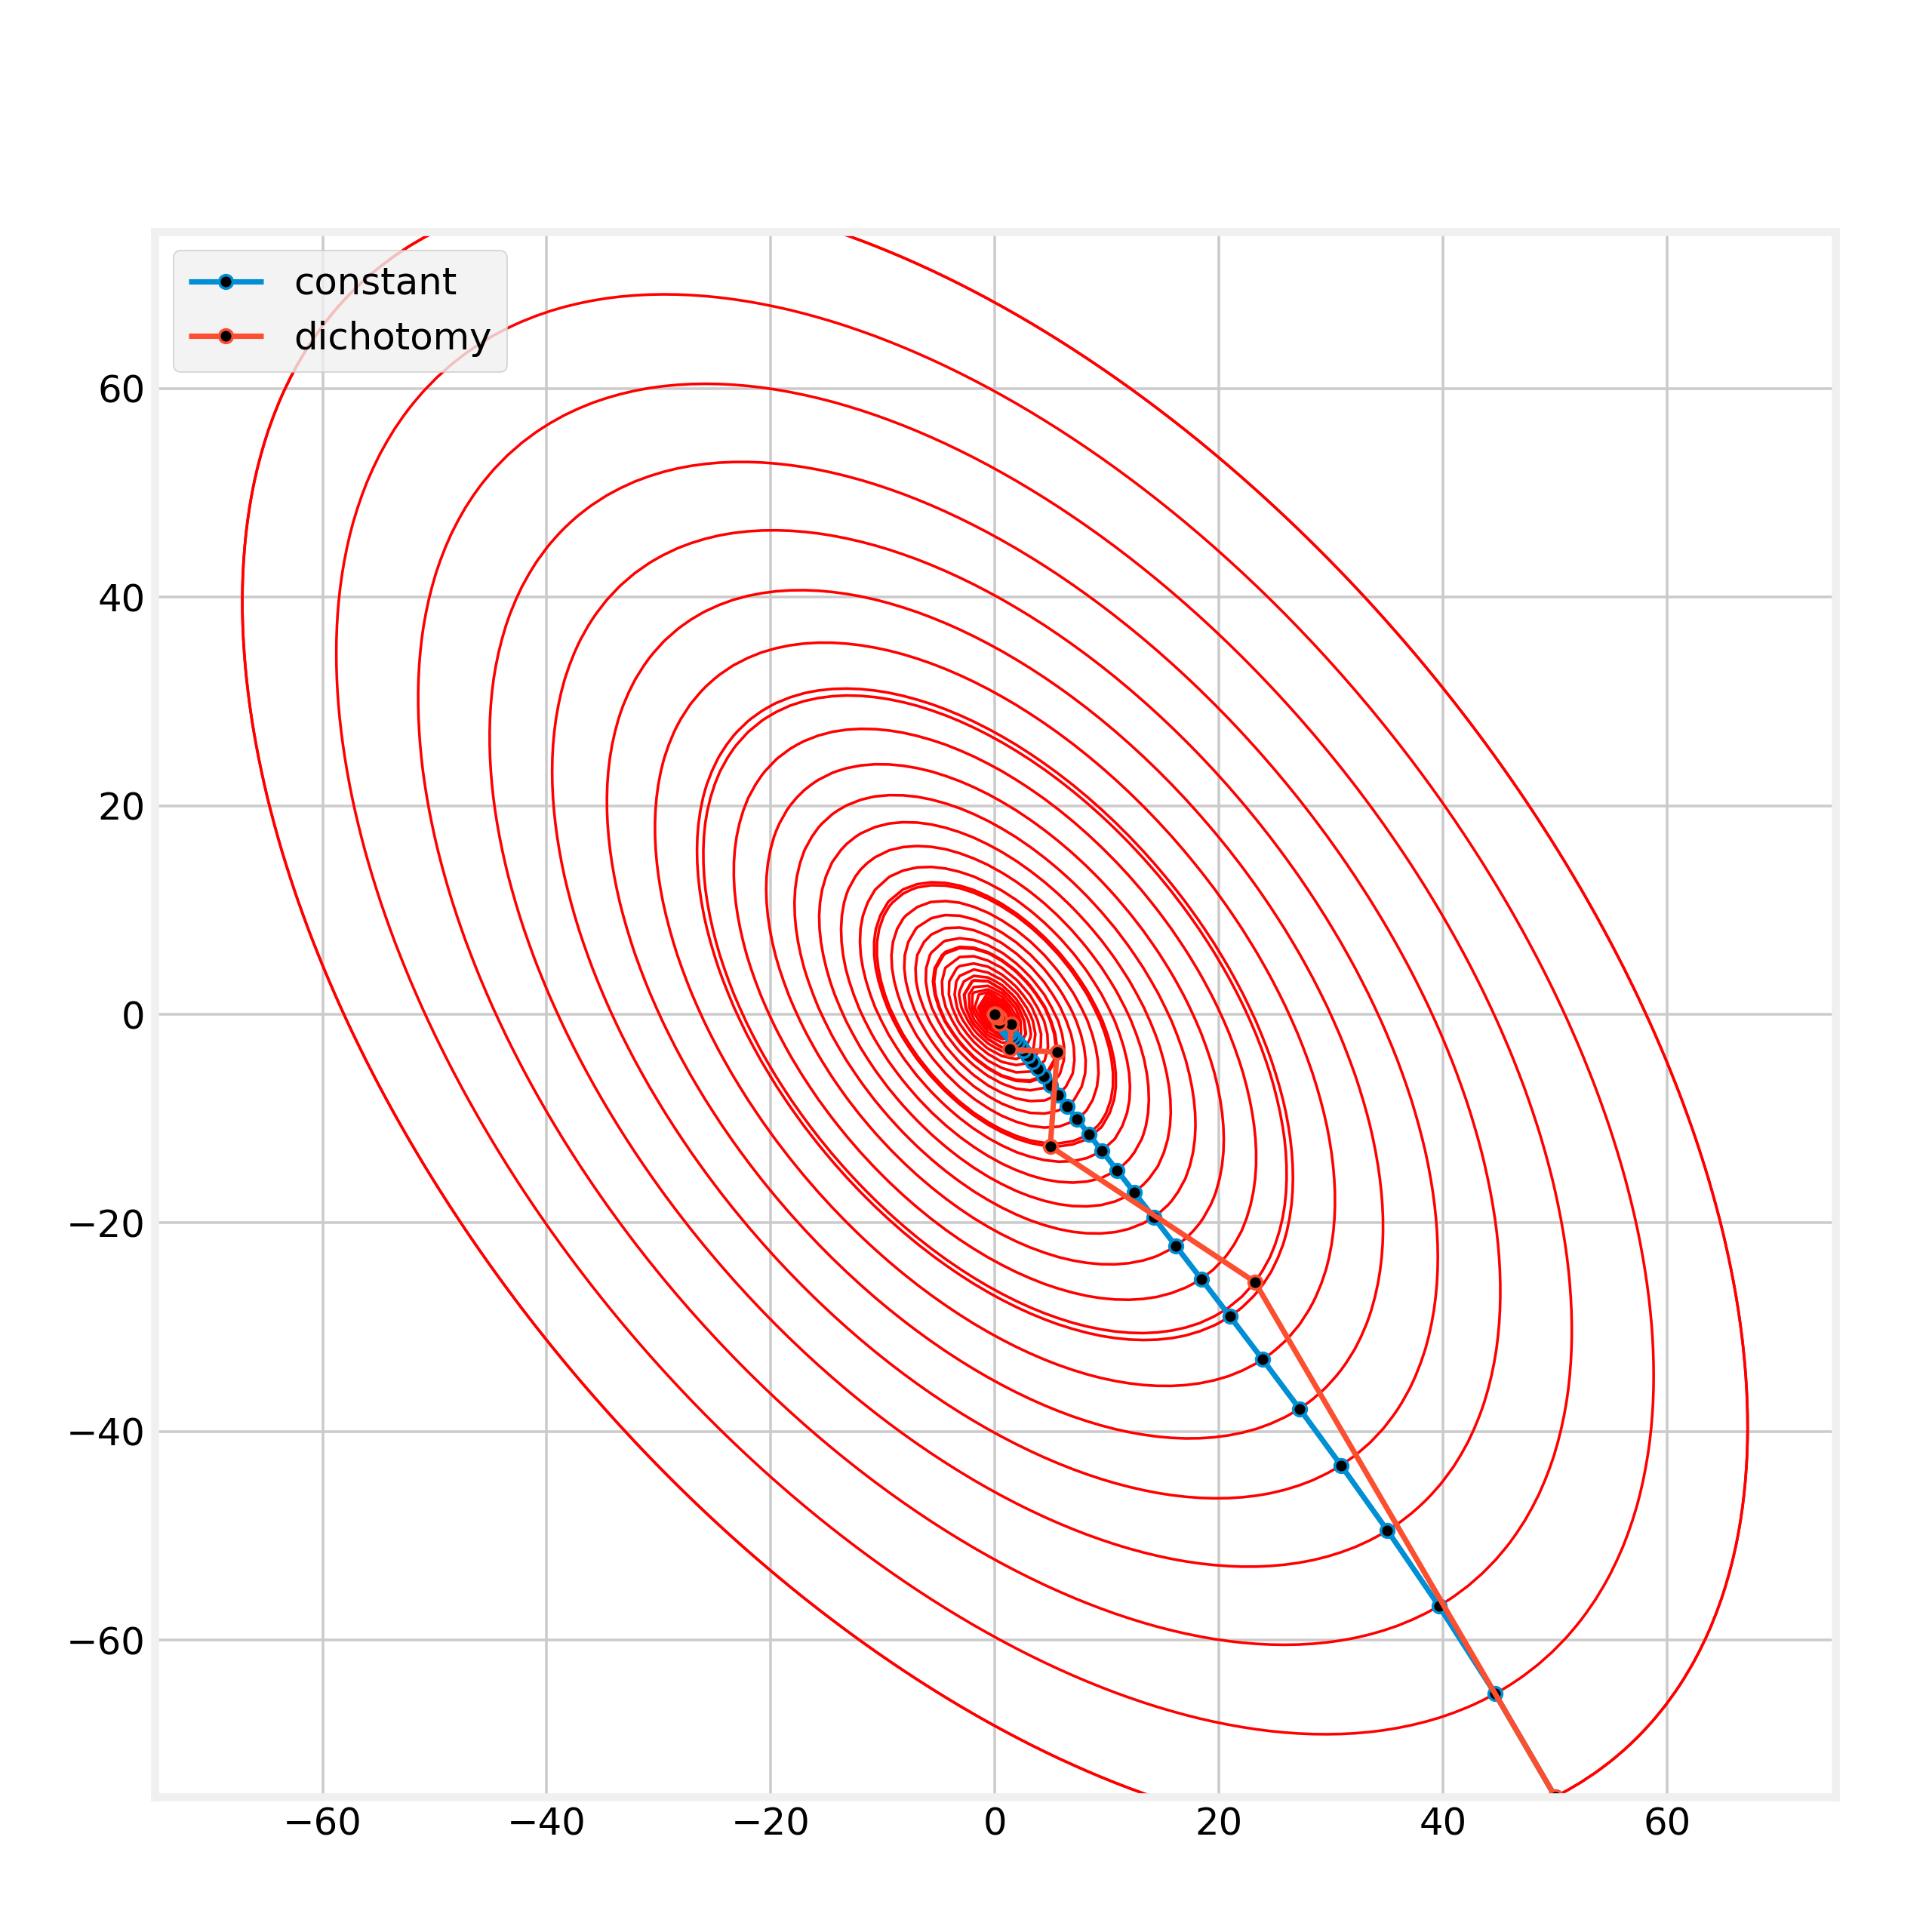
\includegraphics[scale=0.68]{Image/T4_E_F2_lines_grad_constant_dichotomy.png}
			\caption*{\texttt{T4\_E\_F2\_lines\_grad\_constant\_dichotomy}}
		\end{figure}
	\end{center}
	\newpage
	\section*{Задача 5}
	\subsection*{Постановка задачи}
	Реализуйте генератор случайных квадратичных функций $n$ переменных с числом обусловленности $k$.
	\subsection*{Решение}
	Для начала поймем, что такое \textit{число обусловленности}. По своей сущности, это нечто, что может показать насколько измениться значение функции при небольшом изменении аргумента. Для нахождения такого числа и, в следствии, нахождения вектора чисел, которые будут являться коэффициентами квадратичной сгенерированной функции. Для решении такой задачи мы могли воспользоваться правильными методами такими как \textit{теорема о сингулярном разложении}: возьмем некоторую матрицу $A$, возьмем его после разложении образовавшийся диагональную матрицу, тогда его (матрицы $A$) число обусловленности будет равно отношению максимального по модулю и минимального по модулю собственных чисел выбранной матрицы. Проблемой столь мощного инструментария заключается в том, что генерация подобной матрицы наивным методом может занимать немереное время, ибо асимптотику спектрального разложения, которое и является основным в сингулярном, никто предугадать не может.

	Тогда приходит идея менее безболезненная, но более радикальная: скажем, что наша матрица изначально была подана диагональной, а значит наша генерации функции сводится к вычислению $n$-чисел на диагонали матрицы.

	Итак, пусть дано число обусловленности $k$, положим $\text{MAX} = k \cdot \text{MIN}$~-- максимальное по модулю значение собственного числа матрицы, а в качестве минимального возьмем случайное число из ограниченного операционной системой диапазоном, например $[0, 2^{\log_{2}{X}} - 1]$. Тогда, наконец, все остальные элементы следует брать из диапазона $[\text{MIN} + 1, \text{MIN} \cdot k)$.

	В качестве промежуточного итога предоставим псевдо-алгоритм для решения этой задачи:
	\begin{lstlisting}
	function $random(l, r)$:
		return $randomized$ $\mathtt{Ret} \in [l, \ldots, r)$
	
	function $generate(n, k)$:
		$\text{MIN} \gets \text{random}(0, 2^{64} - 1)$
		$\text{MAX} \gets \text{MIN} \cdot k$
		$q \gets [\text{MIN},~\text{MAX},~x_{0}~\ldots,~x_{n - 3}], ~ \forall x_{i} = 0$

		$\forall i \in [2, n]$:
			$q_{i} \gets random(\text{MIN} + 1,~\text{MAX})$

		return q
	\end{lstlisting}
	\newpage
	\section*{Задача 6 и 7}
	\subsection*{Постановка задачи}
	Исследуйте зависимость числа итераций $T(n, k)$, необходимых градиентному спуску для сходимости в зависимости от размерности пространства $2 \leqslant n \leqslant 10^{3}$ и числа обусловленности оптимизируемой функции $1 \leqslant k \leqslant 10^{3}$. 
	\subsection*{Решение}
	Для понимания числа итераций, необходимых градиентному спуску для сходимости в некоторый приближенный минимум от двух меняющихся переменных $n$ и $k$ мы, для ускорения и недопущения плохо сгенерированных функций, поставим два условия остановки цикла: первое~-- это самая простая проверка критерия на $\varepsilon$, запрашивая тем самым, если ли дальше смысл идти, второе~-- это предельное количество итераций, если нынешнее число все же превысило предел, то цикл тут же останавливается.

	В качестве промежуточного итога предоставим псевдо-алгоритм для решения этой задачи:
	\begin{lstlisting}
		function $\nabla{f(x)}$:
			return $\left[f(x)\dfrac{\partial}{\partial{x^{0}}}, ~ f(x)\dfrac{\partial}{\partial{x^{1}}}, ~ \ldots, ~ f(x)\dfrac{\partial}{\partial{x^{n - 1}}}\right]$
		
		function $scale(p_1, ~ p_2)$:
			$l, r \gets 0, 1$

			$\forall~\infty$:
				$m \gets \dfrac{l + r}{2}$
				$\alpha \gets \lambda \cdot (m \pm \varepsilon)$
				$a, b \gets p_1 - p_2 \cdot \alpha$
		
				if $a < b$ then
					$l \gets m$
				else
					$r \gets m$
		
				if $|l - r| \leqslant \varepsilon$ then
					break
		
		function $gradient\_dichotomy$:
			$x_{0} \gets \text{INIT}$
			$\lambda \gets \texttt{const}$
			$\text{counter} \gets 0$

			$\forall~i \in [1, k]$:
				$x_{i} \gets x_{i - 1} - \lambda \cdot \texttt{scale}(f(x_{i - 1}), \nabla{f(x_{i - 1})})$

				if $|x_{i} - x_{i - 1}| \leqslant \varepsilon$ then
					break

				if $\text{counter} = \text{max\_iter}$ then
					break
				else
					$\text{counter}++$
		
			return $\text{counter}$
		
		function $random(l, r)$:
			return $randomized$ $\mathtt{Ret} \in [l, \ldots, r)$
		
		function $generate(n, k)$:
			$\text{MIN} \gets \text{random}(0, 2^{64} - 1)$
			$\text{MAX} \gets \text{MIN} \cdot k$
			$q \gets [\text{MIN},~\text{MAX},~x_{0}~\ldots,~x_{n - 3}], ~ \forall x_{i} = 0$
		
			$\forall i \in [2, n]$:
				$q_{i} \gets random(\text{MIN} + 1,~\text{MAX})$
		
			return q
		
		function $main$:
			$q \gets \{\}$

			$\forall n \in [2, 10^{3}]$ do
				$\forall k \in [1, 10^{3}]$ do
					$q \cup \text{gradient(generate(n, k))}$
	\end{lstlisting}
	\subsection*{Исследовательская часть}
	Интерпретируем наш псевдо-алгоритм в жизнь и выведем графики зависимости $n$, $k$ от количества итераций до сходимости. В качестве критериев мы поставим уже знакомые нам условия остановки: предельное число и сходимости от минимальной точки на расстоянии $\varepsilon$. Рассмотрим с шагом $0.01$, для всех $k \in [1, 1000]$ при $n = 2$
	\begin{figure}[H]
		\centering
	 	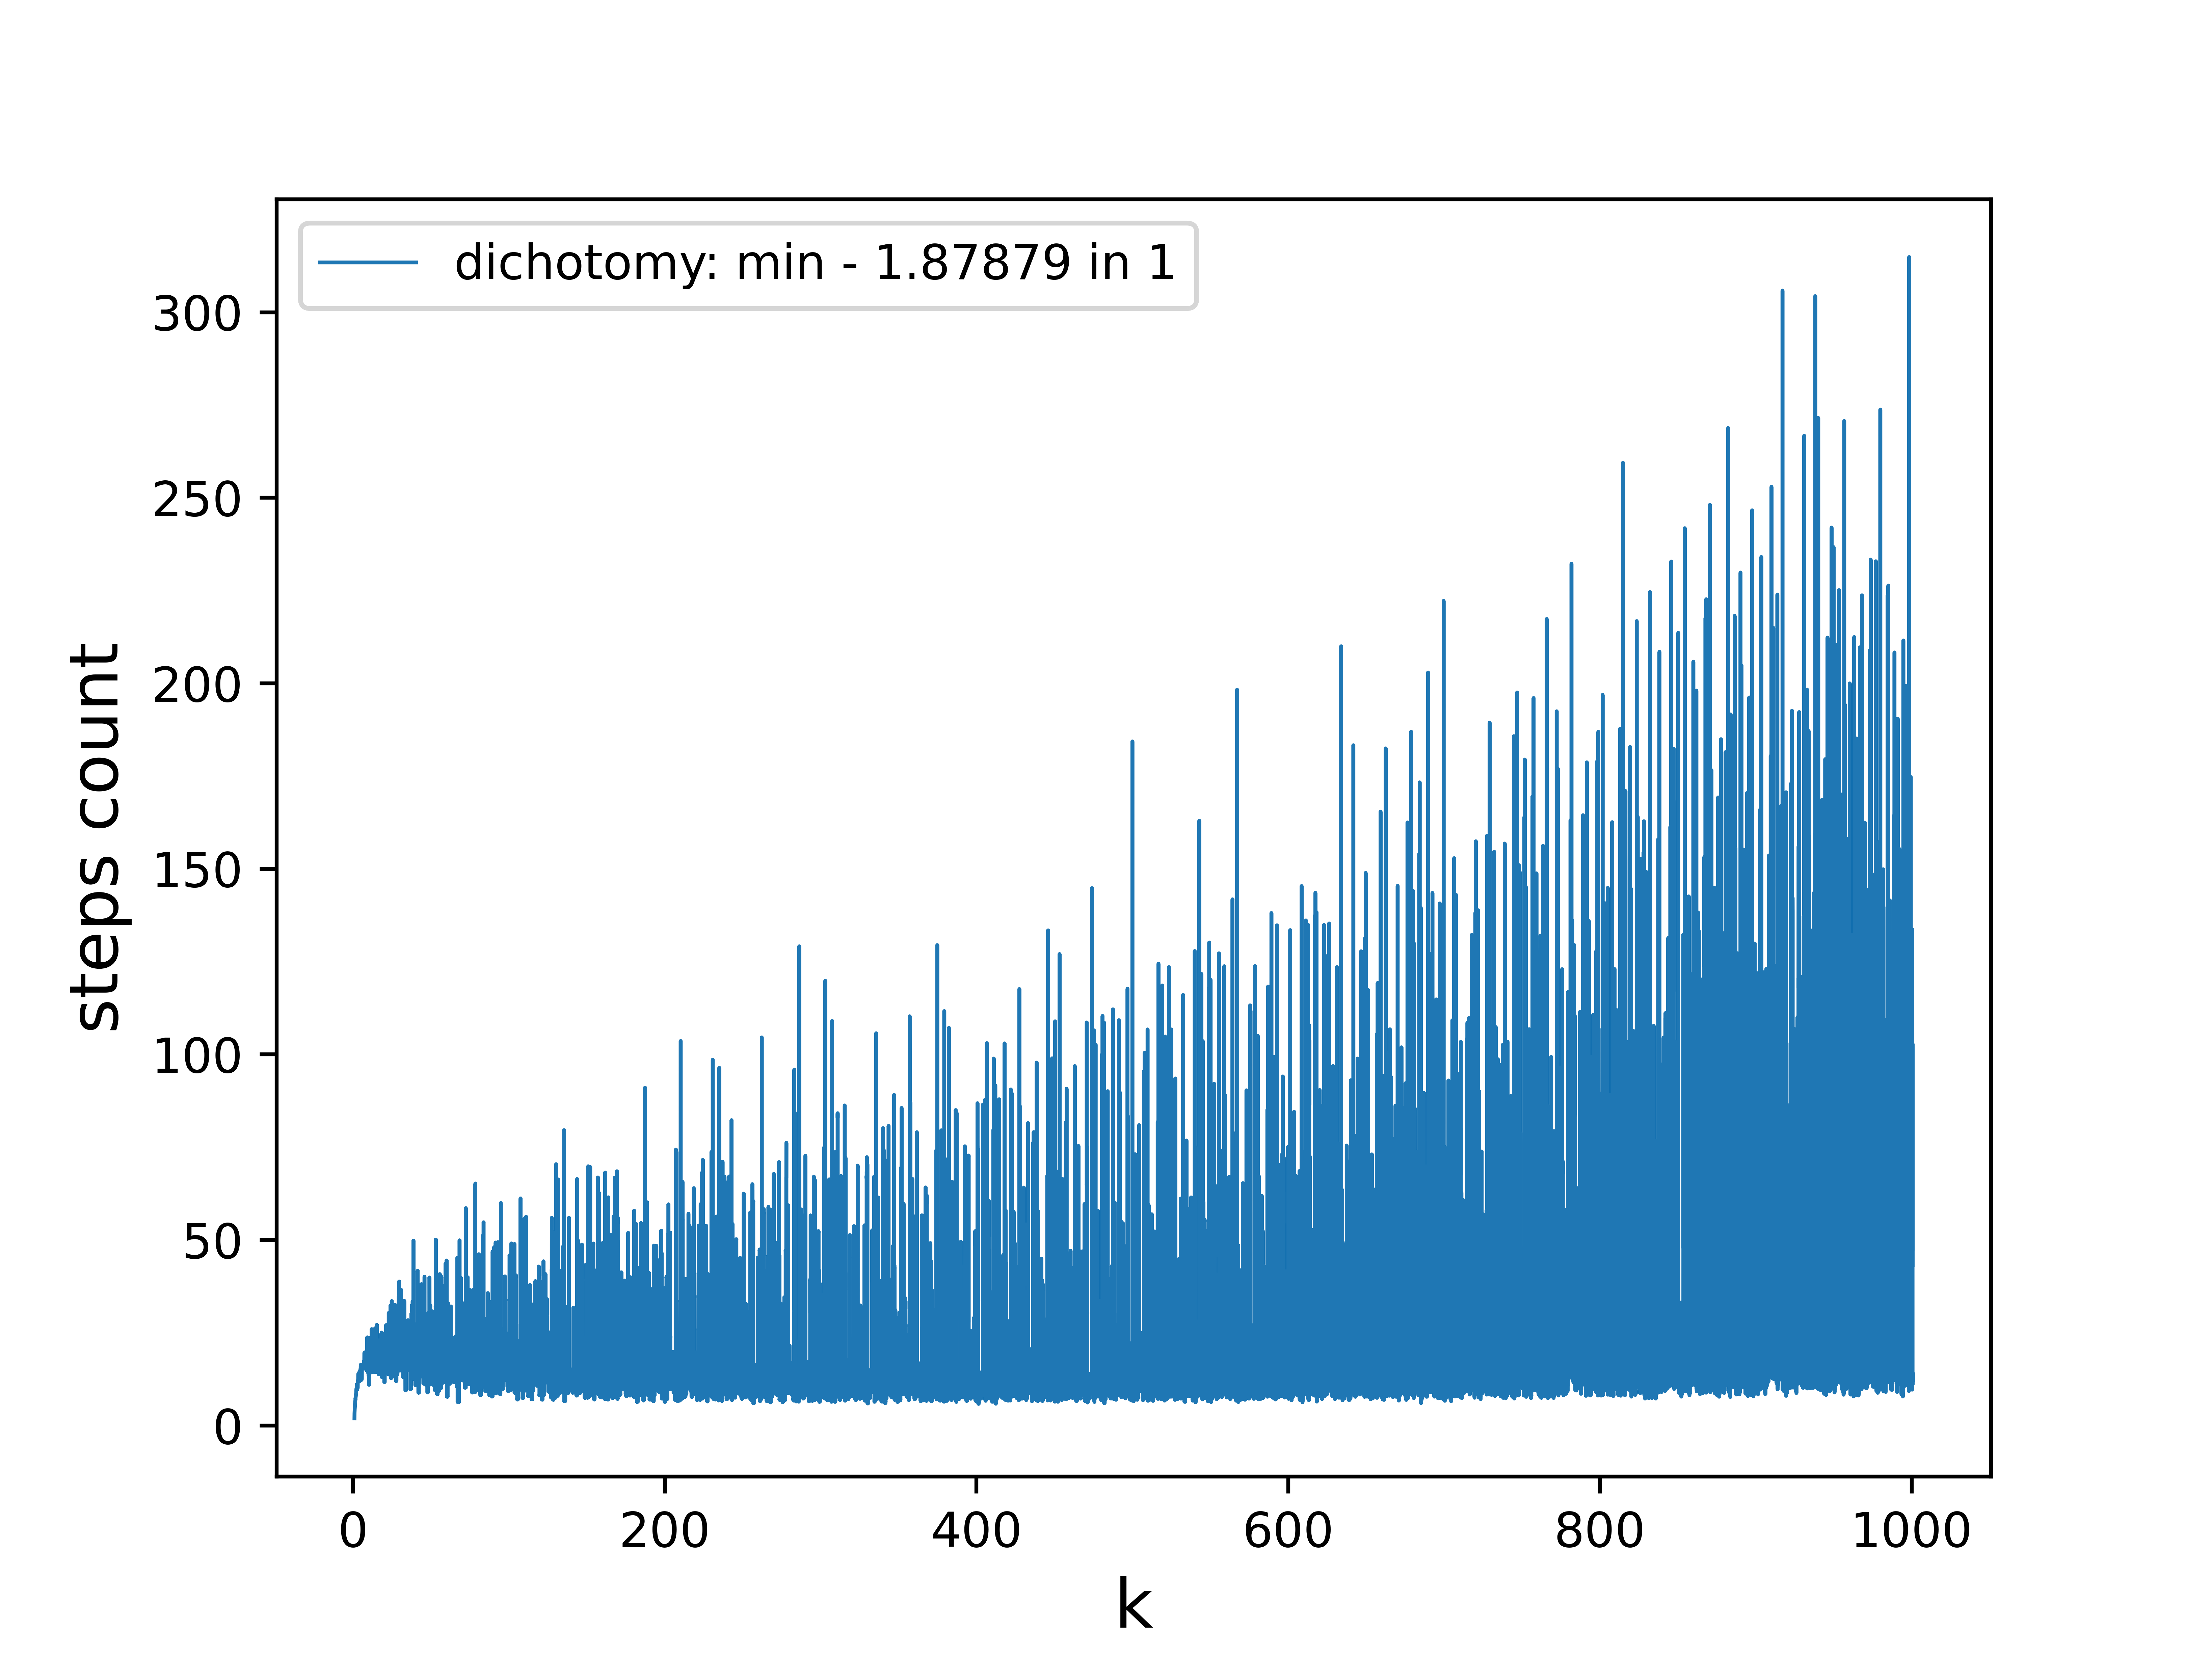
\includegraphics[scale=0.78]{HQ/T6_2D_k_dichotomy_n2_1_1000_n2_step_0_01.png}
		\caption*{\texttt{T6\_2D\_k\_dichotomy\_n2\_1\_1000\_n2\_step\_0\_01}}
	\end{figure}
	Заметим, что у нас появляются выбросы при некоторых больших значениях $k$. Число шагов также, заметим, почти линейно возрастает с увеличением $k$.

	Теперь рассмотрим случай с $k = 50$ при всех $n \in [2, 1000]$.
	\begin{figure}[H]
		\centering
		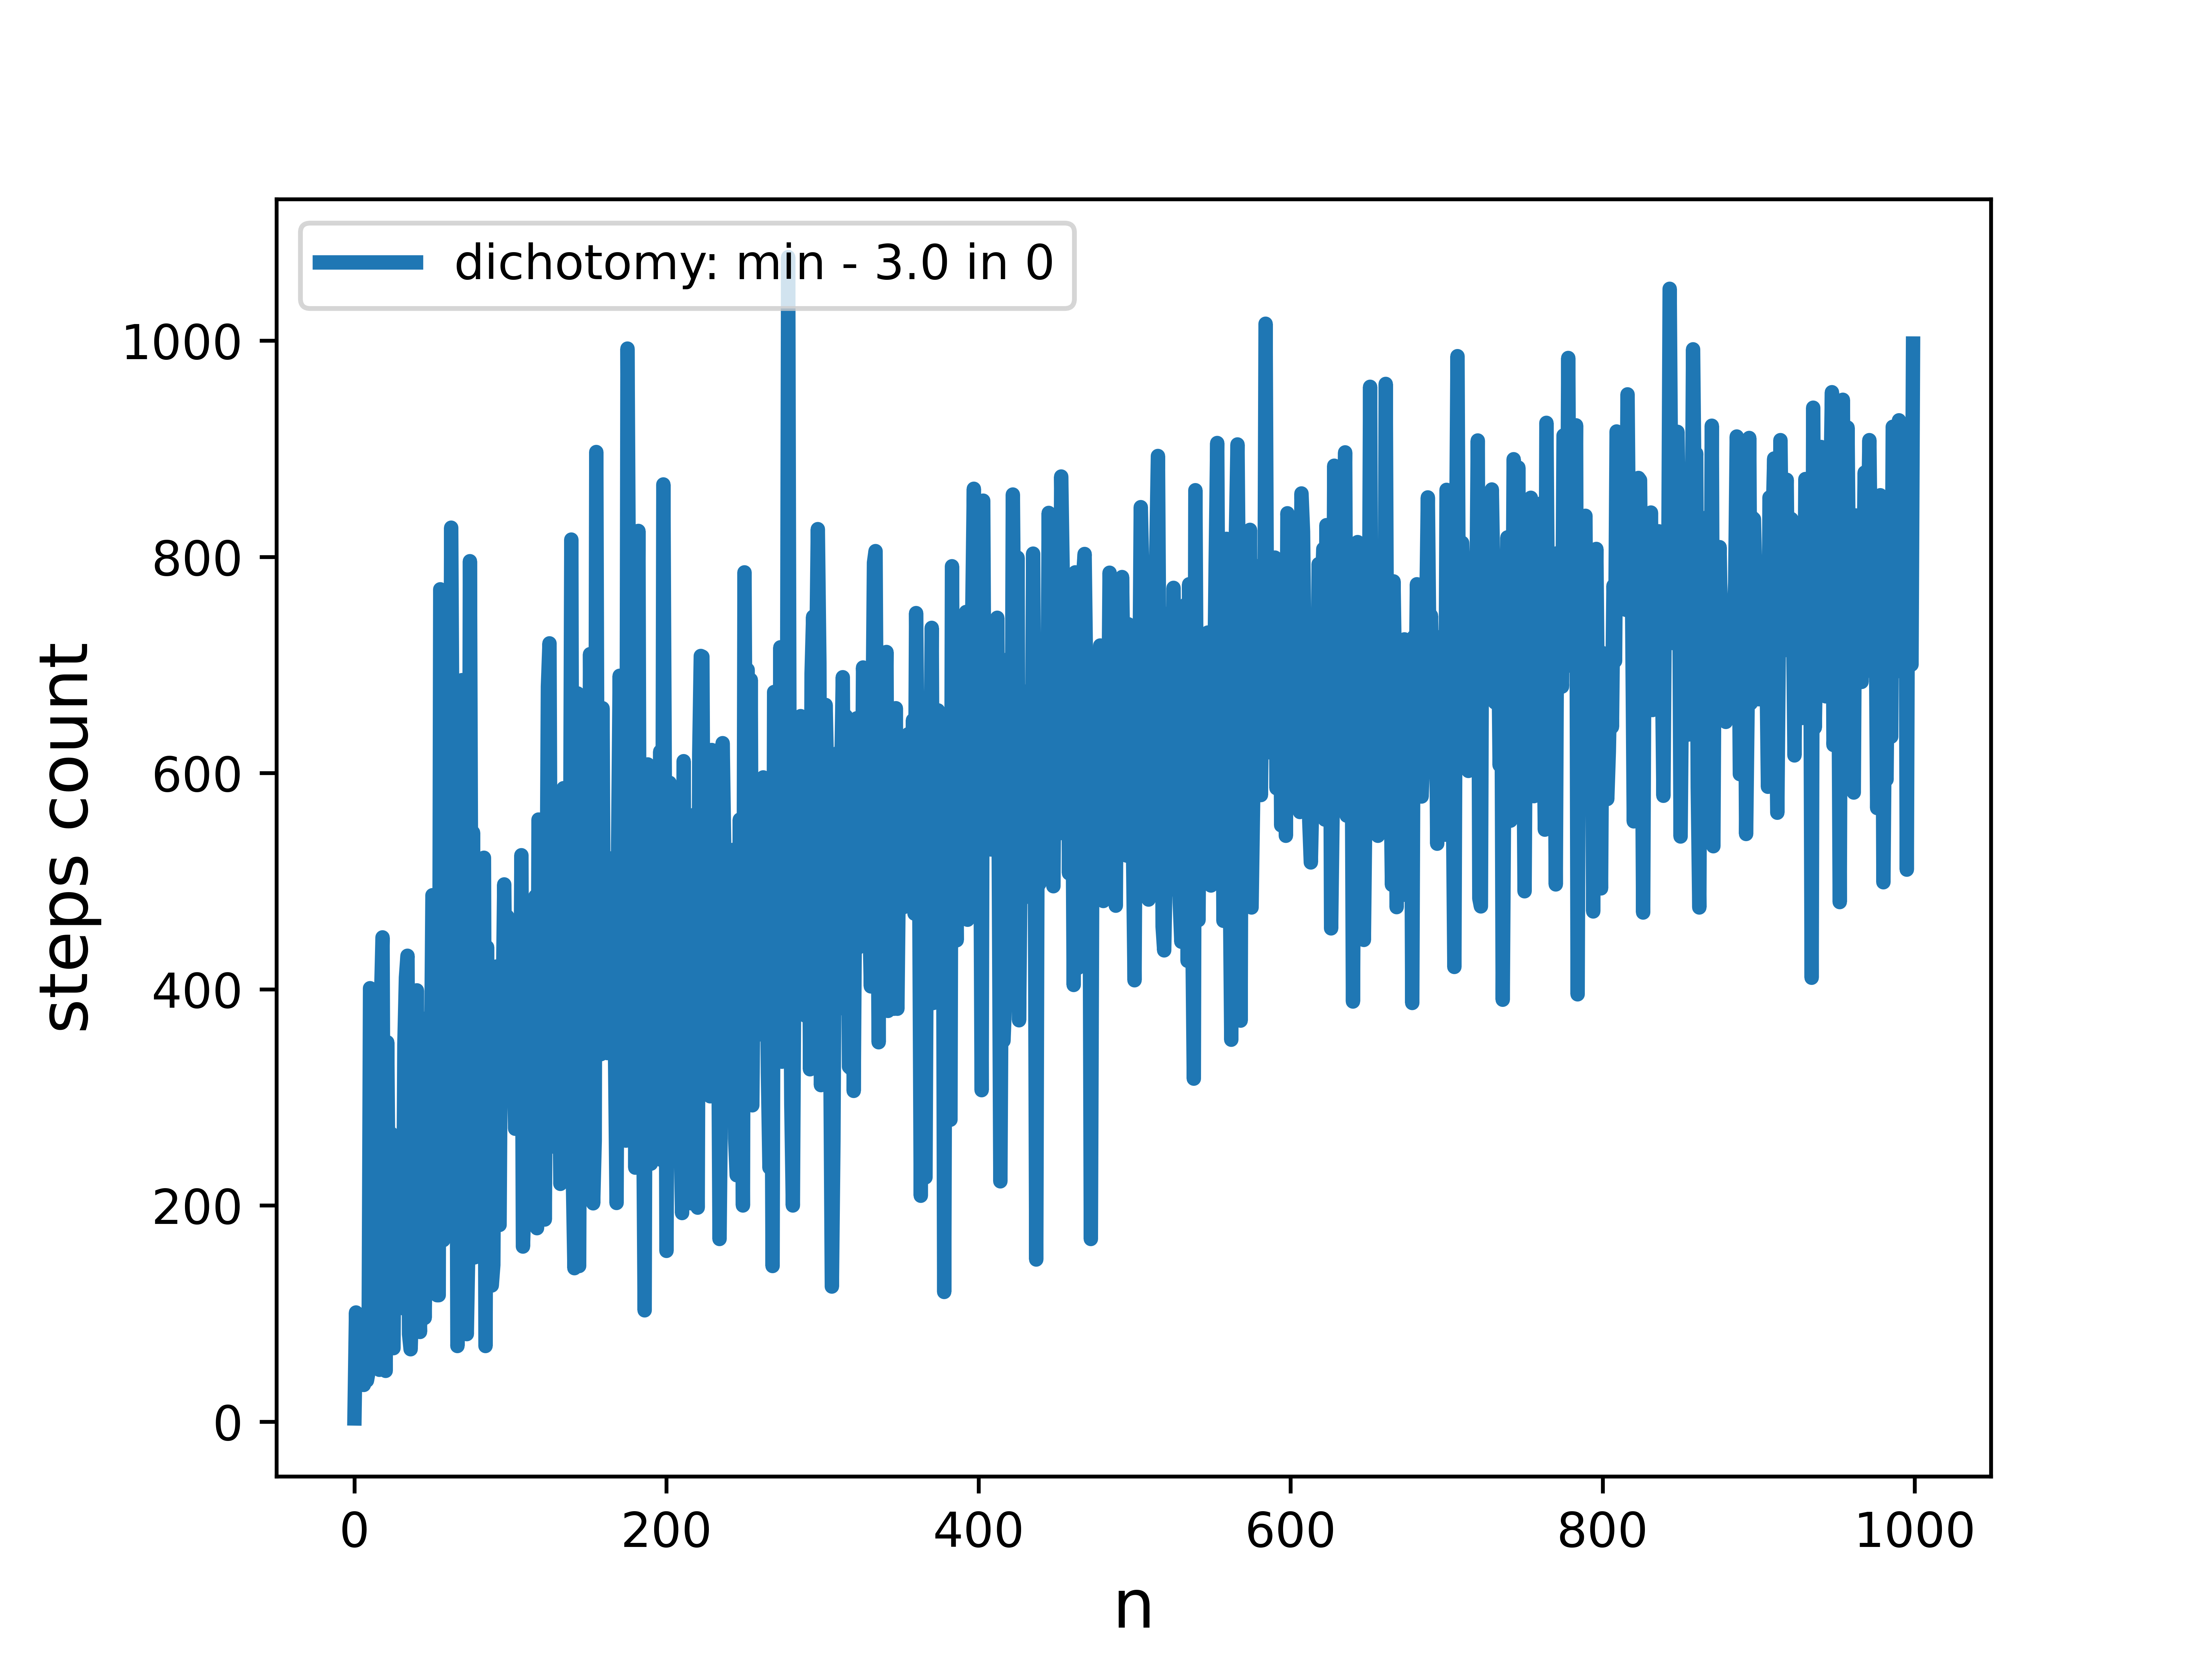
\includegraphics[scale=0.78]{HQ/T6_2D_n_dichotomy_k50.png}
		\caption*{\texttt{T6\_2D\_n\_dichotomy\_k50}}
	\end{figure}
	Здесь мы получаем более честную зависимости числа шагов от $n$ при фиксированном $k$, так как для некоторого $n'$ усредненно получается одно и то же число шагов.
	\newpage
	\section*{Дополнительное задание}
	\subsection*{Постановка задачи}
	Реализуйте одномерный поиск с учетом условий Вольфе и исследуйте его эффективность. Сравните полученные результаты с реализованными ранее методами.
	\subsection*{Решение}
	Вернемся к истокам, а именно к самой первой задаче. Там мы обсуждали и говорили о градиентном спуске как о методе более быстрого поиска приближенного минимального значения поиском аргумента $x$. Тогда мы сказали, что это все же неплохой инструментарий для совершенно простых функций. В последующих пунктах мы доказали это с помощью метода дихотомии, что иногда нам нужно уменьшать шаг, чтобы дойти до этого самого минимума, так как с постоянным шагом есть ненулевая вероятность навсегда оказаться в вечных скитаниях поиска при перепрыгивании бездны.

	Задача поиском с \textit{учетом условий Вольфе} помогает нам избавиться от ограничения изменять шаг, только уменьшая его, мы можем его и увеличивать. Положим, что $\nabla{f^{T}_{k}p_{k}} < 0$, тогда возьмем изначальный вариант вида $x_{k + 1} = x_{k} + \alpha \cdot p_{k}$ и скажем, что $\alpha$ удовлетворяет условиям Вольфе, если:
	\begin{itemize}
		\item $f(x_{k} + \alpha \cdot p_{k}) \leqslant f(x_{k}) + c_{1} \cdot \alpha \cdot \nabla{f^{T}_{k}p_{k}}$
		\item $\nabla{f(x_{k} + \alpha \cdot p_{k})^{T}p{k}} \geqslant c_{2} \cdot \nabla{f^{T}_{k}p_{k}}$
	\end{itemize}
	где в качестве $c_{1}$ выбирается, как правило, при окрестности нуля, то есть $c_{1} \approx 10^{-6}$, а $c_{2}$, наоборот, в окрестности единицы, например, $c_{2} = 0.9$. Разберемся с условиями: первое говорит о том, что если мы делаем какой-то большой $learning~rate$ при итерации, то и изменение значения по модулю должно быть достаточно большим; второе же~-- посчитанный градиент в той точке, куда мы собираемся пойти, должен быть в несколько раз больше, чем текущий.

	На основе этих данных мы можем задать что-то подобие на бинарный поиск по ответу, где в случае если наша точка не удовлетворена первым условие, то мы сдвигаем как бы правую границу, в случае неудовлетворенности второй~-- левую. Наконец, в если оба удовлетворены~-- возвращаем значение. В качестве промежуточного итога предоставим псевдо-алгоритм для решения этой задачи:
	\begin{lstlisting}
		function $f(x)$:
			/*$implementation~defined$*/
		
		function $\nabla{f(x)}$:
			return $\left[f(x)\dfrac{\partial}{\partial{x^{0}}}, ~ f(x)\dfrac{\partial}{\partial{x^{1}}}, ~ \ldots, ~ f(x)\dfrac{\partial}{\partial{x^{n - 1}}}\right]$

		function $first(\alpha)$:
			$l \gets f(x_{k} + \alpha \cdot p_{k})$
			$r \gets f(x_{k}) + c_{1} \cdot \alpha \cdot \nabla{f^{T}_{k}p_{k}}$
			return $l \leqslant r$

		function $second(\alpha)$:
			$l \gets \nabla{f(x_{k} + \alpha \cdot p_{k})^{T}p{k}}$
			$r \gets c_{2} \cdot \nabla{f^{T}_{k}p_{k}}$
			return $l \geqslant r$

		function $find(\alpha)$:
			$\alpha_{\text{low}} \gets 0$
			$\alpha_{\text{high}} \gets \infty$
			$\alpha_{\text{prev}} \gets 0$
			$\alpha_{\text{current}} \gets \alpha$

			$\forall~\infty$:
				if not $first(\alpha)$ then
					$\alpha_{\text{high}} \gets \alpha_{\text{current}}$
					$\alpha_{\text{current}} \gets \dfrac{\alpha_{\text{low}} + \alpha_{\text{high}}}{2}$
				else if not $second(\alpha)$ then
					$\alpha_{\text{low}} \gets \alpha_{\text{current}}$
					if $\alpha_{\text{high}} \equiv \infty$:
						$\alpha_{\text{current}} \gets 2 \cdot \alpha_{\text{low}}$
					else
						$\alpha_{\text{current}} \gets \dfrac{\alpha_{\text{low}} + \alpha_{\text{high}}}{2}$
				else
					return $\alpha_{\text{current}}$

				if $\alpha_{\text{current}} - \alpha_{\text{prev}} \leqslant \varepsilon$:
					break

				$\alpha_{\text{prev}} \gets \alpha_{\text{current}}$

			return $\alpha_{\text{current}}$
	\end{lstlisting}
	\subsection*{Пример}
	В качестве примера мы рассмотрим простую функцию параболоида $f(x, y) = x^{2} + y^{2}$ и начнем мы искать приближенный минимум из точки $\langle-40, ~ 50\rangle$. Запустим алгоритм и посмотрим на выходные значения.
	\begin{figure}[H]
		\centering
		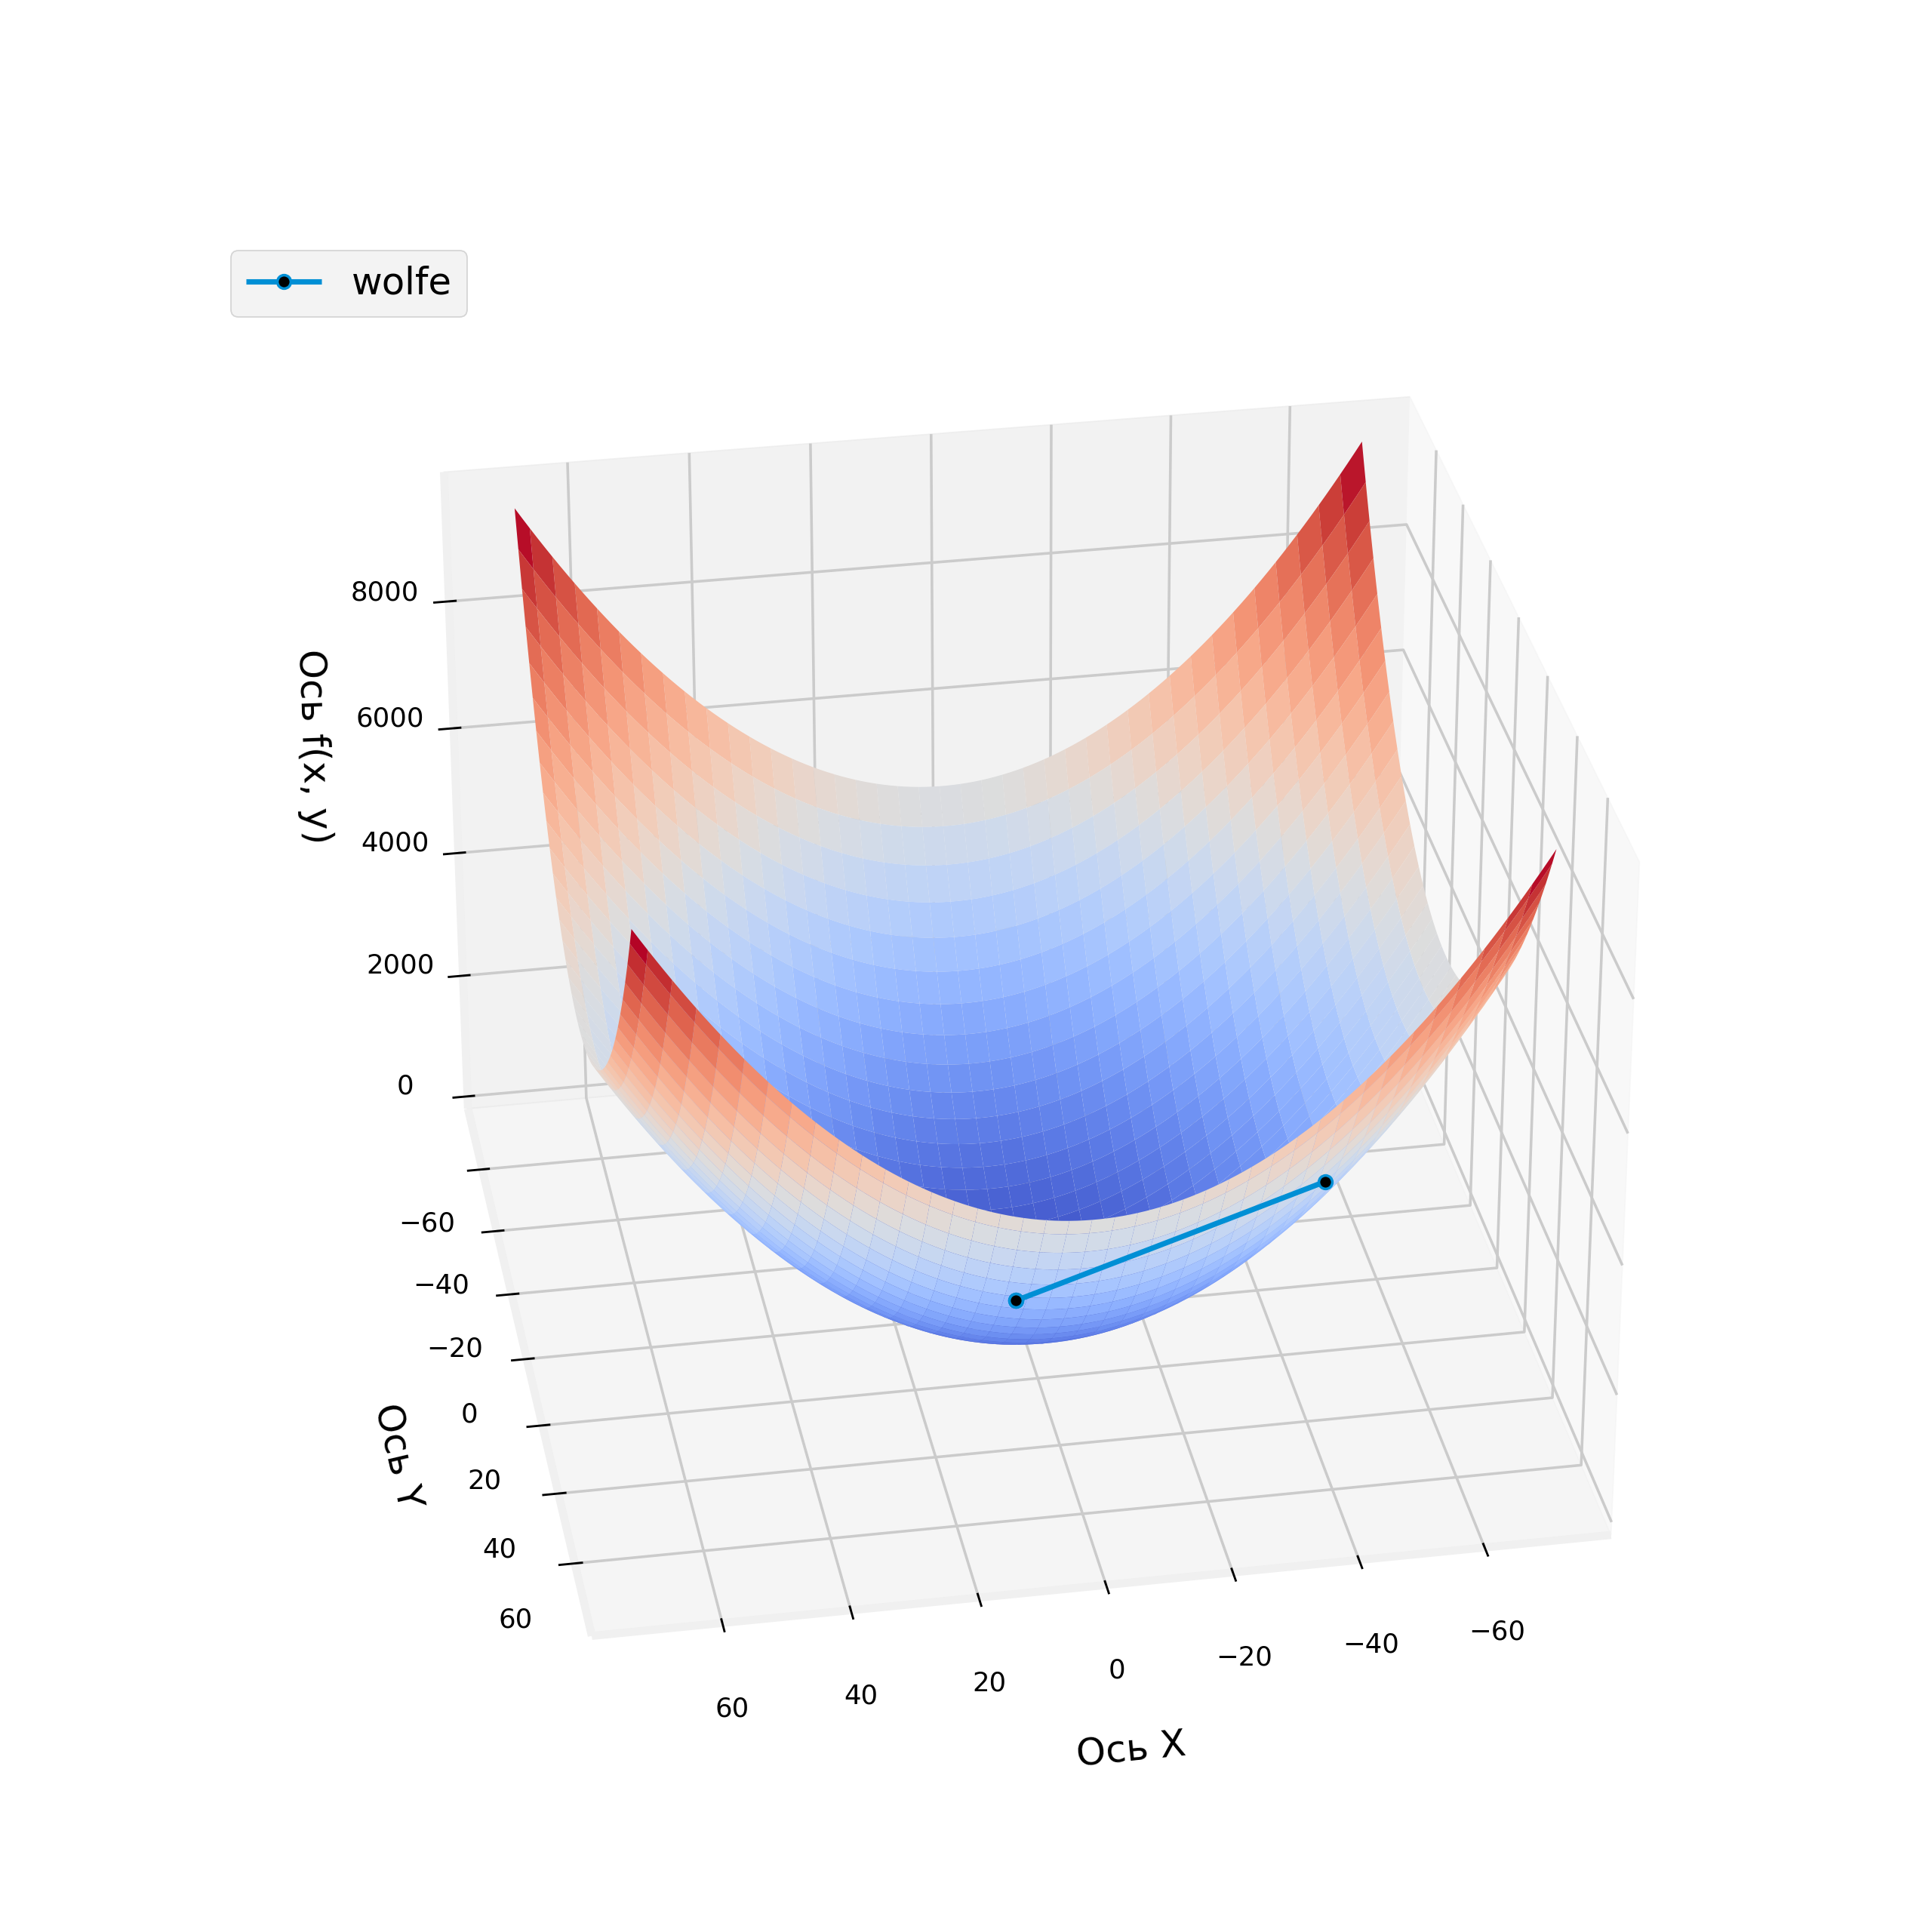
\includegraphics[scale=0.68]{Image/T8_F1.png}
		\caption*{\texttt{T8\_F1}}
	\end{figure}
	Также сразу же предоставим на общее обозрение полученные результаты хода алгоритма.
	\begin{table}[H]
		\centering
		\begin{tabular}{|c|c|c|}
			\textbf{X} & \textbf{Y} & \textbf{F(X, Y)} \\ \hline
			-40 & 50 & 4100 \\
			0.0177669 & -0.0222086 & 0.000808884 \\
			5.70083e-08 & -1.70503e-08 & 3.54066e-15 \\
			-5e-13 & -5e-13 & 5e-25
		\end{tabular}
	\end{table}
	Заметим, что метод нахождения константы с условие Вольфе сильно ускорил работу поиска приближенного минимума, в сравнении с методом дихотомии (понятное дело, обычный метод градиентного спуска не в счет). Почему это так происходит? Опять же засчёт того, что в первом случае мы не могли менять как-либо наш шаг, только если уменьшать его или не изменять его. Если бы мы задали методу дихотомии такую же длину шага, что и первый шаг Вольфе, то получили такие же бы результаты.
\end{document}
